% Dokumentklassen:
% article, report, beamer, book, letter etc.
% https://en.wikibooks.org/wiki/LaTeX/Document_Structure
\documentclass[a4paper]{article}

% Seitenränder Abstand setzen
\usepackage[margin=80pt]{geometry}

% Deutsches Sprachpaket
\usepackage[ngerman]{babel}
% UTF8 Input Encoding
\usepackage[utf8]{inputenc}

% Schriftbild ändern
% https://en.wikibooks.org/wiki/LaTeX/Fonts
\usepackage[scaled]{helvet}
% (Sans) Serifen oder anderes
% \rmdefault: Serifen
% \sfdefault: Sans-Serifen
% \ttdefault: Typewriter
\renewcommand{\familydefault}{\sfdefault}
% Fontencoding (für ä, ö, ü etc.)
\usepackage[T1]{fontenc}

% Gänsefüsschen richtig kompilieren
\usepackage [autostyle]{csquotes}
\MakeOuterQuote{"}

% Hyperlinks farblos
\usepackage[hidelinks]{hyperref}
\hypersetup{colorlinks=false}

% Package für Aufzählungen
\usepackage{enumitem}
% kein Abstand zwischen Aufzählungen
% Sollen doch Abstände vorhanden sein: nach Aufzählung {itemsep=1em}
\setlist{nosep}

% Grafik-Packages, für Figures, Subfigures und PDF als Import
\usepackage{graphicx}
\usepackage{subcaption}
\usepackage{pdfpages}

\title{\textbf{PMRE - Project Management \& \\
		Requirements Engineering}\\
Zusammenfassung}
\date{\today}
\author{Maurin D. Thalmann}

\begin{document}
	
	\pagenumbering{gobble}
	\maketitle
	
\newpage
	\pagenumbering{arabic}
	\tableofcontents
	
\newpage
	
	\section{Project Management - MTW in der Projektabwicklung}
	
		% TODO evtl. Einleitende Gedanken beifügen
	
		\subsection{Projektarbeit \& -Abwicklung}
		
		\begin{description}
			\item[Systemgestaltung] Ein System um- oder neugestalten, um ein erkanntes Problem (unbefriedigenden Zustand) zu lösen
			\item[Problemlösungsprozess (makro)] Problemlösungsvorgehen anwenden, welches durch Projektorganisation und prozessuelles Vorgehen (Phasenplan) strukturiert wird
			\item[Projektmanagement] Projektleitung dirigiert Problemlösungsprozess nach vorgegebener Art und Weise, um Erfolg des Vorhabens sicherzustellen
			\item[Problemlösungszyklus (mikro)] Projektteam wendet im Laufe der Problemlösung Methoden, Techniken, Werkzeuge an, um ein optimales Zielsystem zu gestalten
		\end{description}
	
				\paragraph{Projekt}
				
				Ein Projekt beinhaltet alle Tätigkeiten, um einen IST-Zustand (Problem) in einen Soll-Zustand (Lösung) zu überführen
				
				\paragraph{Projektabwicklung}
				
				Projektabwicklung legt den Fokus auf die Art und Weise der Abwicklung eines Projekts, um ein vereinbartes Projektziel zu erreichen. 
				Meist wird eine vorgegebene Art und Weise des Vorgehens für die konkrete Abwicklung genutzt (Projektmethode a.k.a. Vorgehensmodell oder Vorgehensmethode).
				
				\paragraph{Unterscheidung Projektmanagement vs. Systemgestaltung}
								
				\begin{description}
					\item[Projektmanagement] Fokus auf das Management des Problemlösungsprozesses, die Planung und Disposition der Ressourcen, die Organisation der Informationsflüsse, der Meinungsbildungs- und Entscheidungsprozesse etc.
					\item[Systemgestaltung] auch System Engineering; Fokus auf die Problemlösung im eigentlichen Sinne, die effektive Um- oder Neugestaltung eines Systems
				\end{description}
			
			\subsubsection{Aufgaben des Projektmanagement}
			
			Projektmanagement als Sammelbegriff für alle planenden, überwachenden, koordinierenden und steuernden Tätigkeiten, welche zur erfolgreichen Durchführung der Systemgestaltung notwendig sind.
			Das Vorgehen zur Erreichung der Lösung steht im Vordergrund (nicht das System an sich).
			Projektmanagement lässt sich in folgende Dimensionen gliedern:
			\vspace{1em}
			\begin{description}
				\item[Funktionale Dimension] Alle Aufgaben der Ingangsetzung, Inganghaltung und dem Abschluss eines Projekts
				\item[Institutionale Dimension] dalle Aufgaben, um formale Organisations- und Entscheidungseinheiten zu schaffen, welche im Projekt etabliert werden (Projektteams, Gremien und Rollen)
				\item[Instrumentale Dimension] Alle Aufgaben der Definition, Einführung und Unterhalt von Methoden und Werkzeugen zur zeitlichen, kapazitiven, qualitativen und kostenbezogenen Planung, Überwachung und Steuerung eines Projekts
				\item[Personelle Dimension] Alle personenbezogenen Komponenten in einem Projekt, Wahl von Mitarbeitenden, Zusammenarbeit, Kommunikation, Konfliktbewältigung etc.
				\item[Psychologische Dimension] Alle personenbezogenen Aspekte eines Projekt, bezogen auf Akzeptanz der Ziele, Vorgehensweisen, Verhaltensmuster, Sinnhaftigkeit des Vorhabens durch Mitarbeiter.
			\end{description}
		
			\subsubsection{Aufgaben der Sytemgestaltung}
			
			Bei Systemgestaltung steht die eigentliche Problemlösung / Lösungsfindung im Vordergrund.
			Somit das eigentliche Problem selbst, gedanklicher Lösungsansatz, Abgrenzung zur Umwelt, Anforderungen, die Lösung im engeren inhaltlichen Sinne, Aspekte des Entwurfs, der Architektur des Aufbaus der Lösung, die detaillierte Ausgestaltung etc.
			
\newpage
			
			\paragraph{Gesamtheitliche Sicht auf die Projektabwicklung}
			
			Die beiden Makroprozesse des Projektmanagement und der Systemgestaltung ergeben eine gesamtheitliche Sicht auf die Abwicklung von Projekten:
		
			\begin{figure}[!htb]
				\centering
				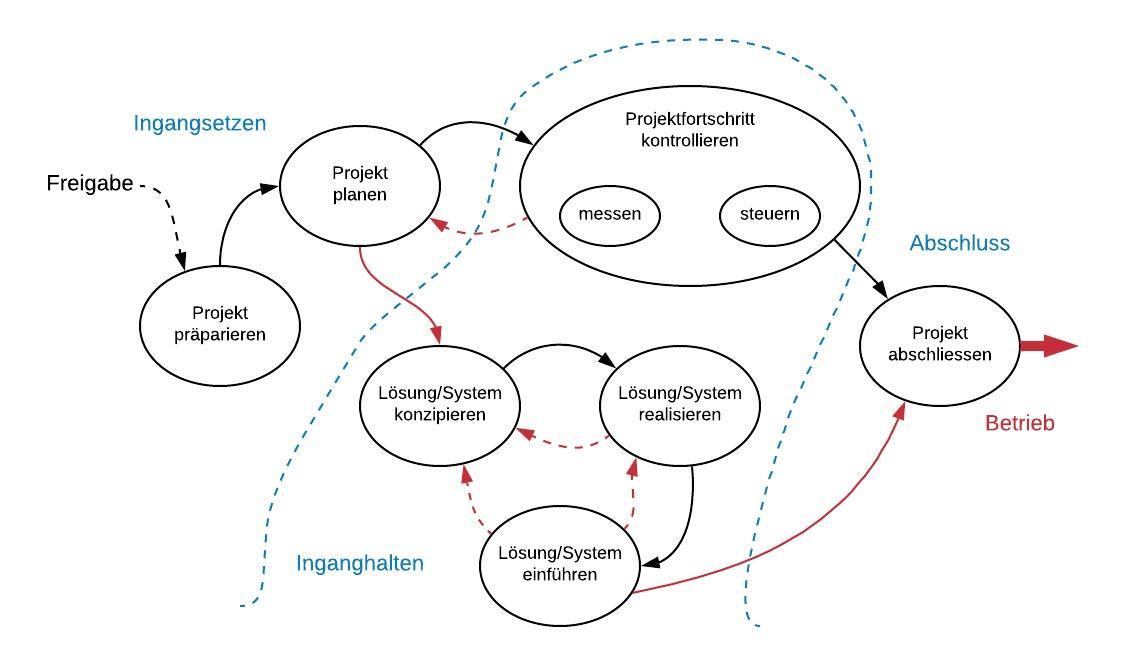
\includegraphics[keepaspectratio, height=8cm]{img/pm/project_view.jpeg}
				\caption{Gesamtheitliche Sicht auf Mikroprozesse der Projektabwicklung}
				\label{fig:pm_projectview}
			\end{figure}
		
			\paragraph{Business Case}
			
			Neuere Denkmodelle beinhalten ebenfalls die Betriebsphase in den Projektüberlegungen.
			Der effektive Erfolg eines Projekts manifestiert sich erst in langjähriger Anwendung des erhaltenen Systems, der Erfolg eines Projekts kann also erst in der Betriebsphase wirklich überprüft werden.
			In einigen Projektmethoden wird der Erstellung und ständiger Überprüfung des Business Case hohes Gewicht zugesprochen.
			Der \textbf{Business Case} ist die unternehmerische Rechtfertigung eines Projekts.
			
			\paragraph{Phasenkonzept \& Meilensteine}
			
			Ein Projekt wird wesentlich in Phasen unterteilt, um die Gesamtaufgabe in sinnvolle, besser überschaubare Teile zu gliedern.\\
			\textit{Projektphase:} zetlicher Abschnitt eines Projektablaufs, sachlich von anderen Abschnitten getrennt.\\
			\textit{Meilenstein:} beschreibt Zustand einer Leistung, eines oder mehrere entscheidende Lieferobjekte, die in definierter Qualität bis zu einem bestimmten Zeitpunkt mit entsprechenden Kosten erstellt werden müssen.\\
			Phasen bilden die Schnittstelle zwischen Projektmanagement und Systemgestaltung.
			Sie erlauben offizielle "Marschhalte" in der Projektabwicklung.
			Meilensteine trennen die einzelnen Schritte der Makroprozesse, können aber auch in einzelnen Projektschritten angewendet werden. 
			
	\subsection{Projektmanagement}
	
		\subsubsection{Projektmethoden}
		
		Eine Projektmethode ist ein auf einem Regelsystem aufbauendes Verfahren zur Erlangung praktischer Ergebnisse.
		Sie beinhaltet somit auch Themen der Aufbauorganisation, von Rechten und Pflichten (AVK - Aufgaben, Verantwortung und Kompetenzen), von normativen Vorgaben, von funktionalen, institutionellen, instrumentellen und personellen Aspekten.
		Sie definiert sich in einem kasualen / prozessualen Modell (bspw. Vorgehensmodell) und zusätlichen Beschreibungen (Rollen, Organisation, Verantwortlichkeiten, Standards etc.)
		Sie können wiederverwendet werden und dienen als Orientierungshilfen für andere Personen mit ähnlichen Problemen / Projekten.
		
\newpage
		
			\paragraph{Herausforderung / Nutzen}
			
			Die Herausforderung ist, für ein bestimmtes Projekt die geeignetste Projektmethode zu eruieren und korrekt anzuwenden.
			Eine korrekte Projektmethode hilft dabei...
			\vspace{1em}
			\begin{itemize}
				\item ... Qualität, Termin- und Kostentreue zu verbessern / einzuhalten
				\item ... Abwicklungseffizienz von Projekten zu verbessern
				\item ... unterstützt Beteiligte in Projekten bei der Führung und Durchführung
				\item ... unterstützt Projektleitung durch Einsatz standartisierter Werkzeuge
				\item ... Kommunikation innerhalb Projektteam / Unternehmen / externer Stakeholder zu verbessern
				\item ... gewonnenes Know-How (best practices) wieder anzuwenden, somit von anderen zu profitieren
				\item ... Projekte untereinander besser zu koordinieren (Priorisierung) und aufeinander abzustimmen (Ressourceneinsatz)
				\item Abhängigkeiten zu Personen \& Firmen zu reduzieren
			\end{itemize}
		
			\paragraph{Typisierung von Projektmethoden}
			
			Da in einem Projekt überlicherweise ein Produkt / System realisiert wird, sollte man die Typisierung aufgrund von Produkteigenschaften vorzunehmen. Es sind bereits folgende Methoden bekannt:
			\vspace{1em}
			\begin{itemize}
				\item Traditionelle Methode - Wasserfall (sequentielle Methoden, plan-driven)
				\item Agile Methode - Scrum (inkrementelle methoden, event-driven)
				\item Hybride Methoden - SoDa (Software Development agile)
			\end{itemize}
	
		\subsubsection{Grundlegende Denkansätze bei Projektmethoden}
			
			\paragraph{Konstruktivistischer (sequenzieller) Ansatz}
			
				\begin{itemize}
					\item Vollständiges Produkt wird in einem Durchlauf zu 100\% Umfang (nach Zielen und Anforderungen) realisiert und am Ende des Entwicklugnszyklus zur Einführung oder zum Kauf freigegeben
					\item Ziel / Zielgrösse wird nach deren Festlegung nicht mehr verändert
					\item Alles zu 100\%: Einführung als Big Bang oder parallel zu altem System
					\item Typischer Ansatz für monolithische Systeme (bspw. Bauwerk (Tunnel), neue SW-Lösung etc.)
				\end{itemize}
		
			\paragraph{Inkrementeller Ansatz}
			
				\begin{itemize}
					\item Eigenständiger Teil des Gesamtprodukts vollständig fertigstellen und freigeben, weitere eigenständige Teile werden parallel / verzögert oder anschliessend fertiggestellt und freigegeben
					\item 1. Teil zu 100\% fertiggestellt, ein 2. Teil ebenfalls zu 100\%, n-ter Teil ebenfalls etc.
					\item Ziel/Ziele (Zielgrösse) werden nach Festlegung nicht mehr verändert
					\item Typischer Ansatz für modulare Systeme wie Standard-SW mit versch. Modulen, welche unabhängig voneinander realisiert \& eingeführt werden können
				\end{itemize}
			
			\paragraph{Evolutionärer Ansatz}
			
				\begin{itemize}
					\item Ganzes Produkt wird initial auf einem tiefen Funktions- / Qualitätslevel fertiggestellt und freigegeben, in weiterer Entwicklungsstufe wird das Produkt funktional / qualitativ weiterentwickelt
					\item Pro Stufe/Release immer grösserer Funktionsumfang
					\item Ziel / Ziele (Zielgrösse) kann nach jedem Release verändert werden, muss aber nicht, und dies immer aufbauend auf dem bestehenden Release-Stand
					\item Typischer Ansatz bei unklaren Aufgabenstellungen
				\end{itemize}
			
			\paragraph{Iterativ / Iterationen}
			
			\textit{Inkrementell} und \textit{evolutionär} sind iterative Ansätze, da sie die Phasen mehrmals durchlaufen.
			
			\paragraph{Auswahl an Vorgehensmodellen}
			
			PmBoK - Project Management Book of Knowledge, 
			Hermes - der Eidgenosse, 
			Prince 2, 
			ISO 21500:2012, 
			DIN 69901, 
			Wasserfall, 
			diverse V-Modell(e), 
			Kanban, 
			Scrum, 
			DevOps, 
			SAFe, 
			(fast) Prototyping, 
			eXtreme Programming (XP), 
			Rational Unified Process (RUP), 
			Lean Project Management, 
			6-Sigma, 
			ICB (IPMA Competence Baselines), 
			firmenspezifische Projektmanagement-Systeme (PMS), 
			ITIL - IT Infrastructure Library (mehr als eine PM), 
			CMMI - Capatiblity Maturity Model Integration, 
			System Engineering (SE, mehr als eine PM)
			
\newpage
	
	\subsection{Systemgestaltung}
	
	Die Wissenschaft der Gestaltung von Systemen nennt sich System Engineering (SE).
	Dazu gibt es ein ganzes Buch, welches aber nicht zum Stoff gehört.
	Folgendes Denkmodell soll jedoch veranschaulichen, welche Kompetenzbereiche dem System Engineering angehören:
	
	\begin{figure}[!htb]
		\centering
		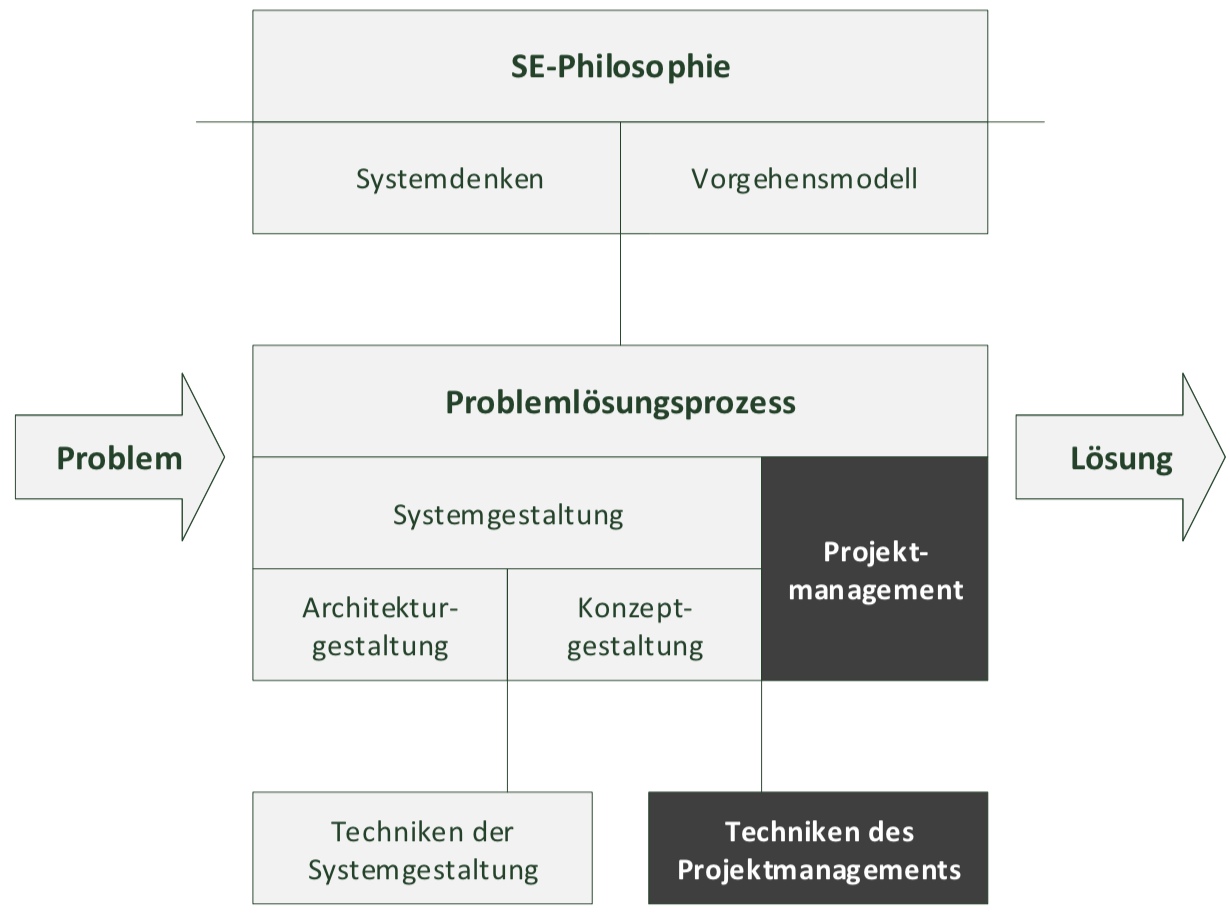
\includegraphics[height=7cm]{img/pm/denkmodell.png}
		\caption{Denkmodell zum System Engineering}
		\label{fig:pm_se_denkmodell}
	\end{figure}
\noindent
	\textit{Projektmanagement} in diesem Modell ist Teil des übergeordneten \textit{Problemlösungsprozesses}; 
	anderer Teil ist der gestalterische Aspekt der Projektarbeit (\textit{Systemgestaltung}).
	Dies ist unterteilt in die Disziplinen \textit{Architekturgestaltung} und \textit{Konzeptgestaltung}.
	Architekturgestaltung enthält das grundlegende Lösungsprinzip, Konzeptgestaltung die konkrete \& umsetzungsorientierte Ausarbeitung der Lösung.
	Folgt dem Denkansatz "Vom Groben zum Detail".\\
	Randbedingungen sind eine immer komplexere Welt (vernetzter und dynamischer), gekoppelt mit ungenügenden Informationen darüber.
	
		\subsubsection{Systemdenken}
		
		Systemdenken wird definiert als eine Denkweise, die es ermöglicht, komplexe Erscheinungen  (= Systeme) besser verstehen und gestalten zu können. 
	
		\subsubsection{Systemmerkmale und -Struktur}
	
			\paragraph{Elemente \& Beziehungen}
			\vspace{1em}
				\begin{itemize}
					\item \textbf{Systeme} bestehen aus \textbf{Elementen (Komponenten)}
					\item Elemente haben Eigenschaften und Funktionen
						\begin{itemize}
							\item \textbf{Eigenschaften} können Attribute sein (Farbe, Material, Zustand etc.)
							\item \textbf{Funktionen} geben Zweck eines Elements in konkretem Kontext wieder
						\end{itemize}
					\item Elemente können als Systeme betrachtet werden, die man wiederum in Elemente gliedern kann
					\item Elemente sind untereinander durch \textbf{Beziehungen} verbunden.
					Beziehungen können gerichtet sein (wirkungsorientiert). 
					Beziehungen können als Informationsflüsse, Materialflüsse, Lagebeziehungen etc. verstanden werden.
					\item Elemente können dynamisch sein (zu unterschiedlichen Zeitpunkten eine unterschiedliche Ausprägung haben).
					Solche dynamischen Systeme werden als komplex betrachtet.
				\end{itemize}
		
			\paragraph{Ordnung}
			
			Elemente \& Beziehungen stellen ein Gefüge / eine Einheit dar und weisen dadurch eine Ordnung auf.
			Die Ordnung wird als eine Struktur welche \textit{hierarchisch}, \textit{sternförmig} oder \textit{any-to-many (Netzstruktur)} sein kann.
			
		\subsubsection{Darstellungsarten}
		
		Zur Darstellung von Systemen bieten sich folgende Arten an:
		\vspace{1em}
		\begin{itemize}
			\item Graphen / Knoten-Kanten-Diagramme, Elemente werden als Knoten (Kreise/Rechtecke), Beziehungen als Kanten (Pfeile, gerichtete/ungerichtete Beziehungen) dargestellt
			\item Graphen / CLD gemäss Sterman, einensich zur Darstellung der Dynamik von Systemen
			\item Matrizen, Elemente als Spalten/Zeilen, Beziehungen in jeweiligen Knotenpunkten markieren
		\end{itemize}
	
		\subsubsection{Denkansätze und Betrachtungsweisen}
		
		\begin{description}
			\item[Blackbox] Innere Struktur eines Systems interessiert in der Betrachtung nicht, nur Inputs und Outputs.
			Hilfreich, um die Komplexität zu reduzieren.
			\item[Whitebox] Innere Struktur (Zusammenhang Inputs/Outputs) ist für die Betrachtung von hoher Relevanz.
			Wenn das System bspw. weiter unterteilt oder simuliert werden soll.
			\item[Greybox] Zwischenform der Detailierung, System ist grob und teilweise strukturiert.
			\item[Aspekte] Systeme unter verschiedenen Gesichtspunkten analysieren.
			Je nach Nutzer interessiert jeden ein anderer Aspekt des gesamten Systems.
		\end{description}
	
		\subsubsection{Systemtypen}
		
			\paragraph{Einfaches System}
			
			Einfach zu verstehen und beschreiben.
			Typisiert sich, indem es nur wenige Elemente aufweist, welche durch wenige, nicht-dynamische Beziehungen verbunden sind.
			Einfache Systeme können in ihrer Gesamtheit explizit beschrieben werden.
			
			\paragraph{Kompliziertes System (massiv vernetzt)}
			
			Wenn Anzahl und Vielfalt von Komponenten \& Beziehungen zunehmen, nennt man es ein massiv vernetztes kompliziertes System.
			Beziehungen sind jedoch immer noch nicht-dynamisch.
			Durch Systemgrösse wird es jedoch sehr schwierig, ein solches System explizit zu beschreiben.\\
			$\rightarrow$ Technische Systeme
			
			\paragraph{Kompliziertes System (dynamisch)}
			
			Beziehungen zwischen Elementen verändern sich über die Zeit, sowohl hinsichtlich der Art der Interaktion, Stärke und Struktur.
			Solche Systeme sind aufgrund dynamischer Beziehungen schwierig quantitativ zu beschreiben bzw. ihr Verhalten vorherzusagen.\\
			$\rightarrow$ Sozio-technische Systeme\\
			$\rightarrow$ Technische Systeme
			
			\paragraph{Komplexes System}
			
			Hohe Vielfalt und hohe Dynamik in den Beziehungen zeichnen ein komplexes System aus.
			Sind sehr schwer, wenn überhaupt, zu beschreiben.
			
		\subsubsection{Anwendung des Systemdenkens im Projektmanagement}
		
		SEUSAG-Analyse als sytemtheoretischer Ansatz zur Bestimmung des Projektgegenstandes\\ 
		(resp. zum Umgang mit Komplexität)
		\vspace{1em}
		\begin{description}
			\item[S] Systemgrenzen bilden
			\item[E] Einflussgrössen ermitteln
			\item[U] Unter- und Teilsysteme abgrenzen
			\item[S] Schnittstellen definieren
			\item[A] Analyse der Unter- und Teilsysteme
			\item[G] Gemeinsamkeiten ermitteln
		\end{description}
	
			\paragraph{Agilität von Systemen}
			
			Man muss mit dem Gedanken spielen können dass es eine Anforderung sein kann, ein agiles Lieferobjekt zu erstellen und nicht nur agil vorzugehen.
			Dies muss unterschieden werden können und wird im dazugehörigen Dokument vom ILIAS genauer beschrieben. \textit{(agile SYSTEMS Engingeering versus AGILA SYSTEMS Engineering)}

\newpage

		\subsubsection{Dynamik von Systemen}
		
			\paragraph{Policy Resistance}
			
			Sozio-technische Systeme verhalten sich selten wie vorhergesagt oder erwünscht.
			Dieses Phänomen der "Policy Resistance" wird darin begründet, dass Menschen die Feedbacks ihrer Handlungen nicht versehen und ein rein lineares Denken in Abfolgen praktizieren\\
			$\rightarrow$ Event-oriented View\\
			\\
			Unsere Aktionen verändern jedoch den Zustand eines Systems, andere Teilnehmer des Systems reagieren um das Gleichgewicht wiederherzustellen.
			Aktionen haben immer Nebeneffekte zur Folge, welche erkannt werden müssen.\\
			$\rightarrow$ Feedback-oriented View
			
			\paragraph{Feedback Loops}
			
			Die höchste Komplexität resultiert aus den Interaktionen zwischen Komponenten, nicht von den Komponenten selbst.
			Es werden zwei Arten von Feedback Loops unterschieden:
			\begin{itemize}
				\item Positive Loops (self-reinforcing)
				\item Negative Loops (self-correctiong, balancing)
			\end{itemize}		
			Ein System besteht, unabhängig der Komplexität, aus einer Struktur von positiven und negativen Feedbacks.
			Die Systemdynamik stammt aus den Interaktionen zwischen diesen Feedback Loops.
			Feedbacklogik wird in Causal Loop Diagrams (CLD) dargestellt.
	
			\begin{figure}[!htb]
				\centering
				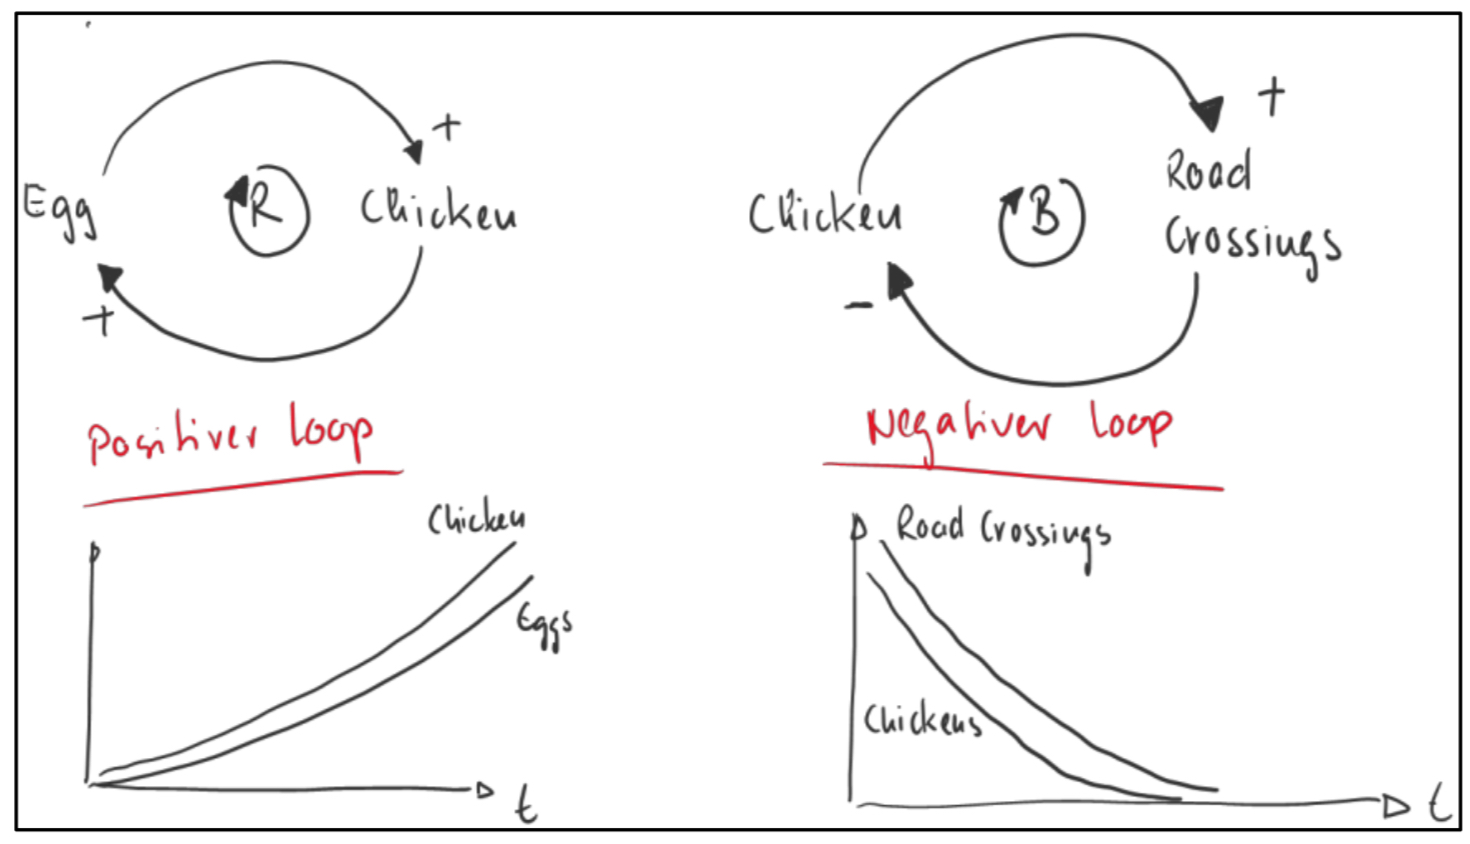
\includegraphics[height=5cm]{img/pm/feedback_loop.jpeg}
				\caption{Causal Loop Diagram als Beispiel}
				\label{fig:pm_feedback_loops}
			\end{figure}
		
			\begin{description}
				\item[+]Effekt steht positiv in Beziehung zur Ursache\\ 
							(mehr/weniger vom einen hat mehr/weniger vom anderen zur Folge) 
				\item[-] Effekt steht negativ in Beziehung zur Ursache\\
							(mehr/weniger von einen hat mehr/weniger vom anderen zur Folge)
			\end{description}
		
\newpage
		
		\subsubsection{SE-Vorgehensmodell}
	
		Im Software Engineering definiertes Vorgehensmodell, bestehend aus 4 Pfeilern / Komponenten, die in Kombination angewendet werden.
	
			\paragraph{Top-Down - Vom Groben ins Detail}
			
				\begin{itemize}
					\item \textit{Grundidee}:\\
					Von der Blackbox zur Whitebox, Details verhindern oft den Blick auf das Ganze.
					\item Das Betrachtungsfeld weiter fassen und schrittweise einengen.
					Betrifft die Untersuchung des Problemfelds, der Ausgangssituation und den Entwurf von Lösungen.
					\item Bei Untersuchung der Ausgangssituation (Problemfeld) nicht mit detaillierten Erhebungen beginnen, bevor das Problemfeld grob strukturiert, in seine Umwelt eingebettet / gegen sie eingegrenzt ist und Schnittstellen definiert sind (oft auch nur Arbeitshypothese)
					\item Bei Lösungsgestaltung erst generelle Ziele \& Lösungsrahmen festlegen.
					Detaillierungs- und Konkretisierungsgrad im Verlauf der Projektarbeit schrittweise vertiegen.
					Konzepte auf höheren Ebenen als Orientierungshilfen für detaillierte Ausgestaltung der Lösung.
				\end{itemize}
			
			\paragraph{Variantenbildung - Denken in Varianten}
			
				\begin{itemize}
					\item \textit{Grundidee}:\\
					Vielfalt von Lösungsmöglichkeiten Rechnung tragen
					\item Unverzichtbarer Bestandteil guter Planung.
					Methodische Grundhaltung, muss nicht zu nennenswertem zusätzlichem Arbeitsaufwand führen.
					\item Nichtbeachtung: grosses Risiko, dass andere Lösungsansätze erst später im Projektverlauf eingebracht werden.
					Konsequenzen wären Abwürgen der Diskussion, Planungsstopp und Rückkehr auf eine höhere Ebene.
				\end{itemize}
			
			\paragraph{Projektphasen - Makrologik}
			
				\begin{itemize}
					\item \textit{Grundidee}:\\
					Gliedern eines Projekts nach zeitlich-logischen Gesichtspunkten zur Kontrolle von Komplexität
					\item Nach zeitlichen Gesichtspunkten gegliedertes Raster, hilft den Werdegang eines Lösung in überschaubare Teiletappen zu gliedern.
					\item Stufenweiser Planungs-, Entscheidungs-, Realisierungsprozess mit vordefinierten Marschhalten / Korrekturpunkten, reduziert Komplexität der Projektabwicklung und schafft Lernchance für Planenden, Durchführenden \& Auftraggeber.
					\item Konzept kann im Sinne einer Makrologik als managementorientierte Komponente gesehen werden.
					Fordert zwischen Entwicklert \& Arbeitgeber/Management an vordefinierten Stellen eine Kontaktaufnahme, Willensbildung und Entscheidung.
				\end{itemize}
			
			\paragraph{Problemlösungszyklus - Mikrologik}
	
				\begin{itemize}
					\item \textit{Grundidee}:\\
					Systematisches Vorgehen bei Auftreten jeder Art von Problemen in jeder Phase des Projekts
					\item Als eine Art Mikrologik ein Leitfaden zur Behandlung von Problemen oder Aufgabestellungen, in jeder Phase eines Projekts anwendbar.
				\end{itemize}
	
\newpage
		
		\subsubsection{Problemlösungszyklus - PLZ}
	
		\begin{itemize}
			\item \textbf{Problem}: Differenz zwischen "Ist-" und "Soll-Zustand"
			\item Versuchs-Irrtum-Methode (try and error): natürliche Art und Weise, Mensch kann jedoch den Try \& Error Prozess vorwegnehmen, bevor er eine Entscheidung treffen muss.
			Er besitzt die Fähigkeit, Folgen seines Handelns abzuschätzen.
			Dies erlaubt ihm systematische Vorgehen zur Problemlösung.
		\end{itemize}
	
		\paragraph{Design Thinking}
		
			Möglichkeit zur systematischen Vorgehensweise zum Problemlösen.
			
			\begin{figure}[!htb]
				\centering
				\begin{subfigure}{.5\textwidth}
					\centering
					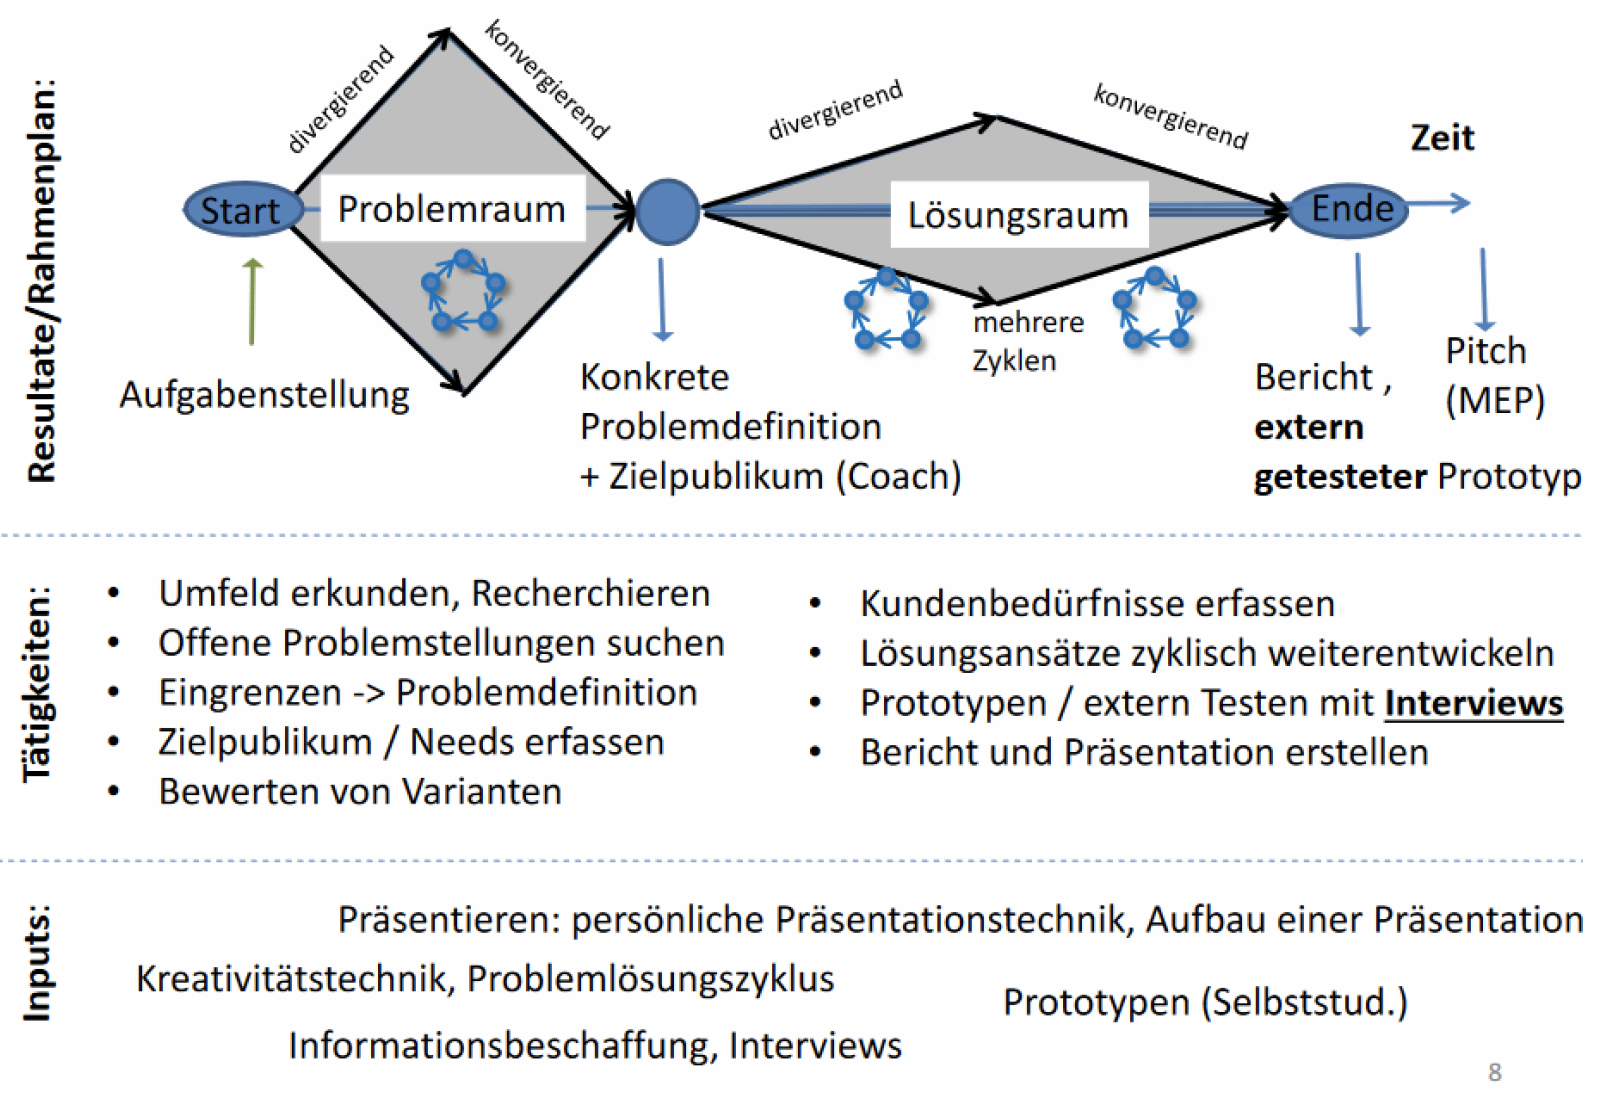
\includegraphics[height=5.5cm]{img/pm/design_thinking.png}
					\caption{Design-Thinking-Zyklus}
					\label{fig:pm_designthinking}
				\end{subfigure}
				\begin{subfigure}{.4\textwidth}
					\centering
					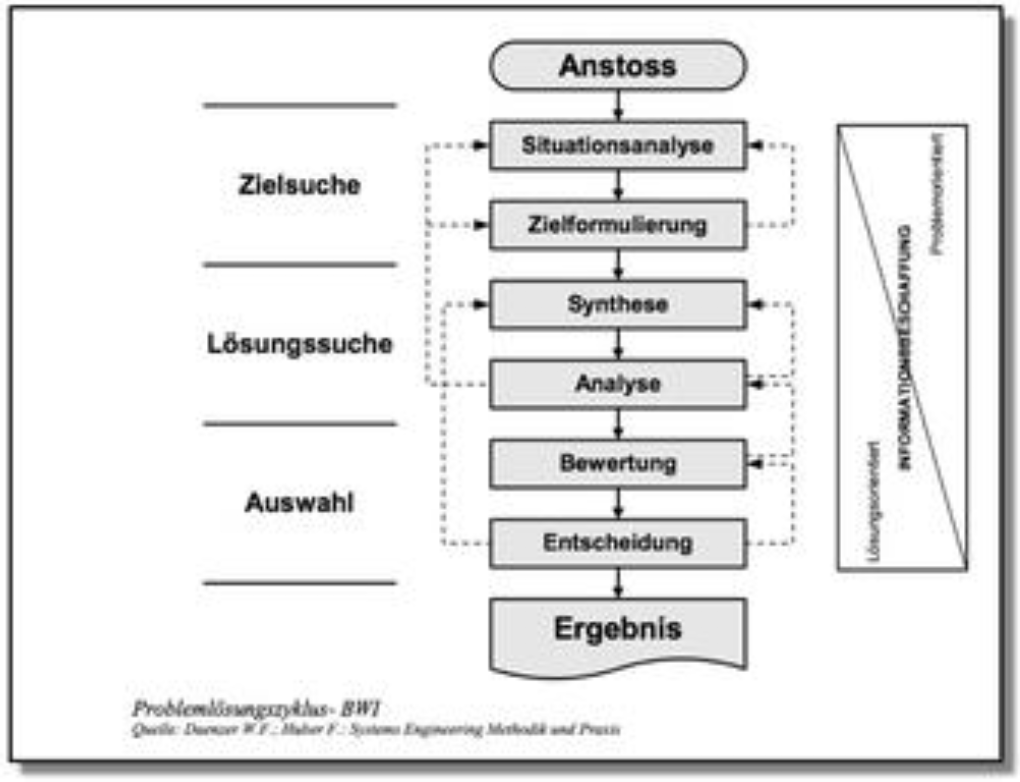
\includegraphics[height=4cm]{img/pm/plz.png}
					\caption{Problemlösungszyklus}
					\label{fig:pm_plz}
				\end{subfigure}
			\end{figure}
			\noindent		
			Der \textbf{Anstoss} setzt den PLZ in Gange.
			Er startet entweder das ganze Projekt oder befindet sich innerhalb einer Phase oder eines Arbeitspaketes als Auslöser des PLZ.
				
		\paragraph{Problemlösungszyklus - Zielsuche}
		
			\begin{itemize}
				\item Teilschritte der Zielsuche sind die \textit{Situationsanalyse} und \textit{Zielformulierung}
				\item Zweck der \textbf{Situationsanalyse}:
					\begin{itemize}
						\item Erarbeitung grundlegendes Verständnis bzgl. des Problems, dessen Erscheinungsformen sowie Ursachen und deren Zusammenhänge
						\item Strukturierung \& Abgrenzung des Problems bzw. Untersuchuntsfelds
						\item Definition des Eingriffs- und Gestaltungsbereichs für Lösungssuche
						\item Schaffung der notwendigen Informationsbasis für nachfolgende Arbeitsschritte
					\end{itemize}
				\item Zweck der \textbf{Zielformulierung}:
					\begin{itemize}
						\item Alle Ziele, die zur Lösung eines Problems erreicht werden, müssen möglichst\\
						\textit{vollständig, präzise und verständlich, realistisch} und \textit{lösungsneutral} definiert werden
						\item Unterscheiden zwischen Muss-, Soll- und Wunschzielen\\
								$\rightarrow$ Diese Unterscheidung setzt Prioritäten der Ziele in der Projektabwicklung
						\item Zielvorstellung(-en) können bereits durch \textit{Anstoss} vorgegeben sein
						\item Durch diese beiden Teilschritte sollen Randbedingungen einer Problemlösung definiert werden, es darf keineswegs ein bestimmter Lösungsweg vorgegebern werden\\ ($\rightarrow$ Lösungsneutralität der Ziele)
					\end{itemize}
				\item Methoden/Techniken/Werkzeuge:
					\begin{itemize}
						\item \textbf{Informationsbeschaffung:} Befragung, Beobachtung, Checklisten, Fragebogen, Interview, Panelbefragung, Prognosen, Stichproben etc.
						\item \textbf{Informationsaufbereitung:} ABC-Analyse, Ablaufdiagramm, Analysetechniken, Benchmarks, Korrelationsanalyse, Math-Statistik, Regressionsanalyse, Schwachstellenanalyse etc.
						\item \textbf{Informationsdarstellung:} Darstellungstechniken, Mind Maps, Input-Output-Methode etc.
						\item \textbf{Zielformulierung:} Operationalisierung, Target Costing, Use Case etc.
					\end{itemize}
			\end{itemize}
	
\newpage
		
		\paragraph{Problemlösungszyklus - Zielsuche}
		
			\begin{itemize}
				\item Teilschritte der Lösungssuche sind \textbf{Synthese} und \textbf{Analyse} von Lösungen
				\item Zweck der \textbf{Synthese}:
					\begin{itemize}
						\item Sammlung \& Ausarbeitung von Lösungsalternativen.
						\item Kreativer, aufbauend-konstruktiver Schritt, baut auf Resultaten der Situationsanalyse auf (Situationskenntnis, Problemverständnis, Zielformulierungen, Anforderungskatalog)
					\end{itemize}
				\item Zweck der \textbf{Analyse}:
					\begin{itemize}
						\item Machbarkeit einer Lösungsalternative verifizieren\\ 
						(ohne zu werten oder mit anderen Alternativen zu vergleichen, erfolgt in \textit{Auswahl})
						\item Kritischer, analytisch-destruktiver Schritt
						\item Erfüllt eine Lösungsalternative die Ansprüche nicht, kann sie verworfen werden oder muss überarbeitet werden
					\end{itemize}
				\item Methoden/Techniken/Werkzeuge:
					\begin{itemize}
						\item \textbf{Synthese - Kreativität:} Analogiemethode, Bionik, Brainstorming, Just in Time, Kärtchentechnik, Kreativitätstechniken, Morphologie etc.
						\item \textbf{Synthese - Optimierung:} Operations Research, Dynamische Optimierung, Entscheidungsbaum, Lineare Optimierung, Spieltheorie, Warteschlangenmodelle, Use Case etc.
						\item \textbf{Analyse:} FMEA, Fehlerbaumanalyse, Gefährdungsanalyse, Reverse Engineering, Risk Management, Schwachstellenanalyse, Total Quality Control, Wert-Analyse etc.
					\end{itemize}
			\end{itemize}
		
		\paragraph{Problemlösungszyklus - Zielsuche}
		
			\begin{itemize}
				\item Teilschritte der Auswahl sind \textbf{Bewertung} und \textbf{Entscheid}
				\item Zweck der \textbf{Bewertung}:
					\begin{itemize}
						\item Taugliche Lösungsvarianten gegenüberstellen (jene, welche alle Muss-Ziele erfüllen)
						\item Formale Bewertung wird angezeigt, wenn keine Variante als Beste identifiziert werden kann
						\item 3 Bedingungen müssen erfüllt werden:
							\begin{itemize}
								\item Min. 2 echte Lösungsalternativen müssen existieren
								\item Bewertungskriterien (bezogen auf Zielformulierungen) müssen definiert sein
								\item Bewerter müssen Alternativen hinsichtlich Bewertungskriterien beurteilen können
							\end{itemize}
					\end{itemize}
				\item Zweck des \textbf{Entscheids/Auswahl}:
					\begin{itemize}
						\item Basierend auf Bewertungsergebnissen die weiter zu bearbeitende Variante bestimmen
					\end{itemize}
				\item Methoden/Techniken/Werkzeuge:
					\begin{itemize}
						\item \textbf{Bewertung \& Entscheidung:}
						Analytic-Hierarchie-Process, Bewertungstechniken, Entscheidungstheorie/-baumverfahren, Kosten-Nutzen-Analyse, Kriterienplan, Nutzwerkanalyse, Wirtschaftlichkeitsrechnung, Punktbewertung etc.
					\end{itemize}
			\end{itemize}
			\vspace{1em}
			Es kann sein dass PLZ keine zufriedenstellende Variante hervorbringt.
			Oder dass sich das Projekt mit verfügbaren Mitteln nicht realisieren lässt.
			Es sind Schlussfolgerungen möglich:\\
			\begin{itemize}
				\item Projektabbruch
				\item Sistierung der Zusammenarbeit mit Systementwicklern
				\item Zielreduktion
				\item Zurück auf höhere Systemebene, mit anderen Wegen zum Ziel kommen
				\item Problem neu umschreiben / definieren
			\end{itemize}
			
\newpage
		
		\begin{figure}[!htb]
			\centering
			\begin{subfigure}{.45\textwidth}
				\centering
				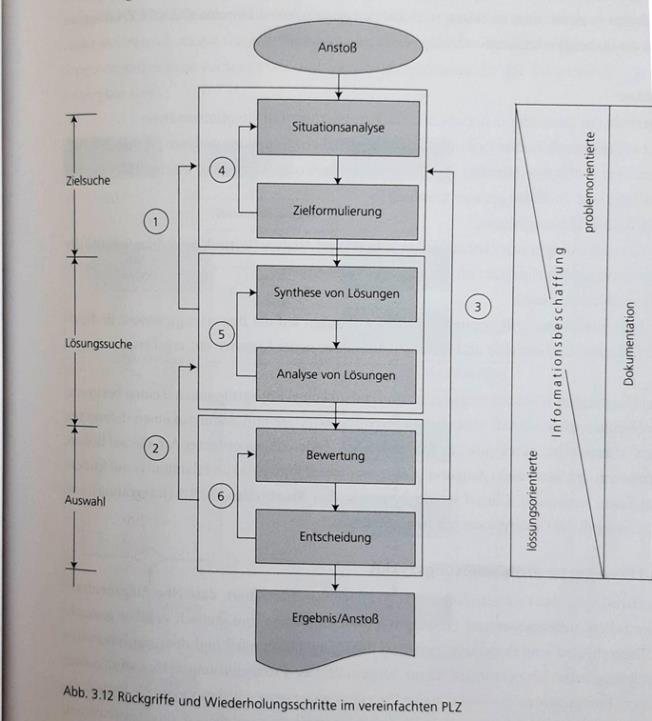
\includegraphics[height=8cm]{img/pm/plz_teile.jpg}
				\caption{Aufteilung des PLZ in Grob-/Feinzyklen}
				\label{fig:plz_teile}
			\end{subfigure}
			\begin{subfigure}{.45\textwidth}
				\centering
				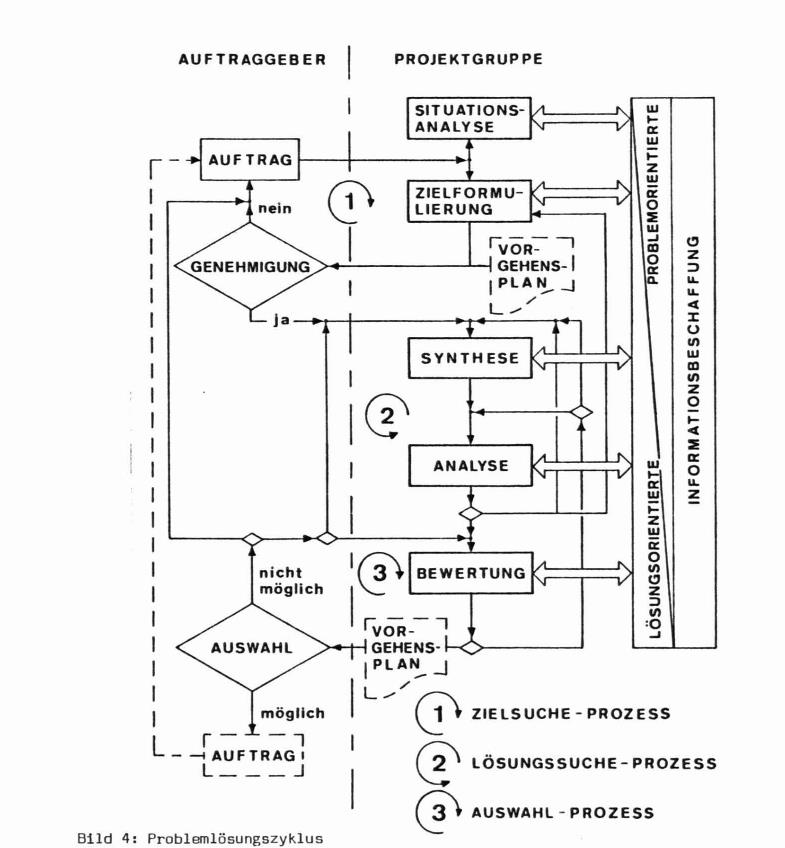
\includegraphics[height=8cm]{img/pm/plz_ext.jpg}
				\caption{Erweiterter PLZ}
				\label{fig:plz_ext}
			\end{subfigure}
		\end{figure}
		
		\paragraph{Erweiterter PLZ}
		
		Im Erweiterten PLZ werden die Schritte bezogen auf Rollen Auftraggeber und Projektgruppe unterschieden.
		Unter Projektgruppe ist auch der Projektmanager miteinbezogen, welcher den PLZ begleitet und führt.
	
	\subsection{Erfolgsmuster in der Projektarbeit}
	
		\paragraph{Erfolg / Misserfolg?}
		
		\begin{itemize}
			\item \textbf{Wer} entscheidet darüber?\\
					Auftraggeber, Stakeholder, Endbenutzer des neuen Systems?
			\item \textbf{Wann} wird darüber entschieden?\\
					Nach Projektende, nach Teil der Nutzungsphase?
			\item Zusätzliche Themen: Standish Chaos Report, PMI (Dokumente dazu im ILIAS)
		\end{itemize}
	
	
\newpage
	
	\section{Project Management - Projekt in Gang setzen}
	
		\subsection{Projekt präparieren}
		
			\paragraph{Projektorganisation}
			
			Massgebende Entscheidungsgremien initialisieren:
				\begin{itemize}
					\item Reine Projektorganisation / Linien-PO
					\item Stab-Linien-Projektorganisation / Projektkoordination
					\item Matrix-Projektorganisation
					\item Mischformen
				\end{itemize}
			
			\paragraph{(Erste) Ziele setzen}
			
			Ziele sollen Lösungssuche steuern und eine Lösung nicht nachträglich rechtfertigen.
			Erarbeitung der Zielsetzungen ist Tätigkeit des Projektmanagements.
			Zielsuche ist die erste Phase des PLZ, Zielformulierung der 2. Schritt.
			
		\subsection{Zielbegriff}
		
			\paragraph{Definitionen}
			
				\begin{itemize}
					\item Ziel: angestrebter Zustand / erwünschte Wirkung
					\item Zukünftige Ergebnisse, die durch Massnahmen / Lösungen erreicht werden sollen
					\item Ziele sollen bekannt sein, bevor Ermittlung der Anforderungen begonnen wird
					\item Jede Anforderung muss sich auf ein Ziel zurückführen lassen
					\item Unterscheiden zwischen:
						\begin{itemize}
							\item \textbf{Abwicklungsziele}\\
							Unterteilt in Leistungs-, Qualitäts-, Zeit/Termin- und Kostenziele
							\item \textbf{Systemziele}\\
							Fokussieren auf Akzeptanz \& Wirtschaftlichkeit des zu erstellenden Systems. Hierarchisch unterteilt in Global-, Gruppen- und Detailziele
						\end{itemize}
					\item Ziele sollen folgenden Prinzipien folgen:
						\begin{itemize}
							\item Wertorientierung
							\item Lösungsneutralität (keine mögliche Lösung favorisieren / vorgeben)
							\item Operationalität (Ziel-Mittel-Denken)
							\item Vollständigkeit der Zielinhalte
							\item Berücksichtigung der wichtigen Informationsquellen \& Interessenslagen
							\item Feststellbarkeit der Zielerfüllung
							\item Prioritätensetzung
								\begin{description}
									\item[Muss-Ziele] müssen zwingend eingehalten werden
									\item[Soll-Ziele] hohe Bedeutung, wenn möglich einhalten
									\item[Wunschziele] tiefe Verbindlichkeit, "nice to have"
								\end{description}
							\item Widerspruchsfreiheit, Zielkonflikte vermeiden / eliminieren
							\item Überblickbarkeit \& Bewältigbarkeit des Zielkatalogs
						\end{itemize}
				\end{itemize}
			
			\paragraph{Zielformen}
			
			\begin{description}
				\item[Abwicklungsziele] Bezug auf Projektmanagement, geben vor was bei Meilensteinen konkret vorliegen muss (Lieferobjekte, Meilensteinplan)
				\item[Vorgehensziele] Bezug auf Projektmanagement, geben vor wie das Projekt abgewickelt wird, bspw. systematisches Stakeholder-Management durchführen
				\item[Systemziele] Bezug auf Systemgestaltung, Teil des Problemlösungsprozess.
				Sagen aus was mit zu gestaltender Lösung erreicht / vermieden werden soll (Zustand).
			\end{description}
	
		\subsection{Anforderungsbegriff}
		
			\begin{itemize}
				\item Anforderung: eine Aussage über eine Eigenschaft oder Leistung eines Produkts, Prozess oder der am Prozess beteiligten Personen
				\item Unterscheidung:
					\begin{description}
						\item[Ziel] Zustand
						\item[Anforderung] Eigenschaft (Verhalten, Fähigkeit, Funktion)
					\end{description}
			\end{itemize}
		
\newpage
		
		\subsection{Ziel-Mittel-Denken}
		
		\begin{itemize}
			\item Kann ein Ziel ("WAS") zu einem Mittel ("WIE") werden?
			\item Ziel-Mittel-Denken: Instrument zur Entwicklung und Operationalisierung von Zielen
			\item Nutzt zur Visualisierung eine Ziel-Mittel-Hierarchie
			\item Prinzip der Lösungsneutralität muss jederzeit sichergestellt sein!
		\end{itemize}
	
		\begin{figure}[!htb]
			\centering
			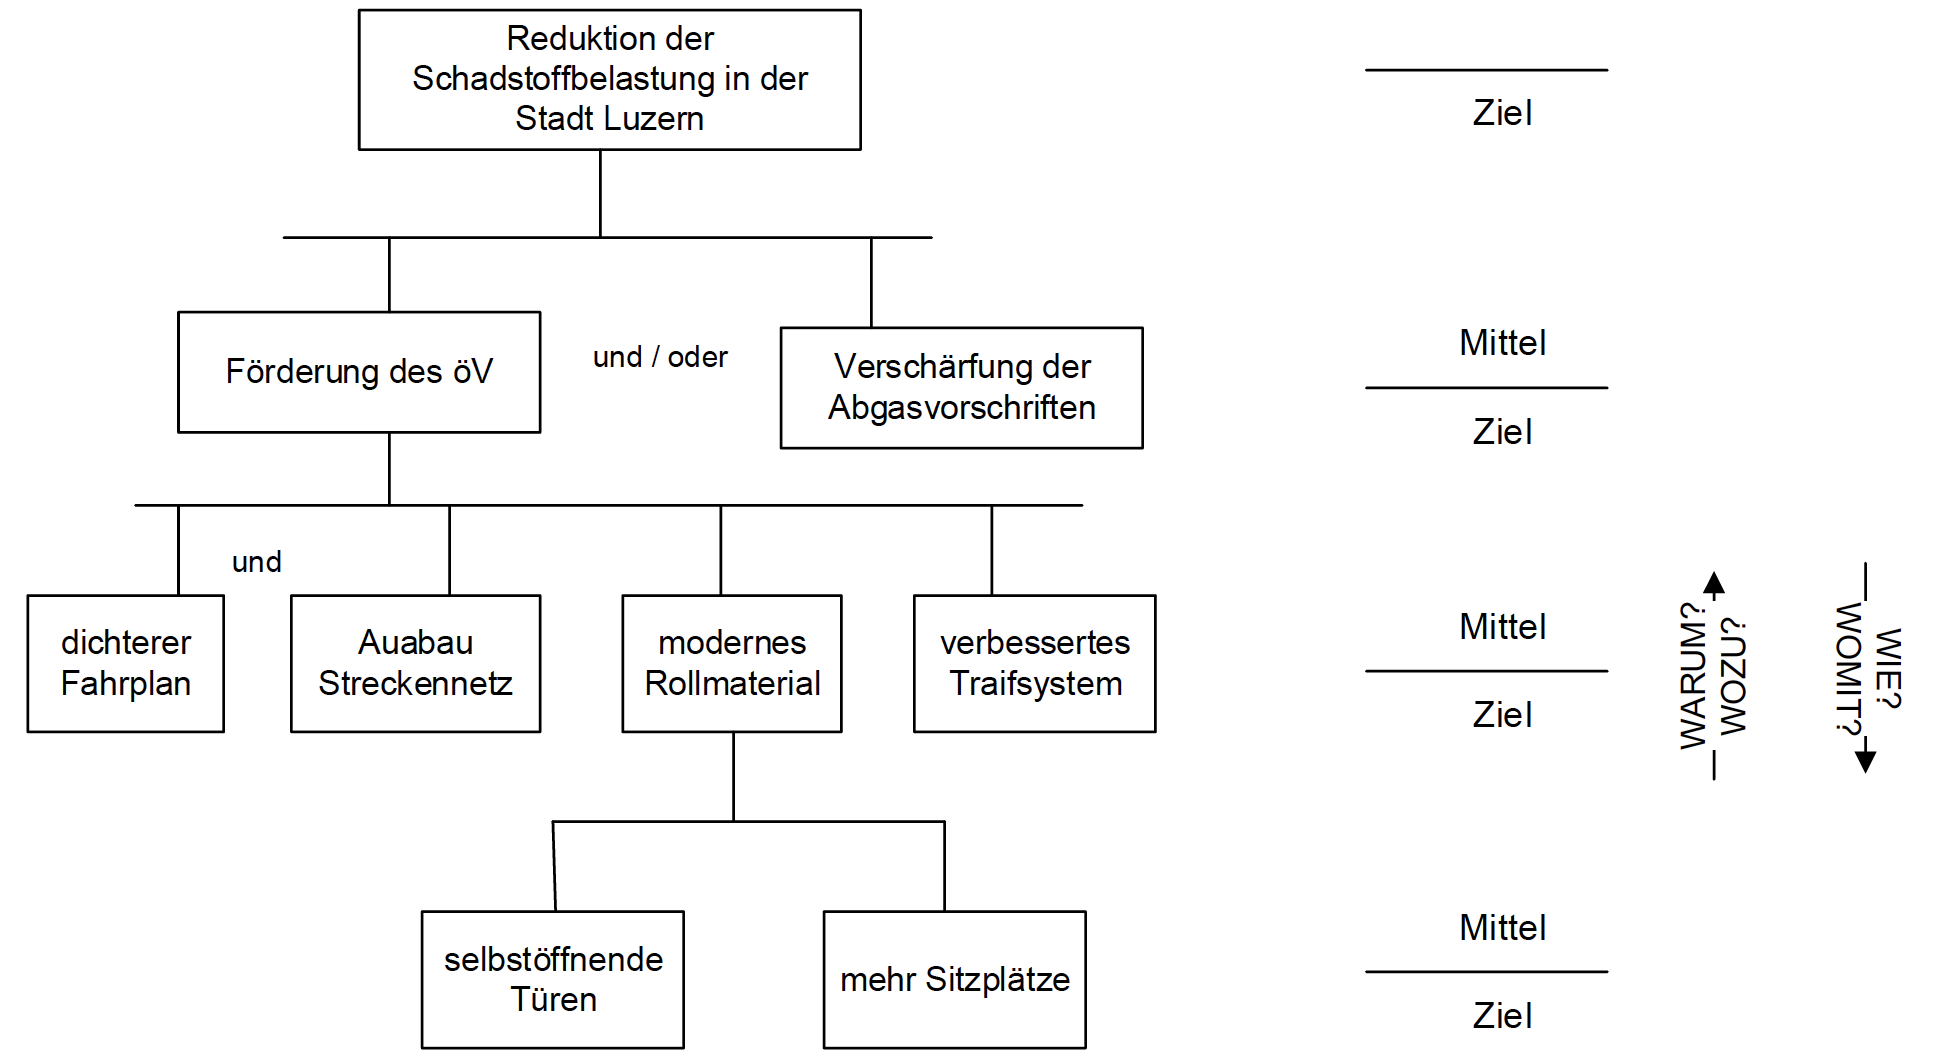
\includegraphics[height=6cm]{img/pm/zmd.png}
			\caption{Ziel-Mittel-Denken}
			\label{fig:pm_zmd}
		\end{figure}
	
		\paragraph{S.M.A.R.T. Objectives}
		
			\begin{itemize}
				\item Ziele sollten möglichst SMART sein:
					\begin{description}
						\item[S] Spezifisch\\
						Grenzen des Zielbereichs werden vorgegeben, für konkrete Organisation o.ä.
						\item[M] Messbar\\
						Qualitäten / Quantitäten der Zielerreichung bestimmbar, Indikatoren ableitbar
						\item[A] Angemessen\\
						Das "richtige" Ziel? Besteht Bedarf für geplante Massnahme?
						\item[R] Realistisch\\
						Aussichten, Ziel zu erreichen, unter Rahmenbedingungen ausreichend hoch
						\item[T] Terminiert\\
						Zeitlicher Rahmen wird vorgegeben
					\end{description}
				\item Ziele müssen nicht auf jeder Stufe s.m.a.r.t. formuliert sein
				\item Zur Messbarkeit der Zielerreichung: Prinzip der Feststellbarkeit der Zielerfüllung (Kap. 2.2)\\ $\rightarrow$ setzt s.m.a.r.t.e Formulierung voraus
			\end{itemize}
		
\newpage
		
		\subsection{Zielrelationen (-Matrix)}
		
		Ziele können in unterschiedlicher Beziehung zueinander stehen.
		Ziele sollen dem Prinzip der Widerspruchsfreiheit georchen.
		Dazu werden alle aufeglisteten Ziele auf ihre Relationen überprüft.
		
			\begin{itemize}
				\item sich gegenseitig unterstützen (\textbf{unterstützend})
					\begin{itemize}
						\item Erreichung von Ziel A unterstützt Erreichung von Ziel B und umgekehrt
						\item \textbf{angenehm}
					\end{itemize}
				\item unabhängig voneinander sein (\textbf{indifferent})
					\begin{itemize}
						\item Erreichung Ziel A ist unabhängig von Erreichung Ziel B und umgekehrt
						\item \textbf{problemlos}
					\end{itemize}
				\item \textbf{gegenläufig} sein (Gegenläufigkeit / Zielkonkurrenz)
					\begin{itemize}
						\item Ziel A \& B behindern sich: Je besser A erreicht wird, umso schlechter kann B realisiert werden und umgekehrt
						\item \textbf{Kompromisse müssen gefunden werden}
					\end{itemize}
				\item Im Konflikt zueinander stehen (\textbf{widersprüchlich}, Zielkonflikt)
					\begin{itemize}
						\item Ziel A und B logisch oder situationsbedingt im Konflikt, \\
						können nicht gleichzeitig nebeneinander existieren
						\item \textbf{Konflikt muss aufgelöst werden}
							\begin{itemize}
								\item Prioritäten setzen (Muss, Soll, Wunsch)
								\item Auflösung des Konflikts durch Innovation
								\item Einführung von Mindest- und Höchstwerten
								\item Streichen eines Konfliktverursachers							
							\end{itemize}
					\end{itemize}
			\end{itemize}
		
		\subsection{Zielgewichtung}
		
		Nicht alle Ziele sind gleich wichtig, sie müssen gewichtet werden.
		
			\subsubsection{Paarvergleich}
			
			Methode zur Bestimmung und Berechnung der Präferenzen / Gewichtung von Zielen oder Kriterien untereinander.
			Funktionsweise: Jedes Ziel wird mit jedem anderen 1:1 verglichen und ein "Sieger" bestimmt.
			
			\begin{quote}
				Mögliche Kombinationen im Paarvergleich: $K=\frac{n(n-1)}{2}$
			\end{quote}
		
			\subsubsection{Präferenzmatrix}
			
			Instrument zum Paarvergleich und der Berechnung der Gewichtung.
			Jede Zielkombination wird mit dem Sieger (a ist wichtiger als b) benennt.
			2 Möglichkeiten zur Berechnung des Gewichts:
			
			\begin{quote}
				$Gewicht[\%] = \frac{Anzahl Nennungen \cdot 100}{Total Nennungen}$\\
				\\
				$Gewicht[\%] = \frac{umgedrehterRang \cdot 100}{Summe Aller Raenge}$\\
				\\
				\textit{(2. Variante hat den Vorteil, dass Ziele ohne Nennung ein Gewicht erhalten \\
				und nicht 0\% Gewichtung haben)}
			\end{quote}
		
			\begin{figure}[!htb]
				\centering
				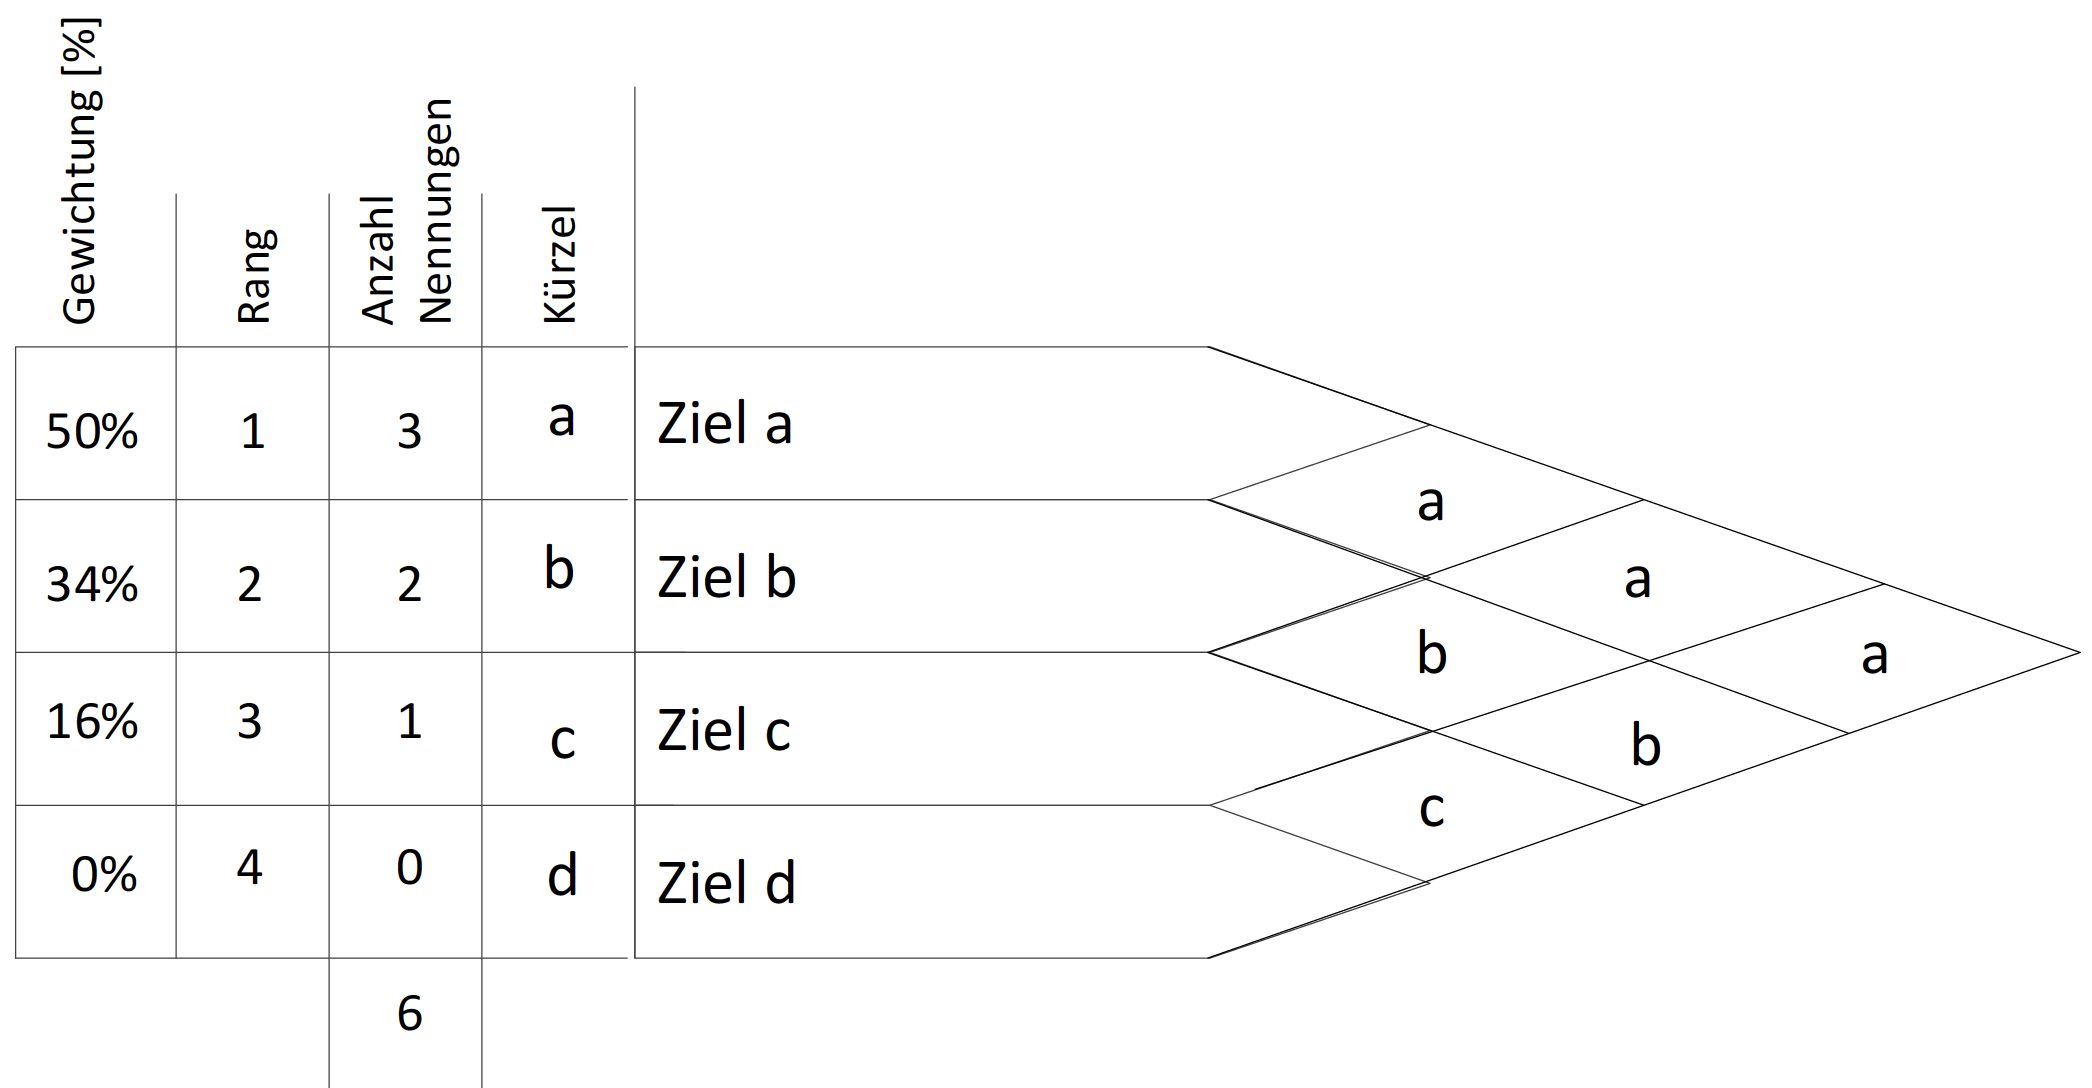
\includegraphics[height=3.7cm]{img/pm/prefmatrix.png}
				\caption{Beispiel Gewichtung in Präferenzmatrix}
				\label{fig:prefmatrix}
			\end{figure}
	
\newpage
	
		\subsubsection{Analytical Hierarchy Process (AHP)}
		
		Alternative Methode zur Berechnung der Zielgewichte.
		Man kann hiermit bestimmen, um wieviel ein Ziel wichtiger ist als ein anderes.
		Zur Berechnung wird jedoch Vektorgeometrie benötigt, was wir dann gar nicht angeschaut haben.
		
		\subsubsection{Lieferobjekte aus "Projekt präparieren"}
		
		Aus diesem ersten Schritt resultiert ein Projektantrag, welches als Vertrag für die Aufnahme der aufwändigen Planungsaktivitäten dient.
		
		\begin{quote}
			Ziel $\rightarrow$ Projektantrag liegt im Status "approved" vor\\
			Lieferobjekt $\rightarrow$ Projektantrag, freigegeben
		\end{quote}
	
	\subsection{Projekt planen (Planungsprozess)}
	
	Im Planungsprozess werden Pläne (= dokumentarische Lieferobjekte) entwickelt.
	Sie beinhalten Planung, sind gleichzeitig aber auch immer die erste Analyse der Aufgabenstellung.
	Der Problemlösungszyklus PLZ wird ein erstes Mal durchlaufen.
	Er ist in 9 Schritte aufgeteilt:
	
	\begin{itemize}
		\item \textbf{Meilensteinplanung} $\rightarrow$ Abwicklungszielplan (Meilensteine)
		\item \textbf{Projektstrukturplanung} $\rightarrow$ Projektstrukturplan (Arbeitspakete \& deren Strukturierung)
		\item \textbf{Ablaufplanung} $\rightarrow$ Ablaufplan (Abhängigkeiten, Projektdauer, Pufferzeiten)
		\item \textbf{Ressourcenplanung} $\rightarrow$ Ressourcenplan (Durchlaufzeit (Aufwand) der Arbeitspakete)
		\item \textbf{Organisationsplanung} $\rightarrow$ Organisationsplan (Mitarbeitende zugeteilt auf Arbeitspakete)
		\item \textbf{Kostenplanung} $\rightarrow$ Projektkostenplan (Dokumentierte Kosten \& Finanzierung)
		\item \textbf{Terminplanung} $\rightarrow$ Terminplan (konkrete Termin- und Einsatzplanung)
		\item \textbf{Budgetplanung} $\rightarrow$ Projektbudgetplan (kalendarische Finanzierung)
		\item \textbf{Informationsplanung} $\rightarrow$ Informations-/Dokumentationsplan (Kommunikations-/Infokonzept)
	\end{itemize}

		\subsubsection{Meilenstein- / Phasenplanung}
		
		\begin{description}
			\item[Input] Zielsetzungen an das Projekt (aus Projektantrag)
			\item[Ziel] Bündelung der Ziele \& Umsetzung in definierte Zwischenresultate (Meilensteine)\\
			\textit{Kriterien Meilenstein}: Zeit, Qualität, Lieferobjekt, Aufwand/Kosten
			\item[Output] Definierte Meilensteine
			\item[Lieferobjekt] Abwicklungszielplan
		\end{description}
	
			\paragraph{Phasenplan}
			
			Phasenplan in Anlehnung an gewählte Projektmethode erstellen.
			Es gibt mehrere Möglichkeiten, wie bspw. nur zwei Phasen oder Phasen mit Benennung (Initiieren - Konzipieren - Realisieren - Einführen).
			Man muss nicht zwingend weiter unterteilen, wenn dies nicht nötig ist.
			
			\paragraph{Meilensteinplan}
			
				\begin{quote}
					\textit{Meilenstein beschreibt einen Zustand einer Leistung (ein oder mehrere Lieferobjekte), die bis zu einem bestimmten Zeitpunkt in der definierten Qualität zu den entsprechenden Kosten erstellt werden müssen.}
				\end{quote}
				\noindent
				Meilensteine normalerweise zwischen den Phasen des Phasenplans definieren.
				Es können auch innerhalb von Phasen Meilensteine vorgesehen werden, wenn dies der Absicherung von Risiken oder Qualität sinnvoll erscheint.
				Bei einem Meilenstein wird das Projekt "eingefroren".
				Projekt wird je nach Lieferobjekt in die nächste Phase freigegeben oder Korrekturen an Lieferobjekten werden vorgenommen.
				Meilenstein kann eine "Exit"-Möglichkeit sein, um das Projekt zu stoppen.
		
	
\newpage
		
		\subsubsection{Projektstrukturplanung (PSP)}
		
		\begin{description}
			\item[Input] Meilensteinplan
			\item[Ziel] Gliederung des gesamten Projekts in plan- und kontrollierbare Arbeitspakete
			\item[Output] Definierte Arbeitspakete \& deren Strukturierung
			\item[Lieferobjekt] Projektstrukturplan (PSP)
		\end{description}
	
			\paragraph{Arbeitspaket}
			
				\begin{quote}
					\textit{Ein Arbeitspaket ist eine in sich geschlossene Aufgabenstellung innerhalb eines Projekts.
					Kann bis zu einem festgelegten Zeitpunkt mit definiertem Ergebnis und Aufwand vollbracht werden.}
				\end{quote}
			
			\begin{itemize}
				\item Arbeitspaket ist die tiefste Gliederungsebene des PSP, somit auch die kleinste Planungseinheit
				\item Sie werden einem Projektmitarbeiter oder Projektteam zugeteilt
				\item Faustregeln für den Umfang eines Arbeitspakets:
					\begin{itemize}
						\item Zeit- und Kostenanteil pro AP: 2-5\% des Gesamtprojekts
						\item Dauer in Abhängigkeit des Berichtsintervalls: Faktor 1.5\\
						(bspw. bei Berichtsintervall von 4 Wochen ist Dauer des AP max. 6 Wochen)					
					\end{itemize}
				\item Arbeitspaket soll auch ein "messbares" deliverable beinhalten (analog Meilenstein), da zwischen APs Abhängigkeiten bestehen
				\item Nachläufer (nachfolgendes AP) kann nur gestartet werden, wenn Vorläufer (vorhergehendes AP) korrekt abgeschlossen wurde
				\item Hierarchische Struktur:
					\begin{itemize}
						\item Programm $\rightarrow$ 2-n Projekte $\rightarrow$ 2-n Teilprojekte $\rightarrow$ 2-n Aktivitäten (mündl. Delegation an MA)
					\end{itemize}
			\end{itemize}
		
			\paragraph{PSP - Objekt- oder vorgehensorientiert}
			
				\begin{itemize}
					\item \textbf{Work-Breakdown-Structure (WBS)}\\
					Vorgehensorientierter PSP strukturiert die APs entlang der Phasen, in ihrer logischen zeitlichen Folge.
					Kann als wiederverwertbarer Standardrahmen für die Abwicklung von Projekten in einem Unternehmen genutzt werden.
					\item \textbf{Product-Breakdown-Structure (PBS)}\\
					Objektorientierter PSP (Produktstrukturplan) definiert APs entlang des zu erstellenden Produktes/Systems.
					Einmaliges Werk, kann meistens nicht wiederverwendet werden.
				\end{itemize}
			
			\paragraph{PSP - Wertorientiert}
			
			Wertorientierter PSP macht Sinn, falls der "Wert" eines APs auf den Wert des gesamten Projekts appliziert werden soll.
			Kann sinnvoll sein, wenn bspw. ein AP aus Kostengründen weggelassen werden soll oder nicht.
			
			\paragraph{Formale Regeln im PSP}
			
			AP ist die kleinste Planungseinheit.
			Für Schätzung von Aufwänden in weitere Aktivitäten unterteilbar, muss aber immer wieder zu einem AP zusammengefügt werden.
			\begin{itemize}
				\item AP / Aktivität besteht aus Substantiv + Verb: \textit{Pflichtenheft erstellen}
				\item Meilenstein als Zustand (Ereignis) zu formulieren: \textit{Pflichtenheft erstellt}
			\end{itemize}
			
			\paragraph{Arbeitspaketliste}
			
			Resultat dieses Planungsschritts ist eine Arbeitspaketliste, in welcher alle einzelnen Arbeitspakete erfasst werden.
			
\newpage
		
		\subsubsection{Ablaufplanung}
		
		\begin{description}
			\item[Input] Projektstrukturplan (PSP)
			\item[Ziel] Eruierung von sachlogischen Abhängigkeiten zw. APs \& Durchlaufzeiten von APs
			\item[Output] sachlogische Abhängigkeiten, Projektdauer, Pufferzeiten
			\item[Lieferobjekt] Ablaufplan
		\end{description}
		\vspace{1em}
		Ermittelt für im PSP identifizierte APs die sachlogischen Abhängigkeiten.
		Dazu werden Vorläufer / Nachläufer jedes APs bestimmt.
		Genaue kalendarische Termine sind noch irrelevant, jedoch wird pro AP erste Durchlaufzeit/Dauer geschätzt (aus Erfahrungswerten oder ersten Vorstellungen des PL/Auftraggebers)
		
			\paragraph{Arbeitspaketliste - erweitert}
			
			Für diesen Planungsschritt wird die AP-Liste um den Block \textit{"Vorgänge"} und evtl. auch schon um \textit{"Einsatzmittel"} erweitert. Diese beinhalten jeweils folgende Spalten:
			
			\begin{itemize}
				\item \textbf{Vorgänge}
					\begin{itemize}
						\item Vorgangsdauer (Schätzung der Dauer)
						\item Direkter Vorläufer
						\item Direkter Nachläufer
					\end{itemize}
				\item \textbf{Einsatzmittelbedarf}
					\begin{itemize}
						\item Personal
						\item Sachmittel
						\item Finanzmittel
					\end{itemize}
			\end{itemize}
			
			\paragraph{Schätzung der Dauer von APs}
			
			Dauer, Aufwand und Personaleinsatz noch unbekannt, APs können mit einer fixen Dauer versehen werden.
			Er werden erste Schätzungen der Dauer von APs gemacht für einen ersten Anhaltspunkt der Durchlaufzeit des Projekts.
			Dauer wird so ermittelt, dass ein gewünschter Endtermin des Projekts zustande kommt (ohne Berücksichtigung der effektiven Aufwände \& Ressourcen).
			Kann unter \textit{Vorgangsdauer} in der AP-Liste eingetragen werden.
			
			\paragraph{Sachlogische Abhängigkeit}
			
			Setzt ein Verständnis der Problemstellung voraus.
			Abhängigkeiten werden über die Spalten \textit{Direkter Vorläuger} \& \textit{Direkter Nachläufer} dargestellt.
			Eine grafische Darstellung als Balkendiagramm ist möglich.
			
			\paragraph{Netzplanverfahren}
			
			Ermöglichen Simulationen ("was passiert wenn...") und ein klares Bild der Pufferzeiten wird errechenbar.
			Es existieren mehrere Arten von Netzplanverfahren.
			
			\begin{figure}[!htb]
				\centering
				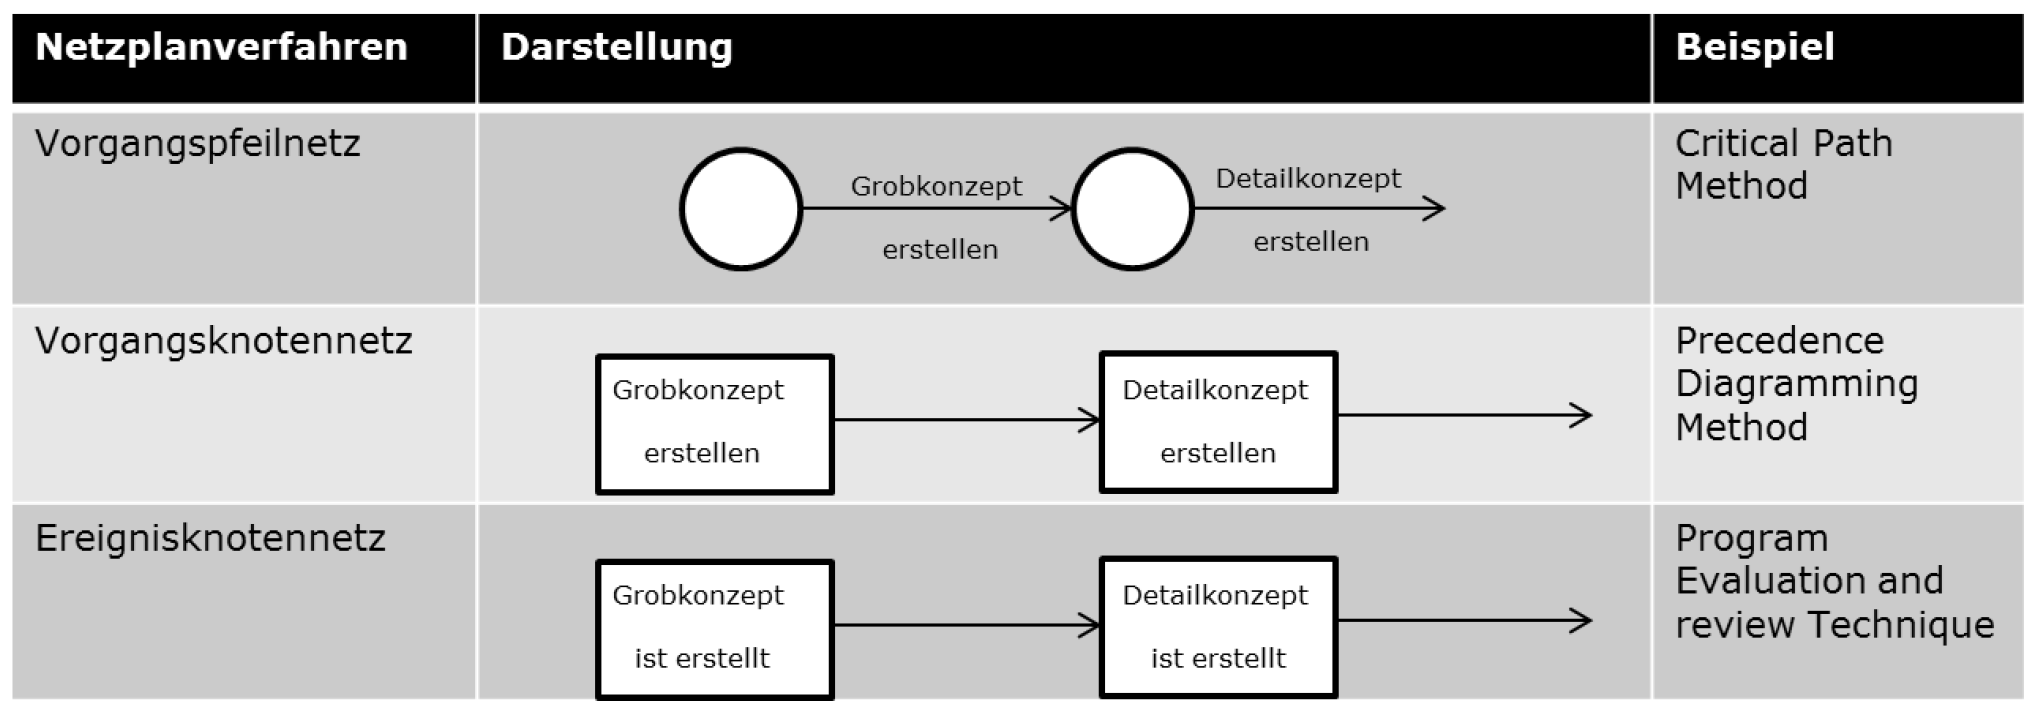
\includegraphics[height=3cm]{img/pm/netzplanverfahren.png}
				\caption{Übersicht der verschiedenen Netzplanverfahren}
				\label{fig:pm_netzplanverfahren}
			\end{figure}
		
			\paragraph{Vorgangpfeil-Netzplan (VPN) - Critical Path Methode (CPM)}
			
			\begin{itemize}
				\item Ziel ist im Netzplan zu erkennen, welche Aktivitäten mit und welche ohne Zeitreserve (kritischer Pfad) durchführbar sind (und somit Ausführungsdauer für das Projekt direkt beeinflussen)
				\item CPM als Planmethode: Darstellungmittel für Teminplanung \& Algorithmus für die Berechnung des kritischen Pfades sowie der Projekt-Gesamtdauer
				\item Netzplan in CPM-Darstellung mit Knoten und Kanten
				\item Ermittlung der Puffer: Aus den unterschiedlichen Zeitpunkten berechnen
			\end{itemize}
		
\newpage
		
			\paragraph{Darstellungsregeln}
			
			\begin{itemize}
				\item \textbf{Knoten}: Darstellungselement für ein Ereignis (Zustand) innerhalb eines Projekts
				\item \textbf{Pfeile/Kanten}: Darstellungselement für einen Vorgang (Tätigkeit, AP) in einem Projekt\\
				(Ein Vorgang entspricht einem AP)
			\end{itemize}
		
			\begin{figure}[!htb]
				\centering
				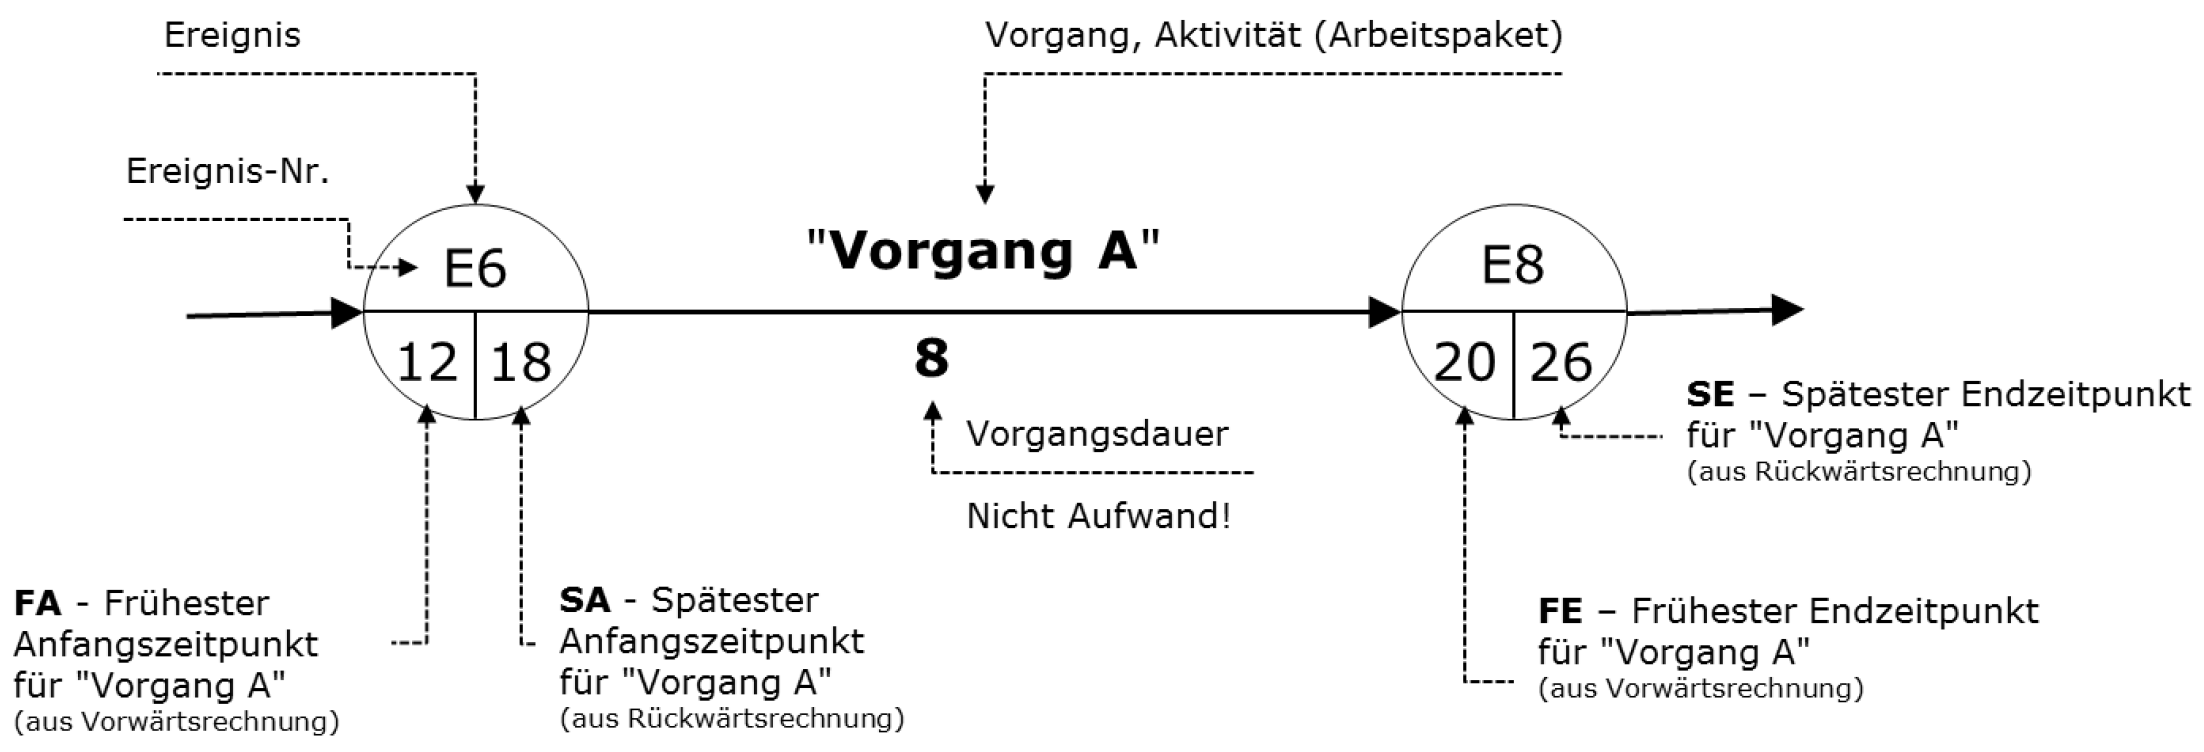
\includegraphics[height=4cm]{img/pm/vpn_notation.png}
				\caption{VPN-Notation von Knoten \& Kanten}
			\end{figure}
		
			\paragraph{Regeln zur Erstellung eines Netzplans nach CPM}
			
			\begin{description}
				\item[Regel 1] Ein Vorgang kann erst beginnen, wenn alle Vorgänger abgeschlossen sind.
						Es fällt das Anfangsereignis mit dem Endereignis des vorhergehenden Vorgans zusammen\\ (Ausnahme erster Vorgang)
						
				\item[Regel 2] Müssen mehrere Vorgänge beendet sein, bevor ein Nachfolger beginnen kann, so enden sie alle im Anfangsbereich des Nachfolgers.
				
				\item[Regel 3] Können mehrere Nachfolger beginnen, nachdem ein Vorgänger beendet ist, so beginnen sie alle im Endereignis des Vorgängers.
				
				\item[Regel 4] Haben zwei oder mehr Vorgänge gemeinsame Anfangs- und Endereignisse, so ist ihre eindeutige Kennzeichnung durch Einfügen von \textbf{Scheinvorgängen} (fiktiver Vorgang mit der Dauer 0) sicherzustellen
				
				\item[Regel 5] Beginnen und enden in einem Ereignis mehrere Vorgänge, die nicht alle voneinander abhängen, muss die Eindeutigkeit ebenfalls durch \textit{Scheinvorgänge} erreicht werden (bspw. Zusammenführung an Meilensteinen)
				
				\item[Regel 6]  In einer Folge von Vorgängen können beliebig viele \textit{Scheinvorgänge} eingefügt werden $\rightarrow$ logische Verknüpfung und bessere Übersicht, so wenig wie möglich einsetzen
				
				\item[Regel 7] Kann ein Vorgang beginnen, bevor der Vorgänger vollständig abgeschlossen ist, muss der Vorgänger unterteilt werden
				
				\item[Regel 8] Jeder Vorgang darf nur einmal ablaufen, es dürfen keine Schleifen auftreten
			\end{description}
			
			\paragraph{Beispiel eines Netzplans nach CPM}
			
			\begin{figure}[!htb]
				\centering
				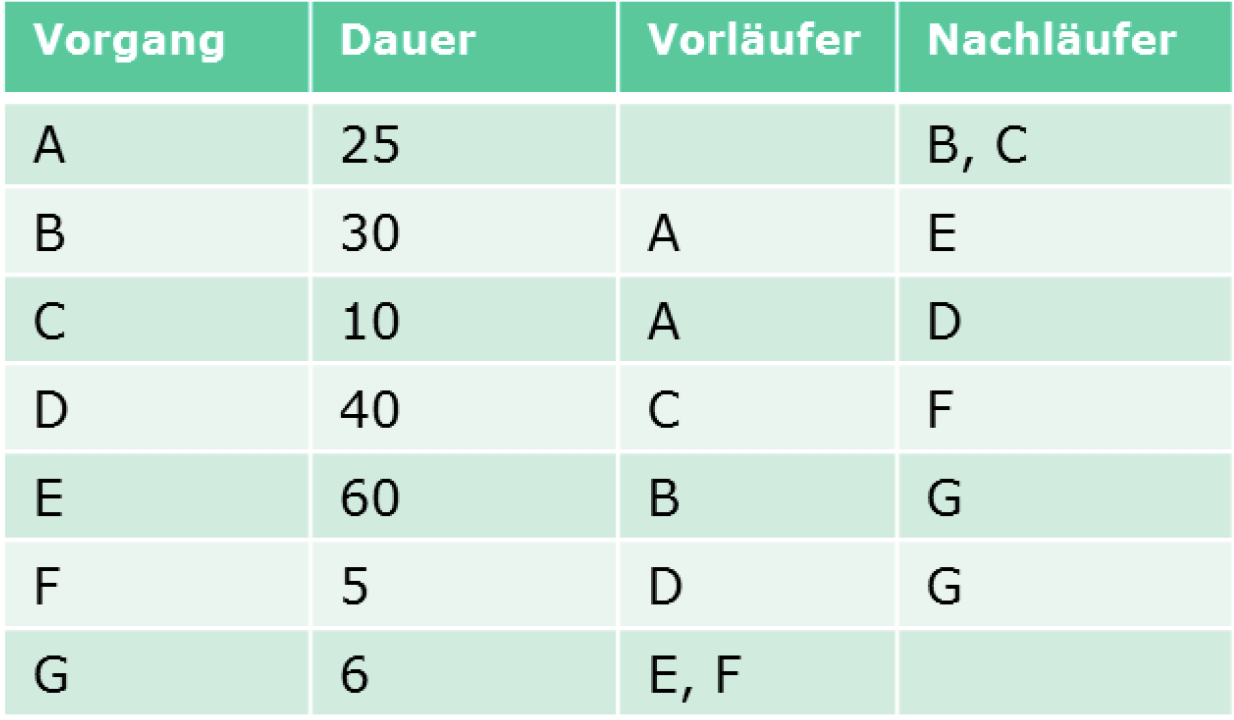
\includegraphics[height=3cm]{img/pm/cpm_vorgangsliste.png}
				\caption{Vorgangsliste}
				\label{fig:pm_cpm_vorgangsliste}
			\end{figure}
			\noindent
			In Vorgangsliste sind pro AP direkte Vorläufer \& Nachläufer aufgelistet.
			Zur Erstellung des Vorgangsdiagramm würde eines davon ausreichen.
			Daraus wird nun das Vorgangsdiagramm erstellt.
			Bei diesem fehlen jedoch noch die Zeitpunkte.
			Die Dauer der Vorgänge werden auf den Pfeilen eingetragen.
			
			\newpage
			
			\begin{figure}[!htb]
				\centering
				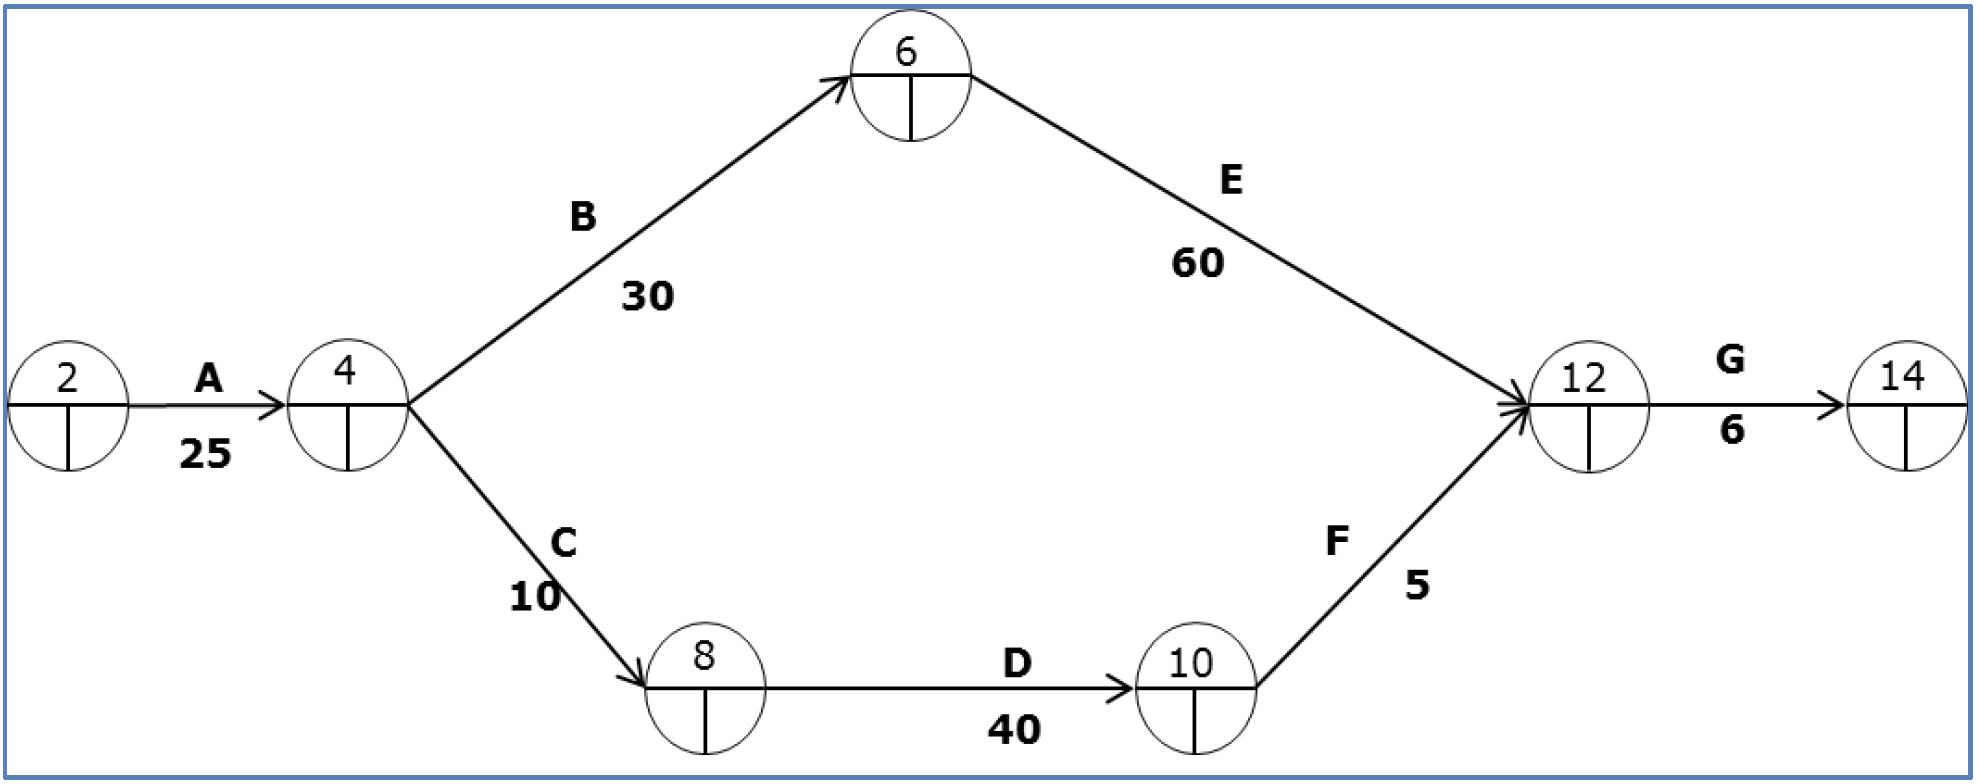
\includegraphics[height=3.5cm]{img/pm/cpm_netzplan.png}
				\caption{Vorgangspfeil-Netzplan ohne Zeitpunkte}
				\label{fig:pm_cpm_netzplan}
			\end{figure}
			\noindent
			Als Nächstes werden die \textbf{frühesten Zeitpunkte} ermittelt.\\
			\textit{(Werden 2 oder mehr Pfade zusammengeführt, wird als FA des nachlaufenden Vorgangs der höchste errechnete Wert eingefügt, da die frühest möglichen Zeitpunkte gesucht sind)}
			
			\begin{figure}[!htb]
				\centering
				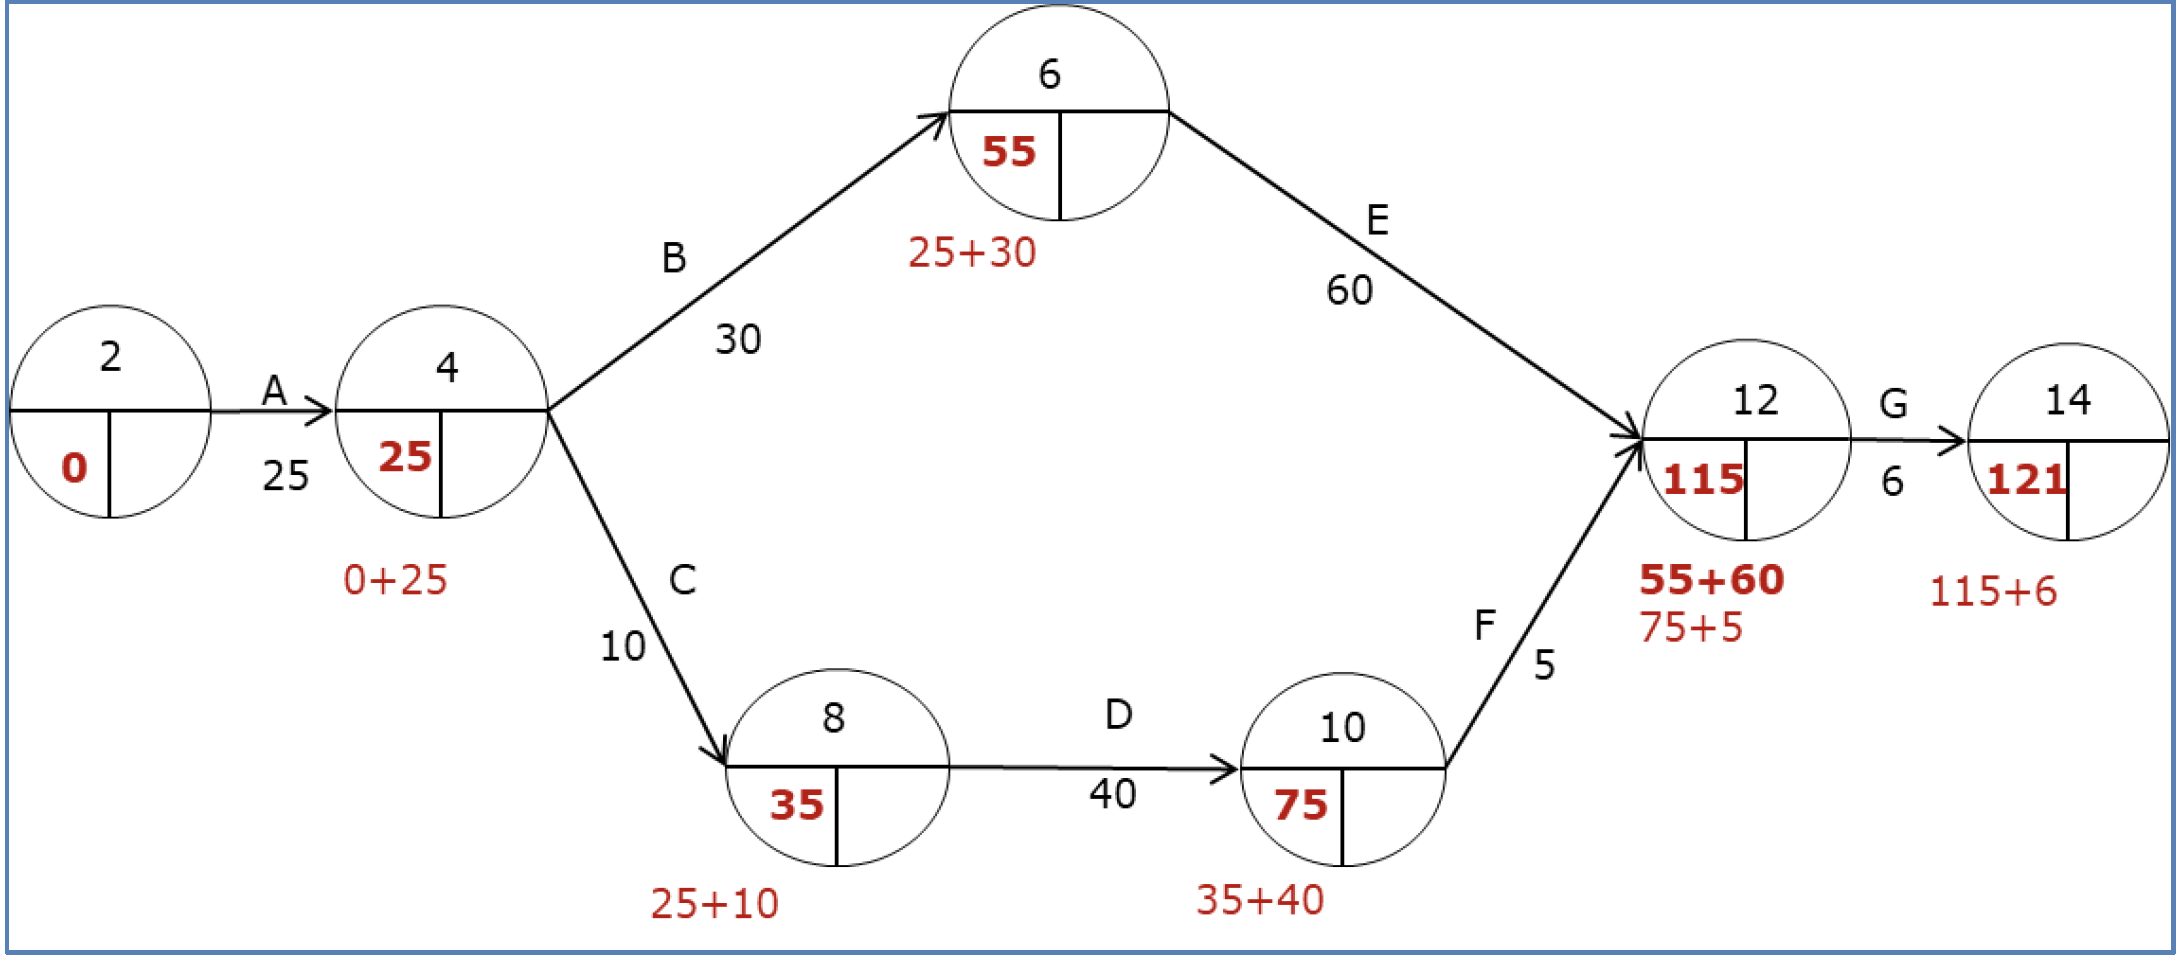
\includegraphics[height=3.5cm]{img/pm/cpm_soonest.png}
				\caption{VPN: Berechnung der frühesten Zeitpunkte}
				\label{fig:pm_cpm_soonest}
			\end{figure}
			\noindent
			Als Nächstes werden noch die \textbf{spätesten Zeitpunkte} berechnet.\\
			\textit{(Werden 2 oder mehr Pfade zusammengeführt, wird als SE des nachlaufenden Vorgangs der tiefste errechnete Wert eingefügt, da die spätest möglichen Zeitpunkte gesucht sind)}
			
			\begin{figure}[!htb]
				\centering
				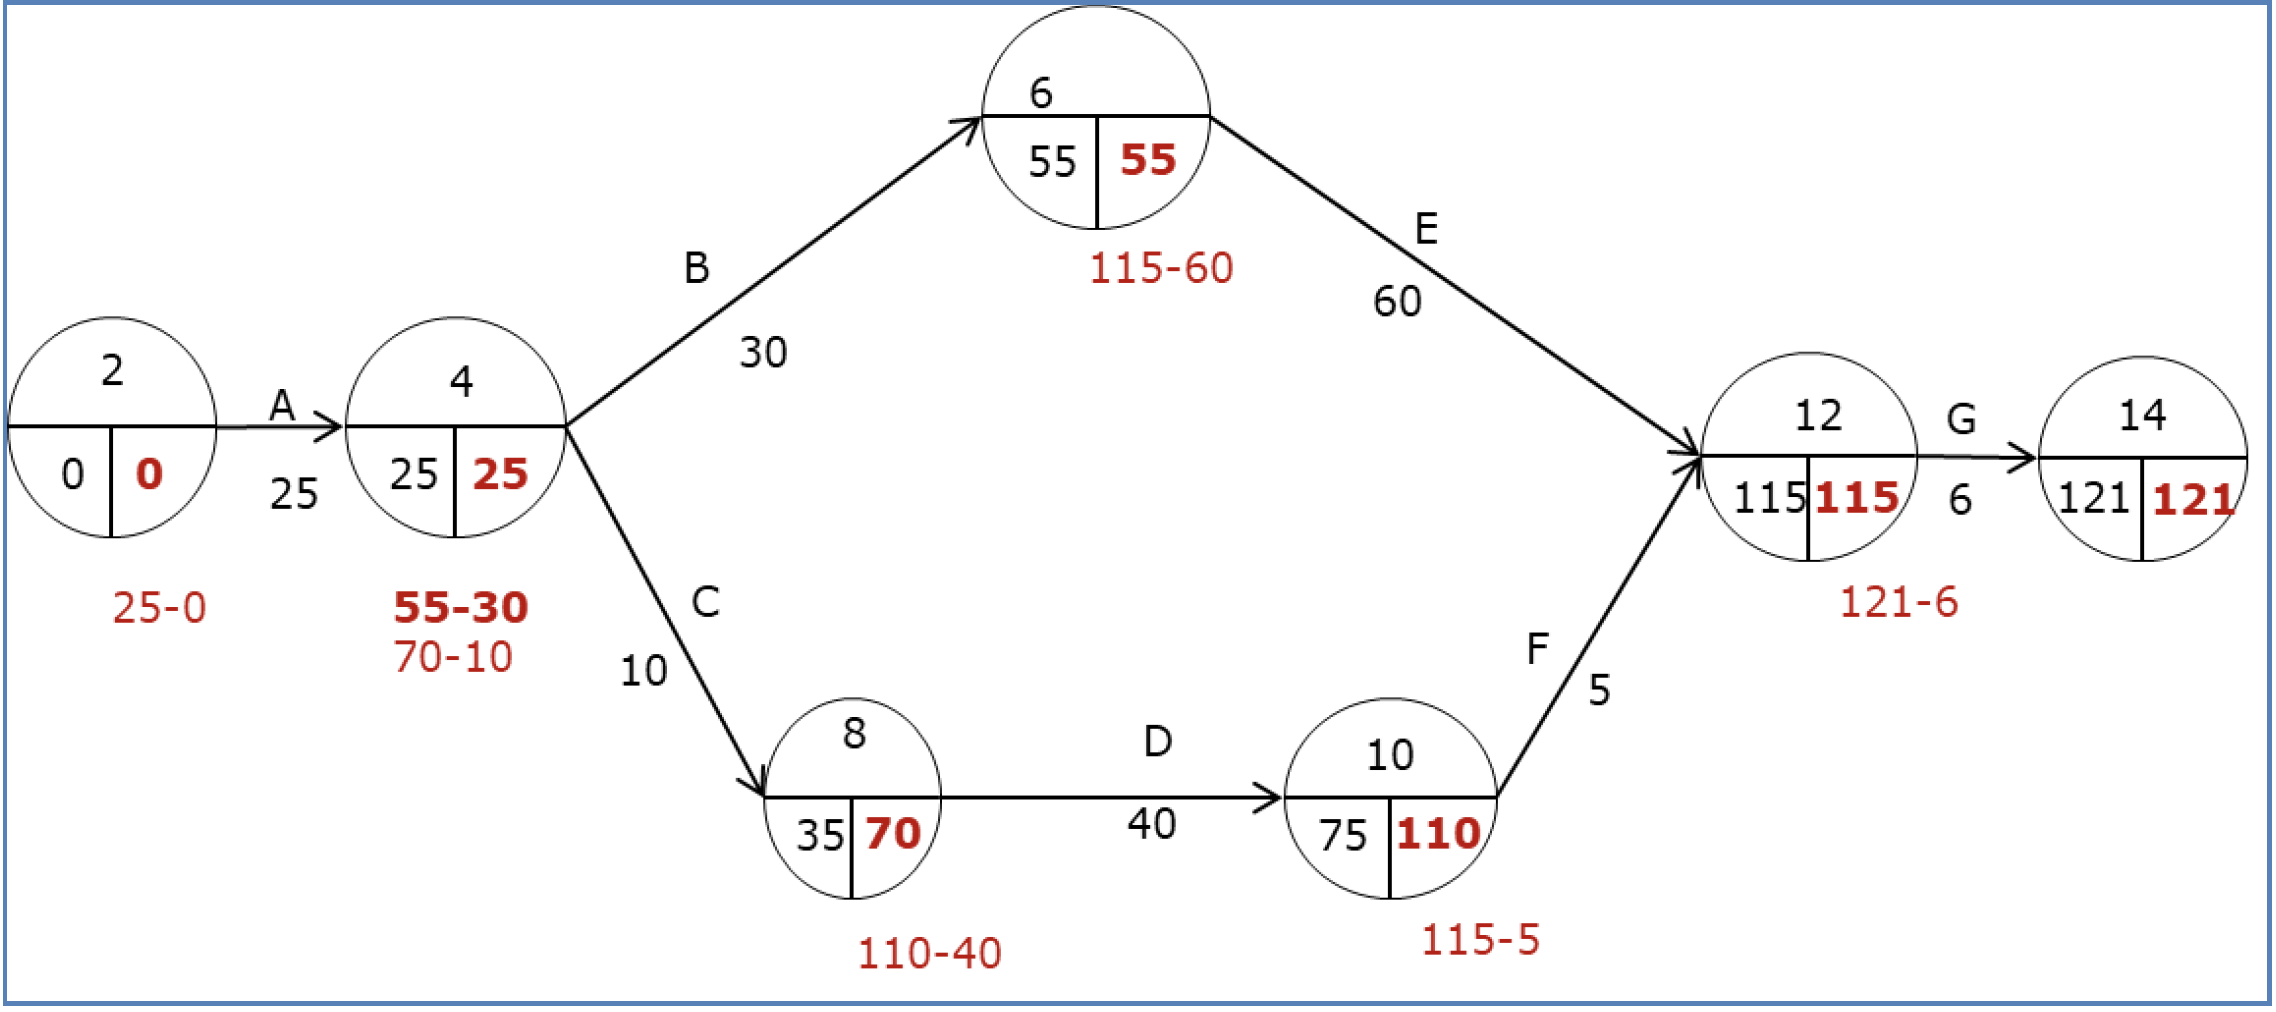
\includegraphics[height=3.5cm]{img/pm/cpm_latest.png}
				\caption{VPN: Berechnung der spätesten Zeitpunkte}
				\label{fig:pm_cpm_latest}
			\end{figure}
			\noindent
			Nun wird noch der kritische Pfad ermittelt.
			Dieser besteht aus den Vorgängen, welche keine (gesamte) Pufferzeit aufweisen (in diesem Fall A, B, E, G)
			
			\begin{figure}[!htb]
				\centering
				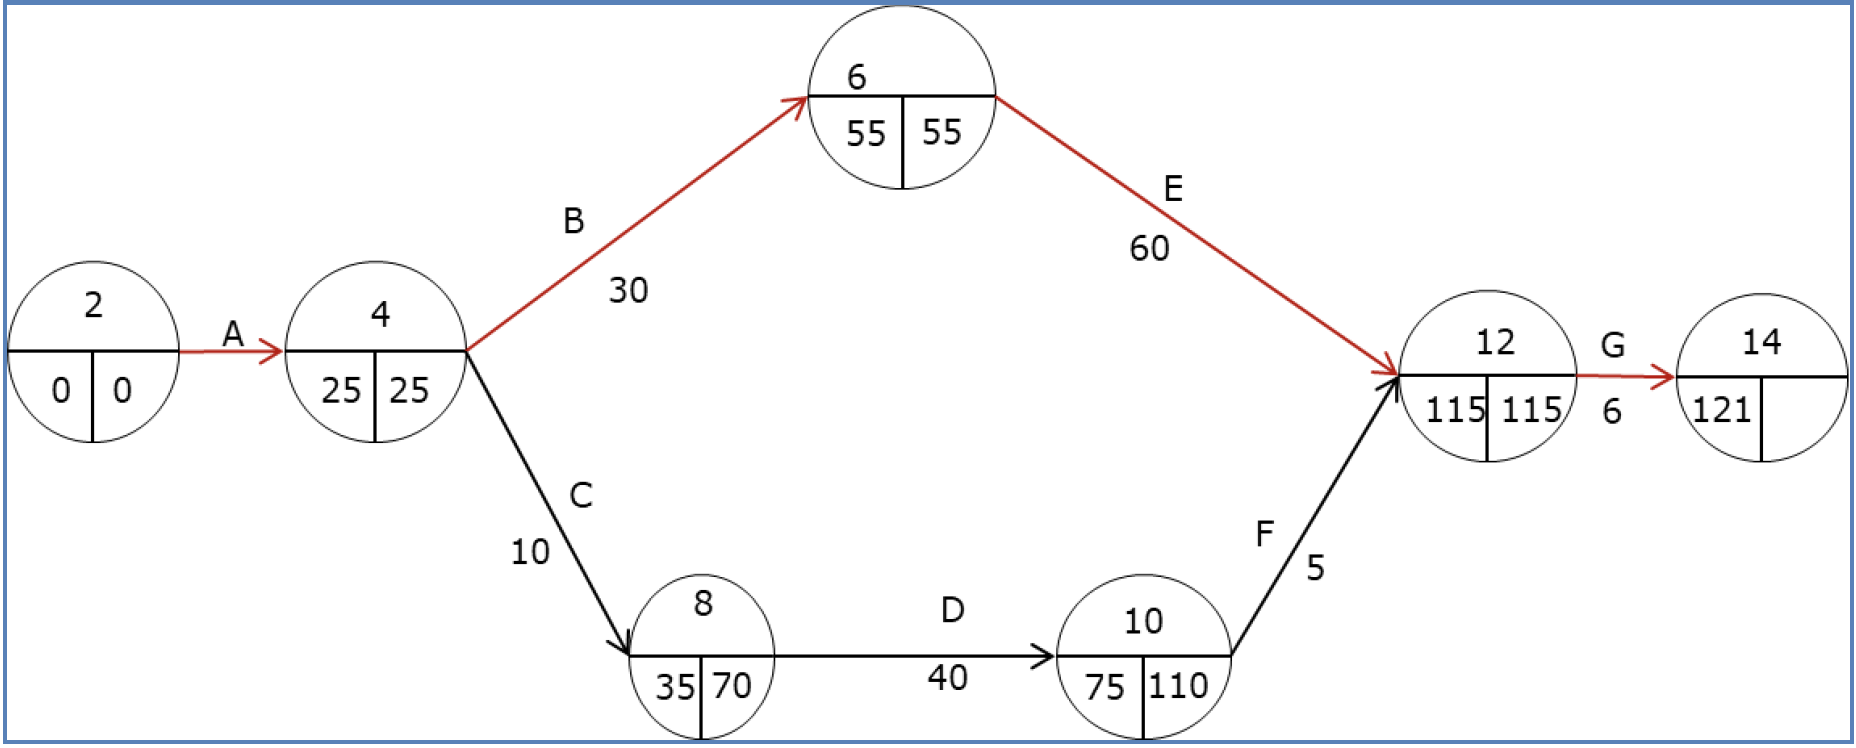
\includegraphics[height=3.5cm]{img/pm/cpm_critical.png}
				\caption{VPN: Ermitteln des kritischen Pfads}
				\label{fig:pm_cpm_critical}
			\end{figure}
		
\newpage

			\paragraph{Precedence Diagramming Method (PDM)}
			
			Findet sich in toolgestützten PM-Werkzeugen.
			Pufferzeiten werden ebenfalls durch Vorwärts- / Rückwärtsrechnung errechnet.
			
			\begin{itemize}
				\item FAZ bis FEZ: Puffer
				\item SAZ bis SEZ: Dauer des Vorgangs
			\end{itemize}
		
			\paragraph{Pufferzeiten}
			
			Pufferzeiten geben Auskunft, wie viel Reserve im Ablaufplan beinhaltet ist.
			Kritischer Pfad gibt Auskunft in welchen APs keine Reserven vorhanden sind bzw. welche Vorgangskette optimiert werden muss, um den Projektendzeitpunkt zu beeinflussen.\\
			\textit{(Aufwände \& Ressourcen/Skills in diesem Planungsstadium noch nicht berücksichtigt.
			Diese haben eine entscheidende Auswirkung auf die Dauer von APs)}
		
			\paragraph{Berechnung von Pufferzeiten}
			
			\begin{figure}[!htb]
				\centering
				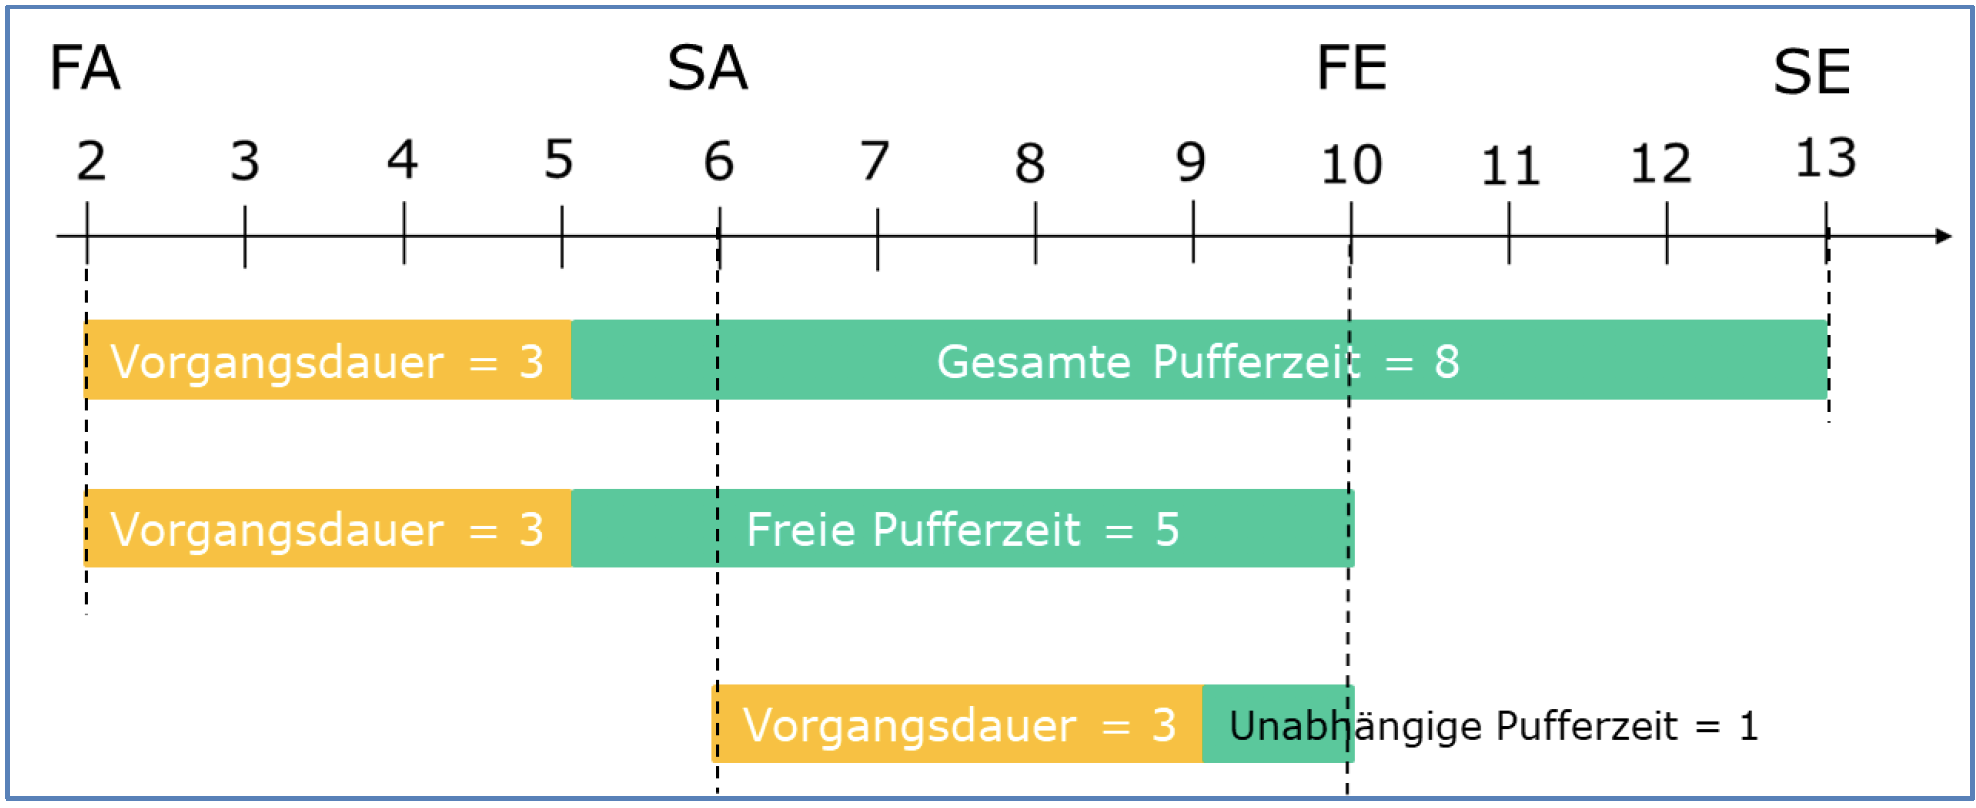
\includegraphics[height=4cm]{img/pm/pdm_pufferzeiten.png}
				\caption{Pufferzeiten nach PDM}
				\label{fig:pm_pdm_pufferzeiten}
			\end{figure}
			
			\paragraph{Gesamte Pufferzeit (GP)}
			
			\begin{quote}
				$GP = SE(B) - FA(A) - Vorgangsdauer$
			\end{quote}
			\noindent
			Gibt an, wie lange ein Vorgang bzw. sein Anfangszeitpunkt maximal ausgedehnt/hinausgezögert werden darf, ohne dass das nachfolgende AP (und Endzeitpunkt des Projekt) beeinträchtigt wird\\
			Vorgang(-skette) ist \textbf{kritisch} (auf kritischem Pfad), wenn GP = 0 ist!
			
			\paragraph{Freie Pufferzeit (FP)}
			
			\begin{quote}
				$FP = FE(B) - FA(A) - Vorgangsdauer$
			\end{quote}
			\noindent
			Gibt an, wie lange ein Vorgang bzw. sein Anfangszeitpunkt maximal ausgedehnt/hinausgezögert werden darf, ohne dass der früheste Anfangszeitpunkt des nachfolgenden Vorgangs beeinträchtigt wird
			
			\paragraph{Unabhängige Pufferzeit (UP)}
			
			\begin{quote}
				$UP = FE(B) - SA(A) - Vorgangsdauer$
			\end{quote}
			\noindent
			Gibt an, wie lange ein Vorgang bzw. sein Anfangszeitpunkt maximal ausgedehnt/hinausgezögert werden darf, ohne dass der früheste Anfangszeitpunkt des nachfolgenden Vorgangs beeinträchtigt wird - \textbf{unabhängig} darum, weil nicht relevant ist, wann das Anfangsereignis tatsächlich ausgelöst wird
			
			\paragraph{Resultat - Ablaufplan}
			
			Als Resultat dieses Planungsschrittes entsteht ein Ablaufplan, wobei bei der AP-Liste die Spalten von \textit{Vorgänge} (also \textit{Vorgangsdauer}, \textit{Direkter Vorläufer} und \textit{direkter Nachläufer}) ausgefüllt werden.
			
\newpage

			\subsubsection{Ressourcenplanung}
			
			\begin{description}
				\item[Input] Ablaufplan
				\item[Ziel] Kapazitäten SOLL vs. Kapazitäten IST, Aufwände \& Dauer ermitteln
				\item[Output] Durchlaufzeit/Dauer (Aufwand) der APs
				\item[Lieferobjekt] Ressourcenplan, Kapazitätsbelastungsdiagramm
			\end{description}
		
			\paragraph{FTE - Full Time Equivalent}
			
			\begin{itemize}
				\item Einplanung von personenneutralen Ressourcen (keine konkreten Mitarbeitenden)
				\item \textbf{1 FTE} entspricht einer Vollzeitstelle (Ein Mitarbeiter, der zu 100\% im Projekt tätig ist)\\
				(\textit{bspw. 1 FTE = 3 Mitarbeitende (1x 50\%, 2x je 25\%)})
			\end{itemize}
		
			\paragraph{Dauer / Aufwand / FTE}
			
			\begin{quote}
				Verhältnis von \textbf{FTE} zu Dauer \& Aufwand:\\
				\\
				(1) $FTE = \frac{Aufwand[Tagen]}{Dauer[Tagen]}$\\
				\\
				(2) $Aufwand[Tagen] = Dauer[Tagen] \times FTE$\\
				\\
				(3) $Dauer[Tagen] = \frac{Aufwand[Tagen]}{FTE}$		
			\end{quote}
		
			\begin{itemize}
				\item \textbf{Terminfixierte Planung}\\
						Bei personeller Ressourcenplanung ist Dauer eines AP grundsätzlich gesetzt, es sind die benötigten Ressourcen/ Personalkapazitäten (in FTE) pro AP in Abhängigkeit der Dauer \& des Aufwands gesucht. Dazu wird \textbf{Formel (1)} verwendet (Aufwand muss noch geschätzt werden)
				\item \textbf{Ressourcenfixierte Planung} (Einsatz verfügbarer personeller Ressourcen)\\
						Sind die personellen Ressourcen fix vorgegeben und der Aufwand ist klar, wird die Dauer des AP änderbar. 
						Man verwendet \textbf{Formel (3)}.
			\end{itemize}
			
			\paragraph{Aufwandschätzung / Schätztechniken}
			
			Schätzung der Aufwände sehr schwierig, Dauer eines AP oder Personaleinsatz in AP hängen davon ab.
			Aufwände bestimmen letztendlich die Durchlaufzeit \& Kosten eines AP und somit des Projekts.
			Aufwandschätzungen werden periodisch überprüft und damit im Laufe des Projektfortschritts immer genauer.
			
			\begin{quote}
				Parkinson's erstes Gesetz:\\
				\textit{Work exdpands so as to fill the time available for its completion}\\
				\textit{Arbeit dehnt sich aus, soweit es geht}
			\end{quote}
			Aus der Praxis bekannt, ist man zu früh fertig, findet man immer Arbeit zur "Verschönerung" oder testet mehr etc. $\rightarrow$ Time Boxing
			
			\paragraph{Techniken zur Aufwandschätzung}
			
			\begin{itemize}
				\item Standard Delphi-Verfahren
				\item Breitband Delphi-Verfahren
				\item Beta-Verfahren
				\item Function Point ($\rightarrow$ SW-Development)
				\item COCOMO (Constructive Cost Model); in vielen Varianten
				\item LOC (Lines of Code $\rightarrow$ SW-Development)
				\item etc.
			\end{itemize}
			
\newpage

			\paragraph{Kapazitätsbelastung (-sdiagramm)}
			
			Nachfolgende Abbilding zeigt die berechneten Ressourcen pro Arbeitspaket auf.
			
			\begin{figure}[!htb]
				\centering
				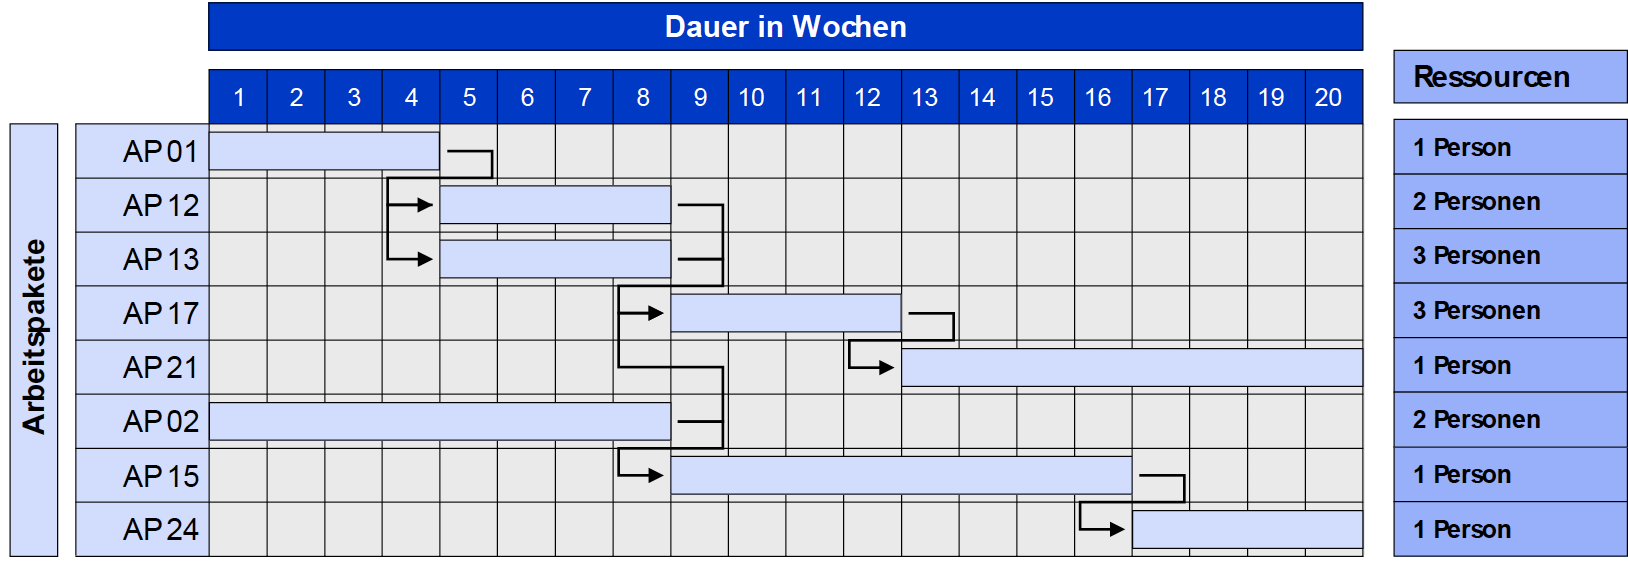
\includegraphics[height=5cm]{img/pm/belastung.png}
				\caption{Beispiel Kapazitätsbelastung}
				\label{fig:pm_belastung}
			\end{figure}
			\noindent
			Aus obiger Abbildung lässt sich nun ein Kapazitätsdiagramm erstellen, welches die notwendige Kapazität über die Projektdauer visualisiert.
			Somit wird ersichtlich, wann im Projekt wieviel Kapazität eines bestimmten Skills einer Personalressource verfügbar sein muss.
		
			\begin{figure}[!htb]
				\centering
				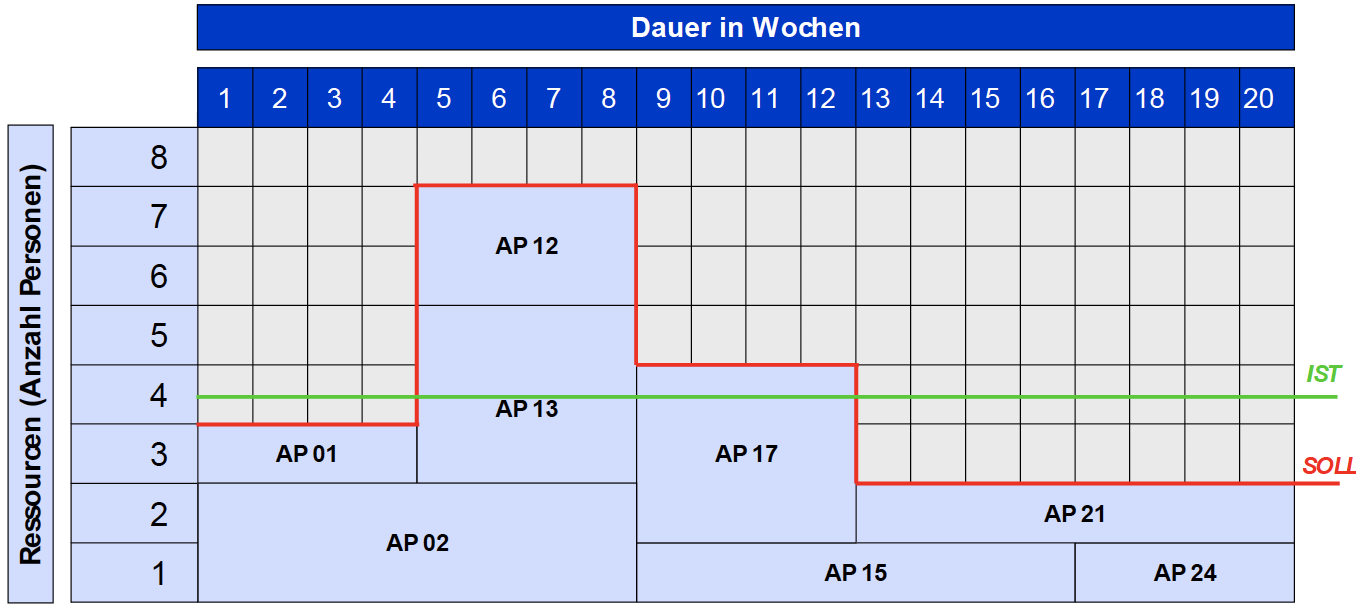
\includegraphics[height=5cm]{img/pm/belastung_dia.png}
				\caption{Beispiel Kapazitätsbelastungsdiagramm}
				\label{fig:pm_belastung_diagramm}
			\end{figure}
			\noindent
			Lustige Info: Im Skript \textit{Projekt in Gang halten} unter zugehörigem Kapitel ist eine übungsaufgabe, bei welcher mithilfe eines VPN und zugehörigen Netzplänen für frühste und späteste Lage jeweils ein Kapazitätsbelastungsdiagramm für früheste/späteste Lage erstellt wird.
			Ich bin zu müde dass jetzt noch hier reinzuklatschen.
			
\newpage

		\subsubsection{Organisationsplanung / Aufbauorganisation}
			
			\begin{description}
				\item[Input] Ressourcenplan, Projektorganisation
				\item[Ziel] Selektions Projektmitarbeitender, Überführung Ressourcenplanung in Aufbauorganisation
				\item[Output] Mitarbeitende (intern, extern) zugeteilt auf APs
				\item[Lieferobjekt] Organisationsplan
			\end{description}
			\vspace{1em}
			\noindent
			Tätigkeiten der Organisationsplanung:
			\begin{itemize}
				\item Projektmitarbeitende selektieren
				\item Projektorganisation initialisieren
				\item Stellebeschriebe $\rightarrow$ AKV : Aufgabe, Kompetenz, Verantwortung
				\item Arbeitspakete an Projektmitarbeitende zuordnen
			\end{itemize}
		
			\paragraph{Projektorganisationen}
			
			3 verschiedene Projektorganisationsarten:
			
			\begin{figure}[!htb]
				\centering
				\begin{subfigure}{.45\textwidth}
					\centering
					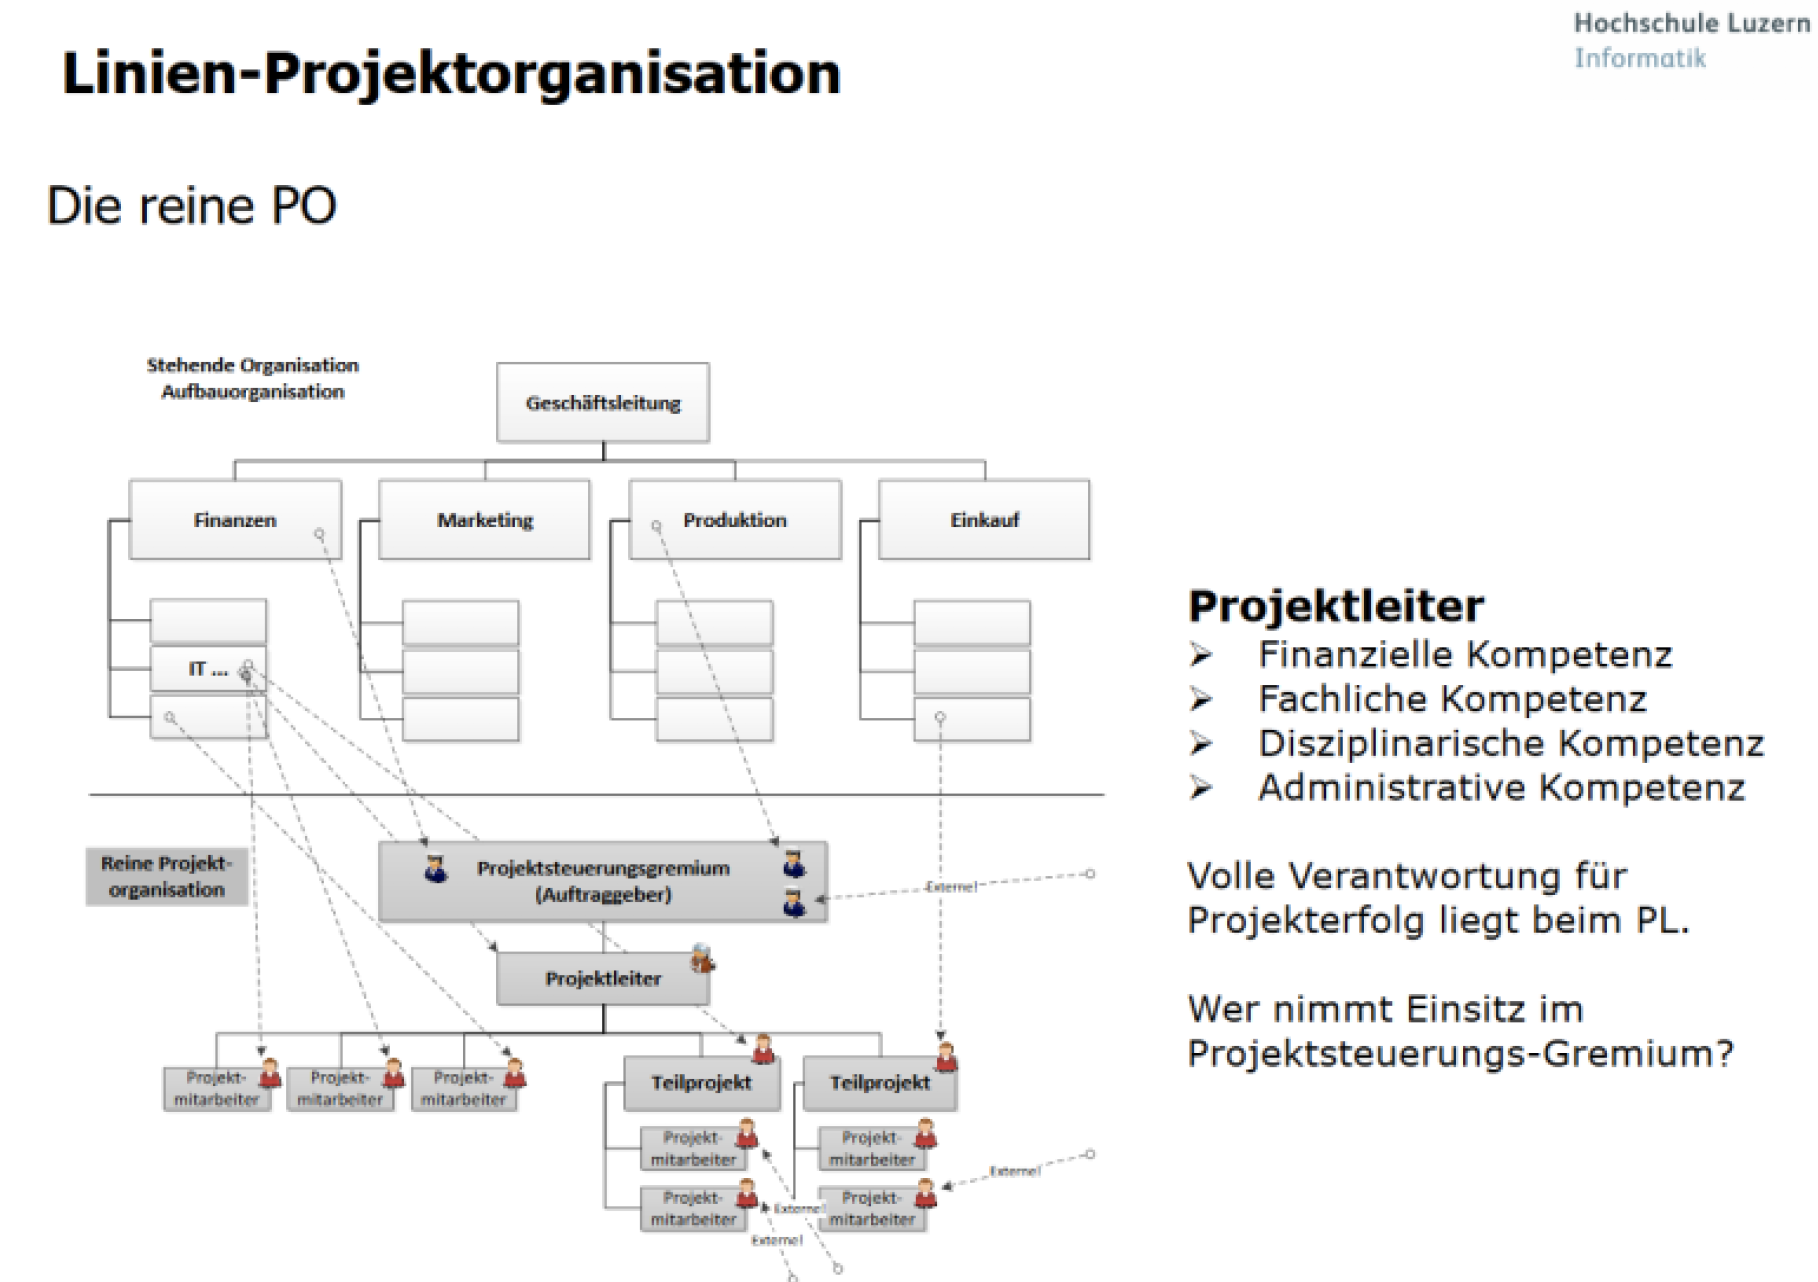
\includegraphics[height=4.5cm]{img/pm/po_linien.png}
					\label{fig:pm_po_linie}
				\end{subfigure}
				\begin{subfigure}{.45\textwidth}
					\centering
					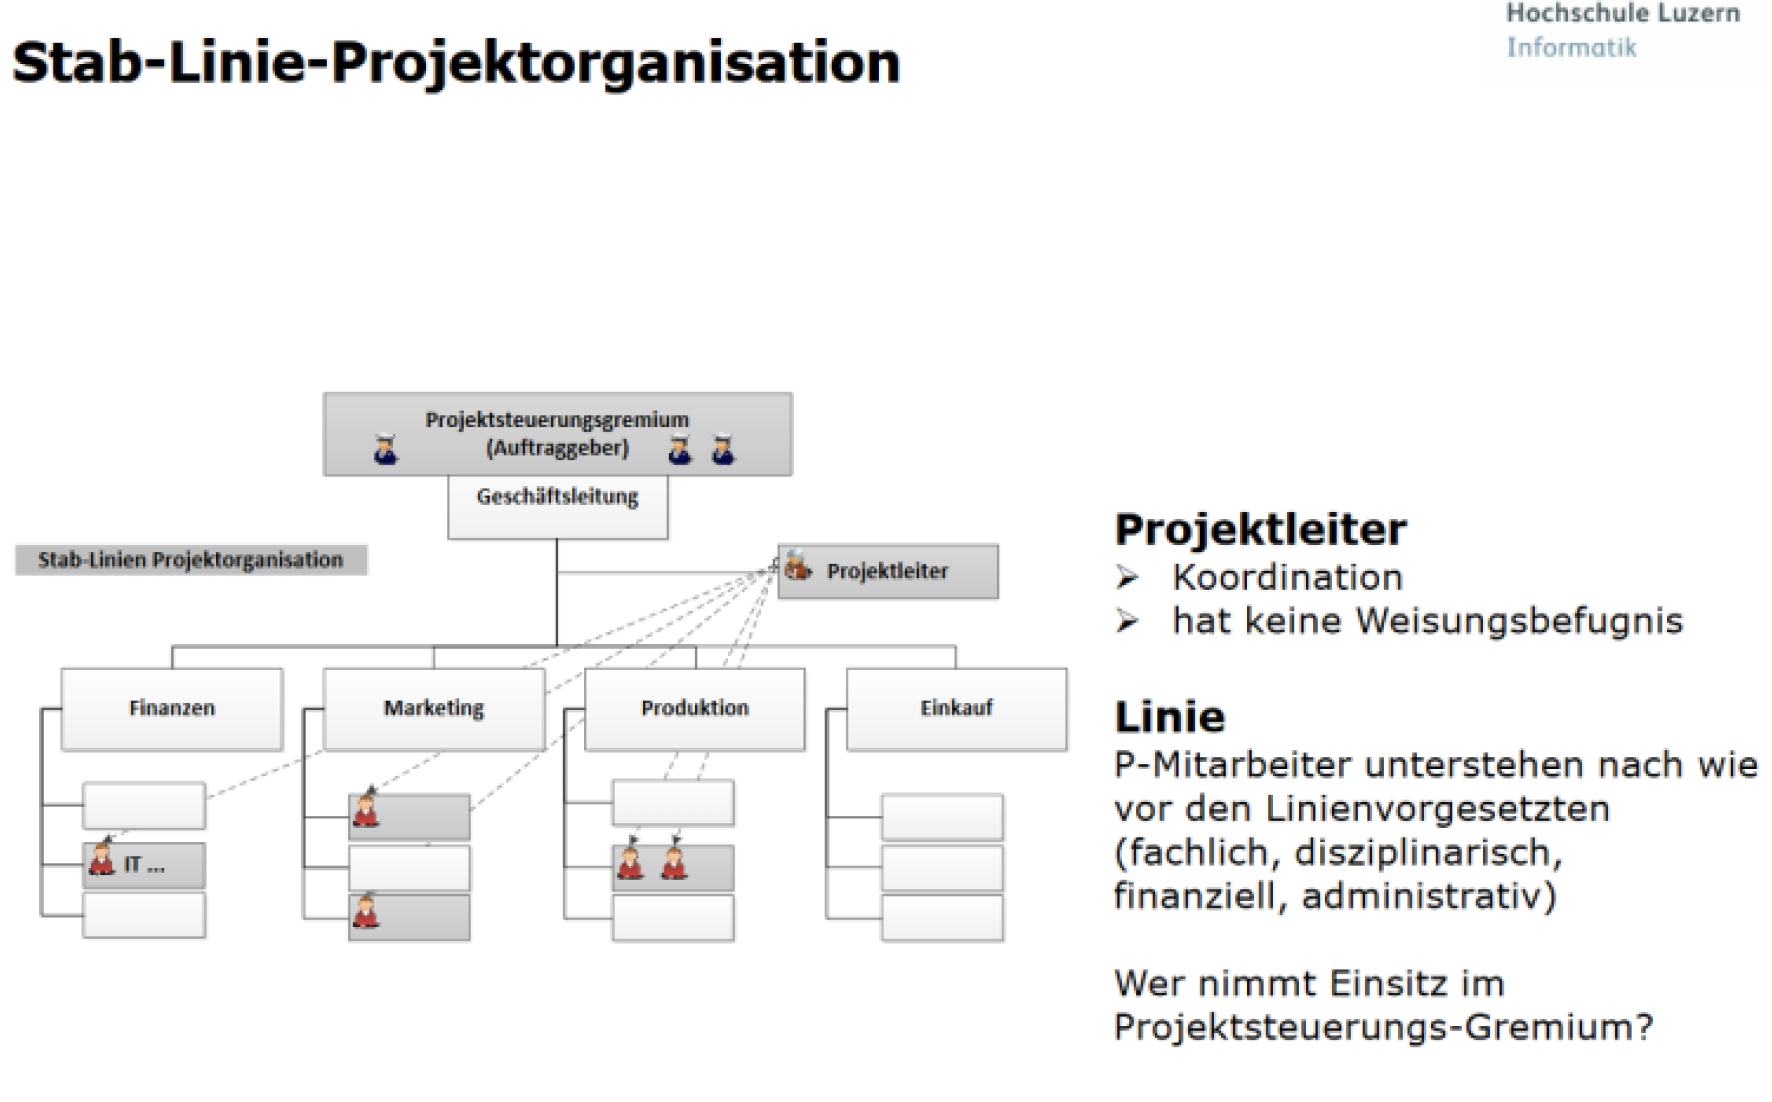
\includegraphics[height=4.5cm]{img/pm/po_stablinie.png}
					\label{fig:pm_po_stablinie}
				\end{subfigure}
			\end{figure}
		
			\begin{figure}[!htb]
				\centering
				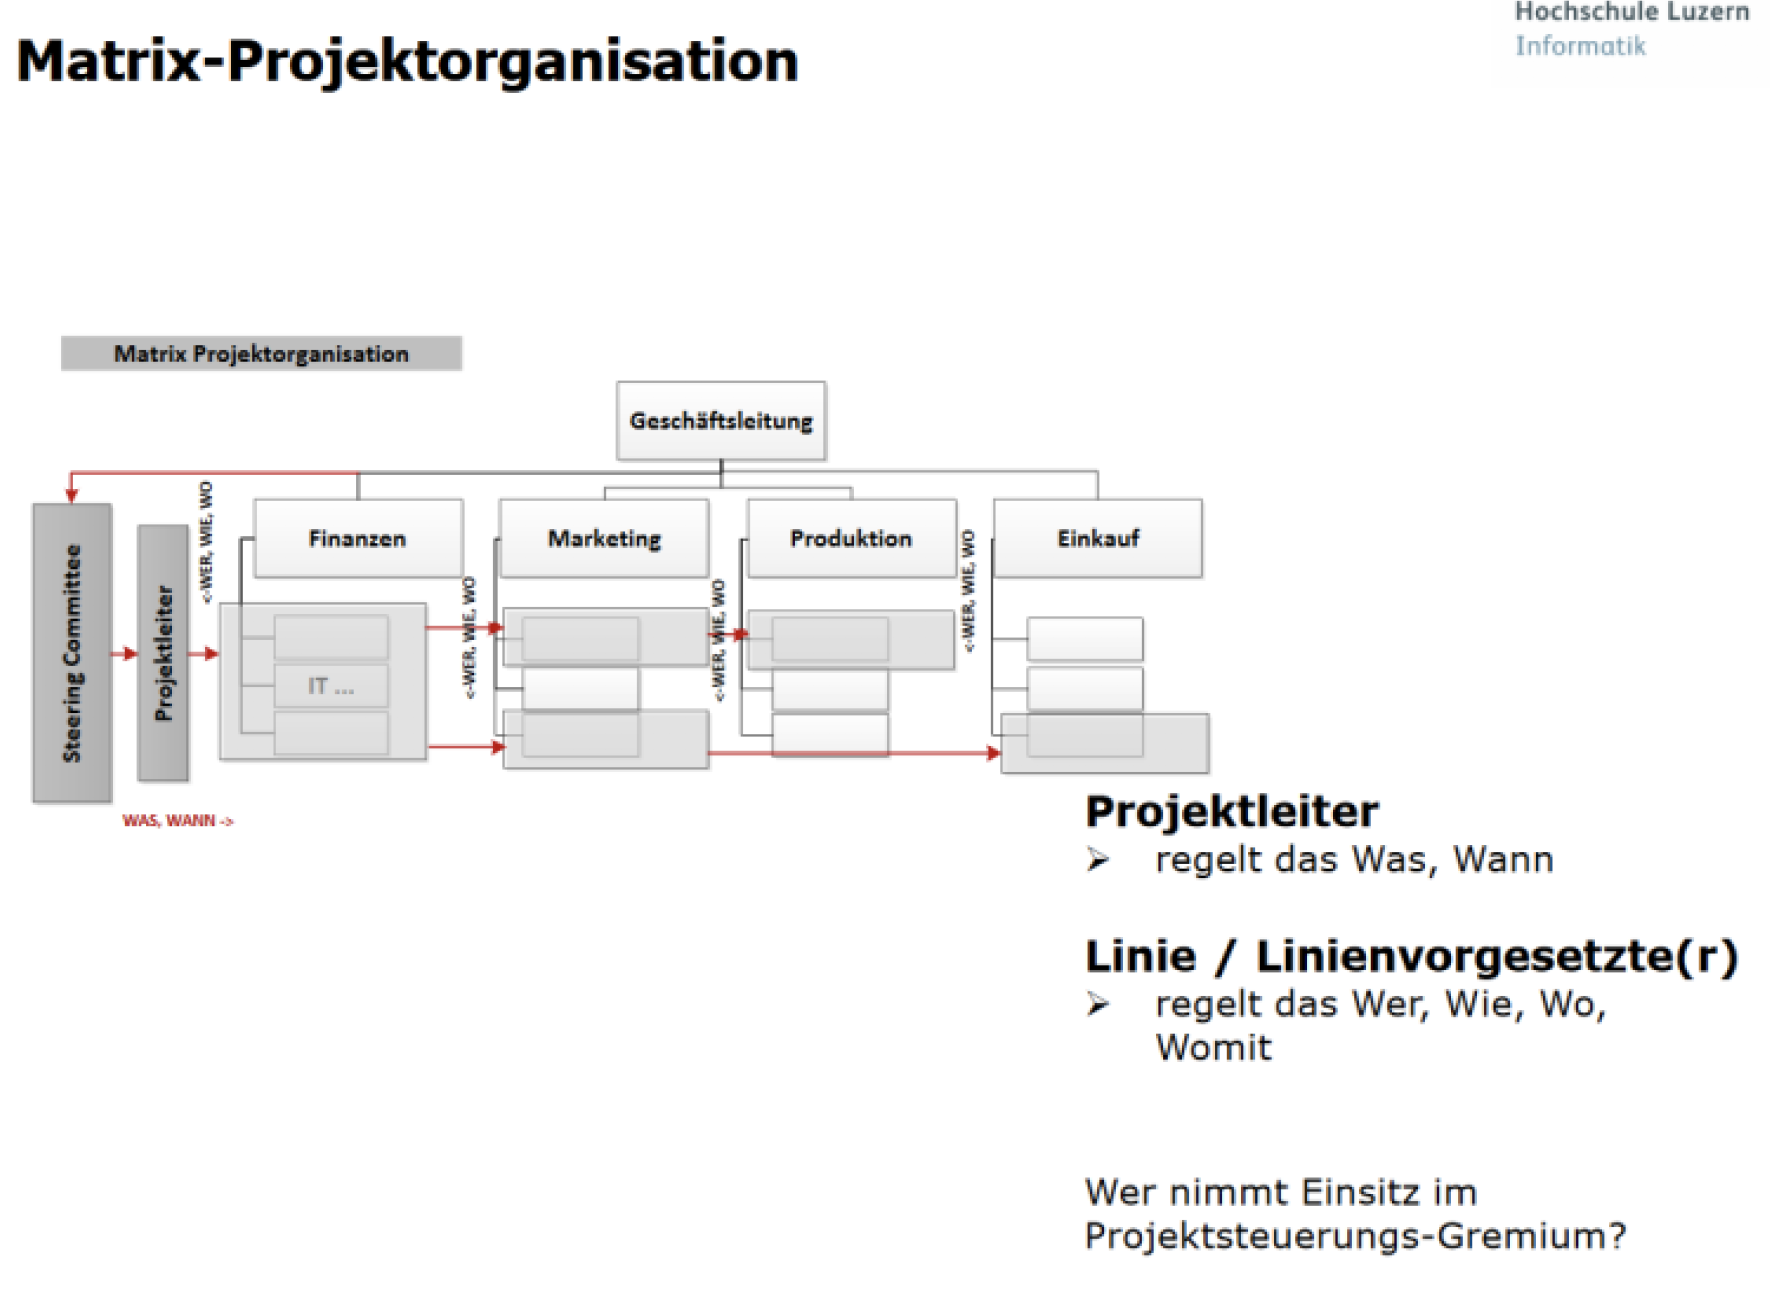
\includegraphics[height=5cm]{img/pm/po_matrix.png}
				\label{fig:pm_po_matrix}
			\end{figure}
		
			\paragraph{Optimale Teamgrösse}
			
			Optimale Teamgrösse basierend auf der Anzahl Kommunikationsbeziehungen in einer Gruppe.
			
			\begin{itemize}
				\item Pro Kommunikationsbeziehung: wöchentlicher Zeitverlust von 40 Minuten pro Mitarbeiter
				\item Arbeitszeit pro Woche \& MA = 40 Stunden
				\item \#MA = Anzahl Mitarbeiter
			\end{itemize}
		
			\begin{quote}
				$Dauer[Tage] = \frac{Aufwand[Tage]}{\#MA}$\\
				\\
				$Dauer = \frac{1}{\#MA} \times Aufwand$\\
				\\
				$Dauer = \frac{1}{\#MA \times Produktivitaet} \times Aufwand$ (Produktivität des MA berücksichtigt)
			\end{quote}
		
\newpage

			\begin{figure}[!htb]
				\centering
				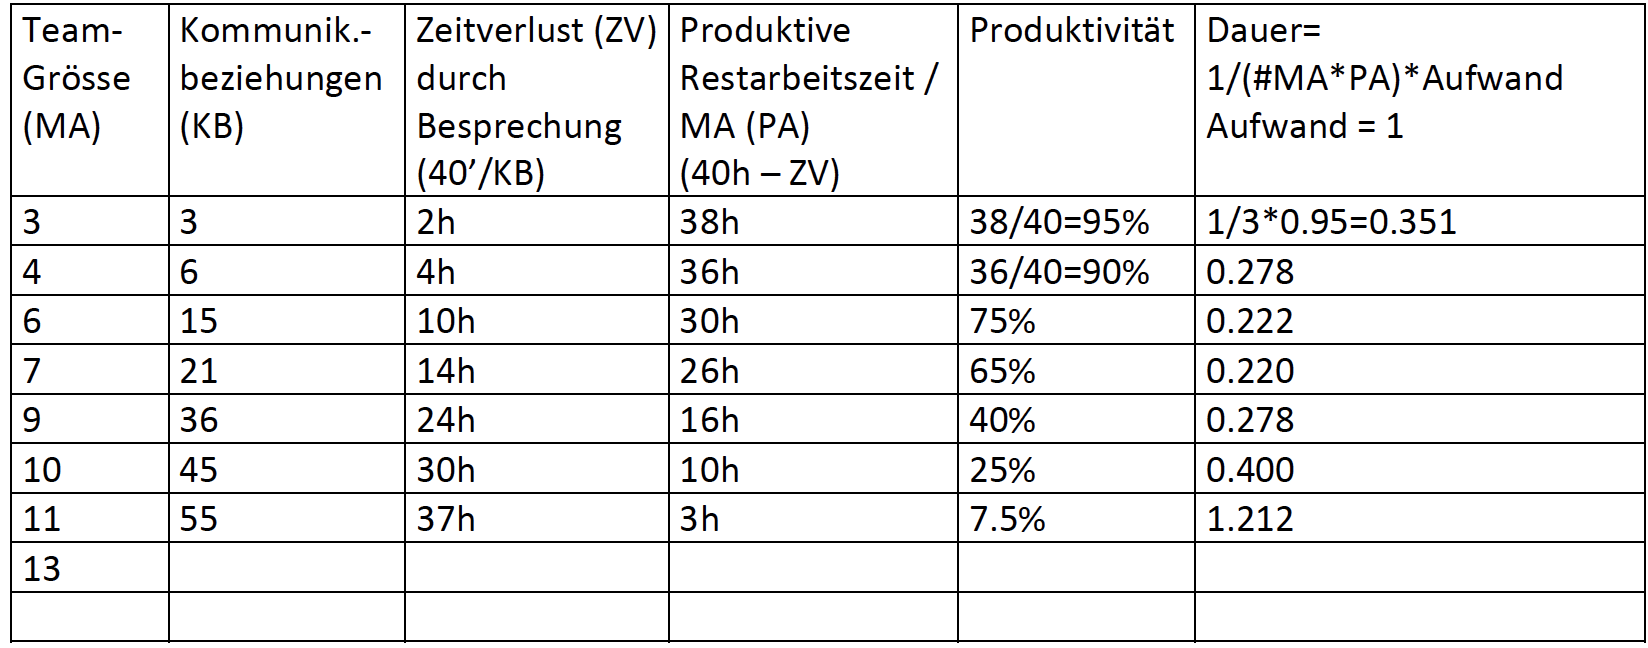
\includegraphics[height=4cm]{img/pm/opt_team.png}
				\caption{Tabelle zur Berechnung der optimalen Teamgrösse}
				\label{fig:pm_opt_team}
			\end{figure}
			\noindent
			Aus der Tabelle ist ersichtlich: Bei einer Teamgrösse von 7 zeigt die Berechnung der Dauer einen Minimalwert von 0.22 $\rightarrow$ die kürzeste Dauer
			
		\subsubsection{Projektkostenplanung}
		
		\begin{description}
			\item[Input] Organisationsplan, Ressourcenplan
			\item[Ziel] Ermittlung, Optimierung \& Finanzierung der im Projekt anfallenden Kosten
			\item[Output] Dokumentierte Kosten und deren Finanzierung
			\item[Lieferobjekt] Projektkostenplan
		\end{description}
		\vspace{1em}
		\textbf{Projektkosten} werden die im Projekt anfallenden Kosten für das gesamte Projekt bzw. für die Gesamtheit aller AP verstanden.\\
		\textbf{Betriebskosten}, welche nach Einführung anfallen, sind nicht Bestandteil der Projektkosten, müssen jedoch im Business Case aufgeführt sein.
		
		\begin{itemize}
			\item Fragen, die in \textbf{diesem Planungsschritt} beantwortet werden:
				\begin{itemize}
					\item Was kostet das Projekt?
					\item Welche Verluste fallen an, wenn das Projekt nach Konzeption/Realisierung/Einführung gestoppt wird ($\rightarrow$ Ausblick auf Projektbudgetplan)?
					\item Welche Kosten fallen intern/extern an?
					\item Welche Kosten sind Investitionen, die amortisiert werden müssen?
					\item Welche der möglichen Lösungsvarianten ist kostenmässig optimal (Kostenvergleichsrechnung)?
				\end{itemize}
			\item Fragen, die in einem Business Case beantwortet werden müssen:
				\begin{itemize}
					\item Was ist der Nutzen des Projekts? $\rightarrow$ Business Case
					\item Was sind die Folgekosten ($\rightarrow$ Nutzungsphase) des Projekts?
					\item Welche Lösungsvariante ist über die gesamte Lebensdauer die Optimale (Kosten-Nutzen)?
				\end{itemize}
		\end{itemize}
	
			\paragraph{Kostenarten \& Kostenstruktur}
			
			Mögliche Projektkosten:
			
			\begin{itemize}
				\item Interne Personalkosten
				\item Externe Personalkosten
				\item Material (HW, SW)
				\item Temporäre Mieten für Räumlichkeiten
				\item Interne Kosten für Bereistellung \& Betrieb von Testsystemen
				\item Zusätzliche Lizenzkosten pro-rata während Projektdauer
				\item etc.
			\end{itemize}
			\vspace{1em}
			\noindent
			Möglichkeiten für die Strukturierung der obigen Kostenarten:
			
			\begin{itemize}
				\item \textit{Ausgabenwirksame Kosten vs. Interne Kosten:}\\
				\textbf{Ausgabenwirksame Kosten}, die ohne Projekt nicht angefallen wären, bewirken einen Mittelabfluss.
				(bspw. Kosten für externe Projekt-MAs oder Investitionen)\\
				\textbf{Interne Kosten} fallen nur kalkulatorisch an, sie fallen auch ohne Projekt an.
				(bspw. Kosten für interne Projekt-MAs, Umlagen anderer OEs auf Projekt o.ä.)
				
				\item \textit{Kosten vs. Investitionen:}\\
				\textbf{Kosten}, die während Projekt anfallen, beeinflussen Erfolgsrechnung, wobei \textbf{Investionen} aktiviert werden ($\rightarrow$ Anlagevermögen), sind somit bilanzwirksam und werden über bestimmte Zeitdauer abgeschrieben.
			\end{itemize}
			
\newpage

			\paragraph{Kosten-Nutzen-Betrachtungen: Business Case (BC)}
			
			\begin{itemize}
				\item \textit{Projektkostenplanung} kann auch für Erarbeitung/Verfeinerung des BC genutzt werden
				\item Im BC wird direkter/indirekter, der (nicht) quantifizierbare Nutzen eines Projekts ausgewiesen
				\item BC betrachtet neben Projektphase auch explizit die Nutzungsphase\\
				(Gesamt-Lifecycle eines Systems)
				\item Positiver BC is die unternehmerische Rechtfertigung für das Projekt!
				\item Direkter Nutzen:
					\begin{itemize}
						\item Direkte Einsparungen
						\item Vermeidung von Kosten
						\item Erhöhung von Einnahmen
						\item Nicht quantifizierbarer Nutzen
						\item etc.
					\end{itemize}
				\item Indirekter Nutzen:
					\begin{itemize}
						\item Technische Vorteile
						\item Marktauftritt
						\item etc.
					\end{itemize}
			\end{itemize}
		
			\paragraph{Variantenberechnungen}
			
			\begin{itemize}
				\item Eine oder mehrere grobe Varianten einer Lösung vorhanden
				\item Erste Variantenberechnungen durchführbar, Vergleich dieser wird möglich
				\item Behandelte Variante: \textbf{Statische Kostenvergleichsrechnung}
			\end{itemize}
		
			\paragraph{Statische Kostenvergleichsrechnung}
			
			\begin{itemize}
				\item Statische Methode, ermöglicht Kostenvergleich über gewisse Zeitperiode (üblich 1 Jahr)\\
					\textit{bspw. zwischen bisherigem \& neuem System oder zwei neuen Systemen (Variante A \& B)}
				\item Nur Kosten berücksichtigen, keine Erlöse\\ 
				$\rightarrow$ beide Varianten haben denselben angenommenen Erlös / Nutzen
			\end{itemize}
		
			\begin{figure}[!htb]
				\centering
				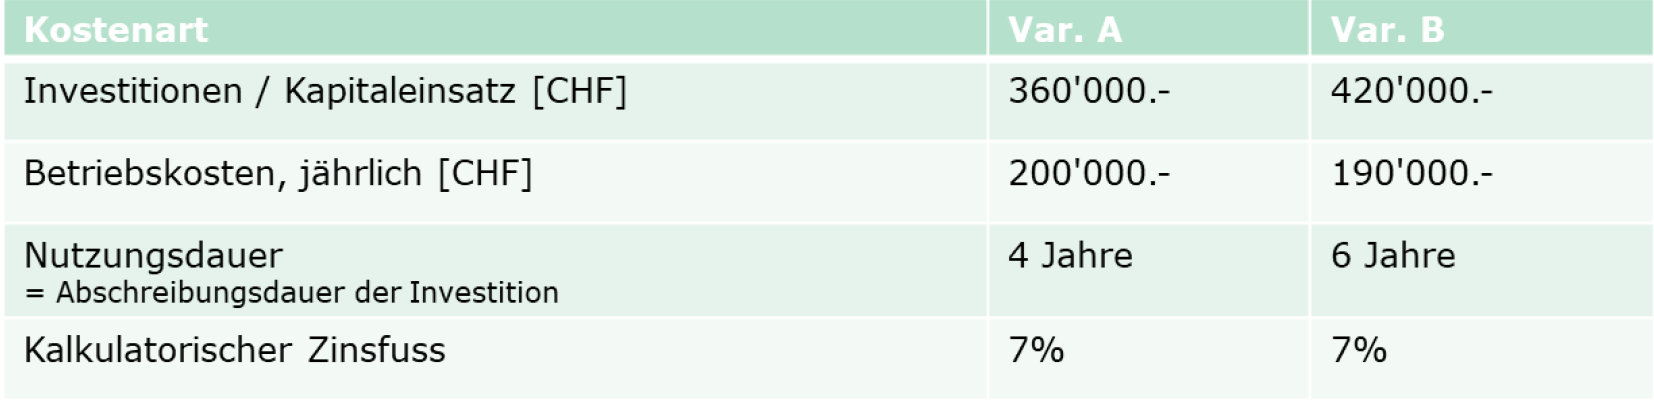
\includegraphics[height=3cm]{img/pm/kosten.png}
				\caption{Kostenvergleich zwischen Variante A und B}
				\label{fig:pm_kosten}
			\end{figure}
			\noindent
			Welche der beiden Varianten hat die tieferen jährlichen Gesamtkosten? \textbf{(Jahrl. GK)}\\
			Jährliche Gesamtkosten \textbf{GK} setzen sich zusammen aus
			\begin{description}
				\item[JB] jährliche Betriebskosten
				\item[JA] jährliche Abschreibungen (auf getätigte Investitionen)
				\item[Z] jährliche Zinskosten
			\end{description}
		
			\begin{quote}
				$Jahrl. GK = JB + JA + Z$
			\end{quote}
			
			\textbf{JB} sind Kosten, die für die Aufrechterhaltung des betriebsanfallen (bspw. Personalkosten, Strom, Räume, Wartung etc.)\\
			$\rightarrow$ im Beispiel: CHF 200'000 / CHF 190'000\\
			\\
			\textbf{JA} Abschreibungen berechnen sich aus Investitionen/Kapitaleinsatz dividiert durch Abschreibungsdauer (fixe Dauer, manchmal gleichgesetzt mit Nutzungsdauer).\\
			$\rightarrow$ im Beispiel: $\frac{CHF 360'000}{4}$ = CHF 90'000 / $\frac{CHF 420'000}{6}$ = CHF 70'000\\
			\\
			\textbf{Z} Jährlicher Zins wird auf Basis des eingesetzten Durchschnittkapitals ($\frac{Investition}{2}$) und dem kalkulatorischen Zinsfuss (durch CFO festgelegt) errechnet.\\
			$\rightarrow$ im Beispiel: $\frac{CHF 360'000}{2} \times 7 \%$ = CHF 12'600 / $\frac{CHF 420'000}{2} \times 7 \%$ = CHF 14'700
			
\newpage
			
			\begin{figure}[!htb]
				\centering
				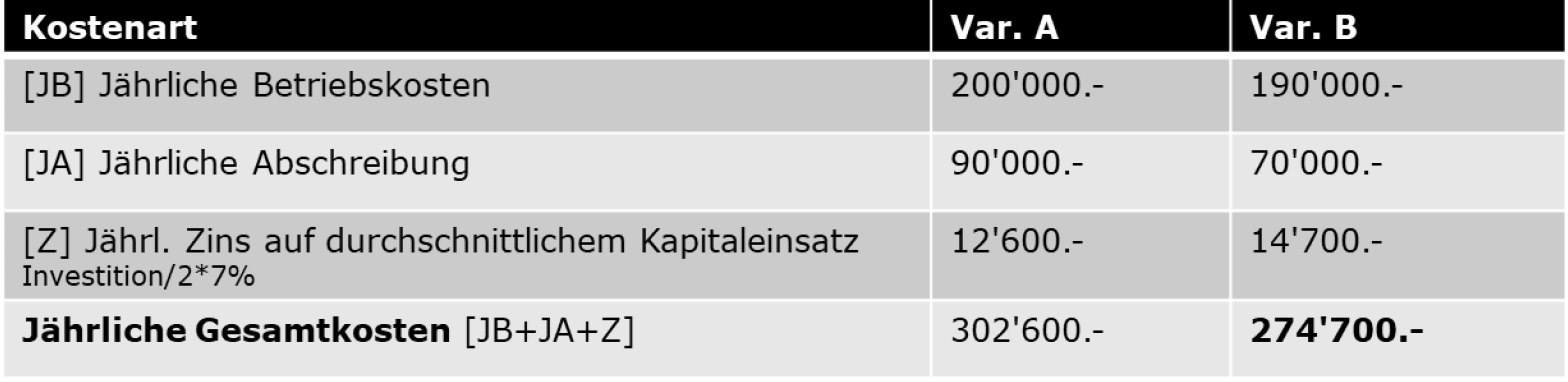
\includegraphics[height=3cm]{img/pm/kosten_result.png}
				\caption{Jährliche Gesamtkosten der Variante A und B}
				\label{fig:pm_kosten_result}
			\end{figure}
			\noindent
			\textbf{Hinweis:} Das Resultat gilt für Jahr 1 bis 4, ab Jahr 5 muss Var. A durch eine neue Lösung ersetzt sein.
			
		\subsubsection{Terminplanung}
		
		\begin{description}
			\item[Input] Ablaufplan, Projektkostenplan
			\item[Ziel] Festlegung von Terminen (kalendarisch) für Meilensteine und APs (Start, Ende)
			\item[Output] Konkrete Termin- und Einsatzplanung
			\item[Lieferobjekt] Terminplan
		\end{description}
	
		Bisher flossen zeitliche Aspekte ein, es gab jedoch noch kein "Mapping" auf kalendarischer Ebene.
		Bisheriger Plan wird auf Kalender gesetzt, Woche 1 erhält einen konkreten Starttermin.
		Es kommt zu \textbf{Planungsiterationen}: Zugeteilte Mitarbeiter sind abwesend, Auftraggeber nicht mehr zufrieden mit Wunschtermin etc.\\
		Nach Terminplanung muss oft gesamte Planung (Aufwände, Ressourcen, Dauer) neu aufgesetzt werden, um obige Ansprüche zu berücksichtigen.
		Planungstools sind hier von Vorteil.
		
		\subsubsection{Projektbudgetplanung}
		
		\begin{description}
			\item[Input] Projektkostenplan, Terminplan
			\item[Ziel] Abstimmung/Aufteilung Projektkosten auf effektiv verfügbare (finanzielle) Mittel\\
					und eventuelle Budgetrestriktionen
 			\item[Output] Kalendarische Finanzierung
			\item[Lieferobjekt] Projektbudgetplan
		\end{description}
		\vspace{1em}
		\noindent
		Planung der Projektkosten mit effektiv (im Unternehmen) vorhandenen Mitteln abgeglichen.\\
		\textbf{Budgetrestriktionen}, vorallem wenn ein Projekt über Rechnungsabschluss (Jahresende) dauert, können in diesem Planungsschritt eruiert \& gelöst werden.
		Einbezug der Finanzabteilung ist entscheidend.\\
		Alle Projekt- und Folgekosten müssen in entsprechenden Budgets berücksichtigt sein.
		Vorallem Folgekosten fallen meist in den Kostenstellen der stehenden Organisation an, nicht in dedizierten Projektkostenstellen.\\
		Budgetplanung stellt zudem sicher, dass bei Projekt, welches über das Jahresende hinweg läuft, korrekte Kosten in den richtigen Jahren budgetiert werden.
		Diese Kosten fallen ebenfalls in stehender Organisation an und müssen von Kostenstellenleitern in deren Budget berücksichtigt werden (Projektleiter hat Bring-Schuld!)\\
		Budgetprozess für neues folgendes Jahr startet oft bereits Ende Sommer des laufenden Jahres (Vorlaufzeigen), was die Projektbudgetplanung weiter erschwert.
		
\newpage
		
		\subsubsection{Informationsplanung}
		
		\begin{description}
			\item[Input] Organisationsplan, Terminplan
			\item[Ziel] Sicherstellung der Versorgung aller Stakeholder mit relevanten Infos \& Dokumentation
			\item[Output] Kommunikations- \& Informationskonzept
			\item[Lieferobjekt] Informationsplan, Dokumentationsplan
		\end{description}
	
		\paragraph{Informationsplan}
		
		Klarheit darüber, wann wer welche Informationen über welche Kommunikationskanäle in welcher Form zur Verfügung gestellt bekommt (\textbf{"push"}). Sollte folgende Spalten enthalten:
		
		\begin{itemize}
			\item \textbf{Was} (Fortschrittsbericht monatlich, Requirements Katalog präsentieren etc.)
			\item \textbf{Verantwortliche Person} (Projektleiter etc.)
			\item \textbf{Wann} (Anfangs nächsten Monat, 5.3.2017 etc.)
			\item \textbf{Form} (Bericht, Präsentation etc.)
			\item \textbf{Empfänger} (Steuerungskomitee, Teilprojektleiter, Power User etc.)
			\item \textbf{Kanal} (Email, Meeting etc.)
		\end{itemize}
		
		\paragraph{Dokumentationsplan}
		
		Zu klärende Fragen:
		
		\begin{itemize}
			\item \textbf{Dokubedürfnisse:}\\
			Was und für wen muss dokumentiert werden?
			\item \textbf{Dokuzeitpunkt:}\\
			Wann muss dokumentiert werden? Wie langt gilt eine Aufbewahrungspflicht?
			\item \textbf{Doku-Art / Doku-Träger:}\\
			Wie muss dokumentiert werden? Wo wird die Doku aufbewahrt?\\
			
			\item Kategorien im Dokumentenplan:
				\begin{itemize}
					\item Abwicklungsdokumentation (Projektauftrag, Phasenabnahmen etc.)
					\item Benutzerdokumentation (Benutzerhandbuch, Krisenplan etc.)
					\item Wartungs-/Betriebsdokumente (Systemarchitektur, Systembeschrieb etc.)
				\end{itemize}
			\item Spalten für Dokumentenplan:\\
			Dok-Nr., Dokumentationsart, Erstellzeitpunkt, Träger, Aufbewahrungsort
		\end{itemize}
		
\newpage
		
	\section{Project Management - Projekt in Gang halten}
	
	\begin{figure}[!htb]
		\centering
		\begin{subfigure}{.35\textwidth}
			\centering
			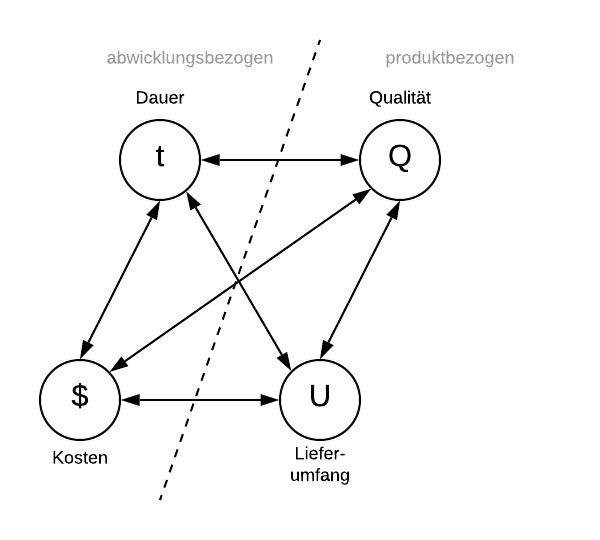
\includegraphics[height=5cm]{img/pm/teufelsquadrat.jpeg}
			\caption{Teufelsquadrat}
			\label{fig:pm_teufelsquadrat}
		\end{subfigure}
		\begin{subfigure}{.55\textwidth}
			\centering
			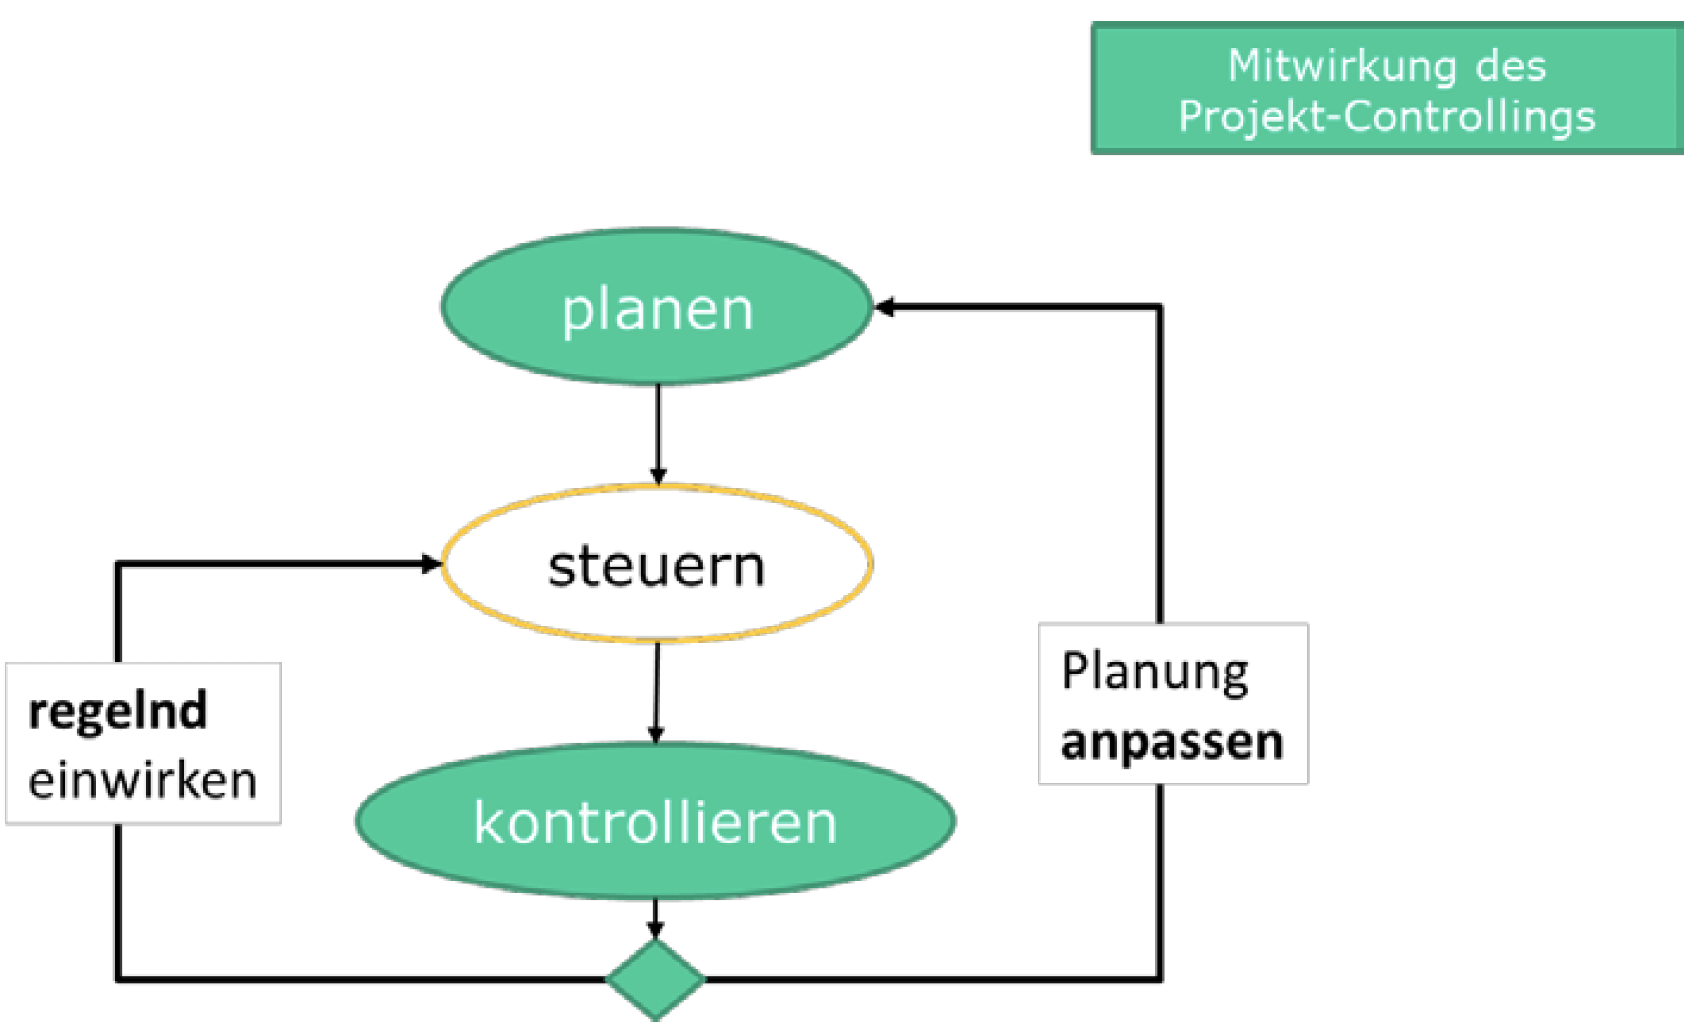
\includegraphics[height=6cm]{img/pm/steuerung.png}
			\caption{Steuerung vs. Regelung}
			\label{fig:pm_steuerung}
		\end{subfigure}
		\caption{Teufelsquadrat \& Steuerung vs. Regelung}
		\label{fig:pm_teufel_steuerung}
	\end{figure}

	\begin{itemize}
		\item Planungswerte durch Dimensionen des Teufelsquadrat repräsentiert
		\item Planungseinheit, die Einfluss nehmen kann, ist ein definiertes AP
		\item Die 4 Dimensionen sind voneinander abhängig,\\ 
		Änderung einer Dimension hat Reaktion auf anderer Achse zur Folge
	\end{itemize}

	\paragraph{Steuerung vs. Regelung}
	
	In einem Projekt wird geregelt, nicht nur gesteuert.
	(Wenn wir ein Fahrzeug "steuern", sind wir eig. regelnd unterwegs).
	
	\paragraph{Zusammenhang zw. Projektplanung \& Projektfortschritt überwachen}
	
	Aus Planung entsteht Basisplan zu Zeitpunkt $t_{0}$.
	Zu einem Zeitpunkt $t_{x}$ wird der Fortschritt des Projekts dann kontrolliert/überwacht.
	Je nachdem wie kritisch die Abweichungen sind werden Massnahmen ergriffen und ein neuer Plan zum Zeitpunkt $t_{x}$ erstellt (der wieder abgenommen werden muss).
	
	\begin{figure}[!htb]
		\centering
		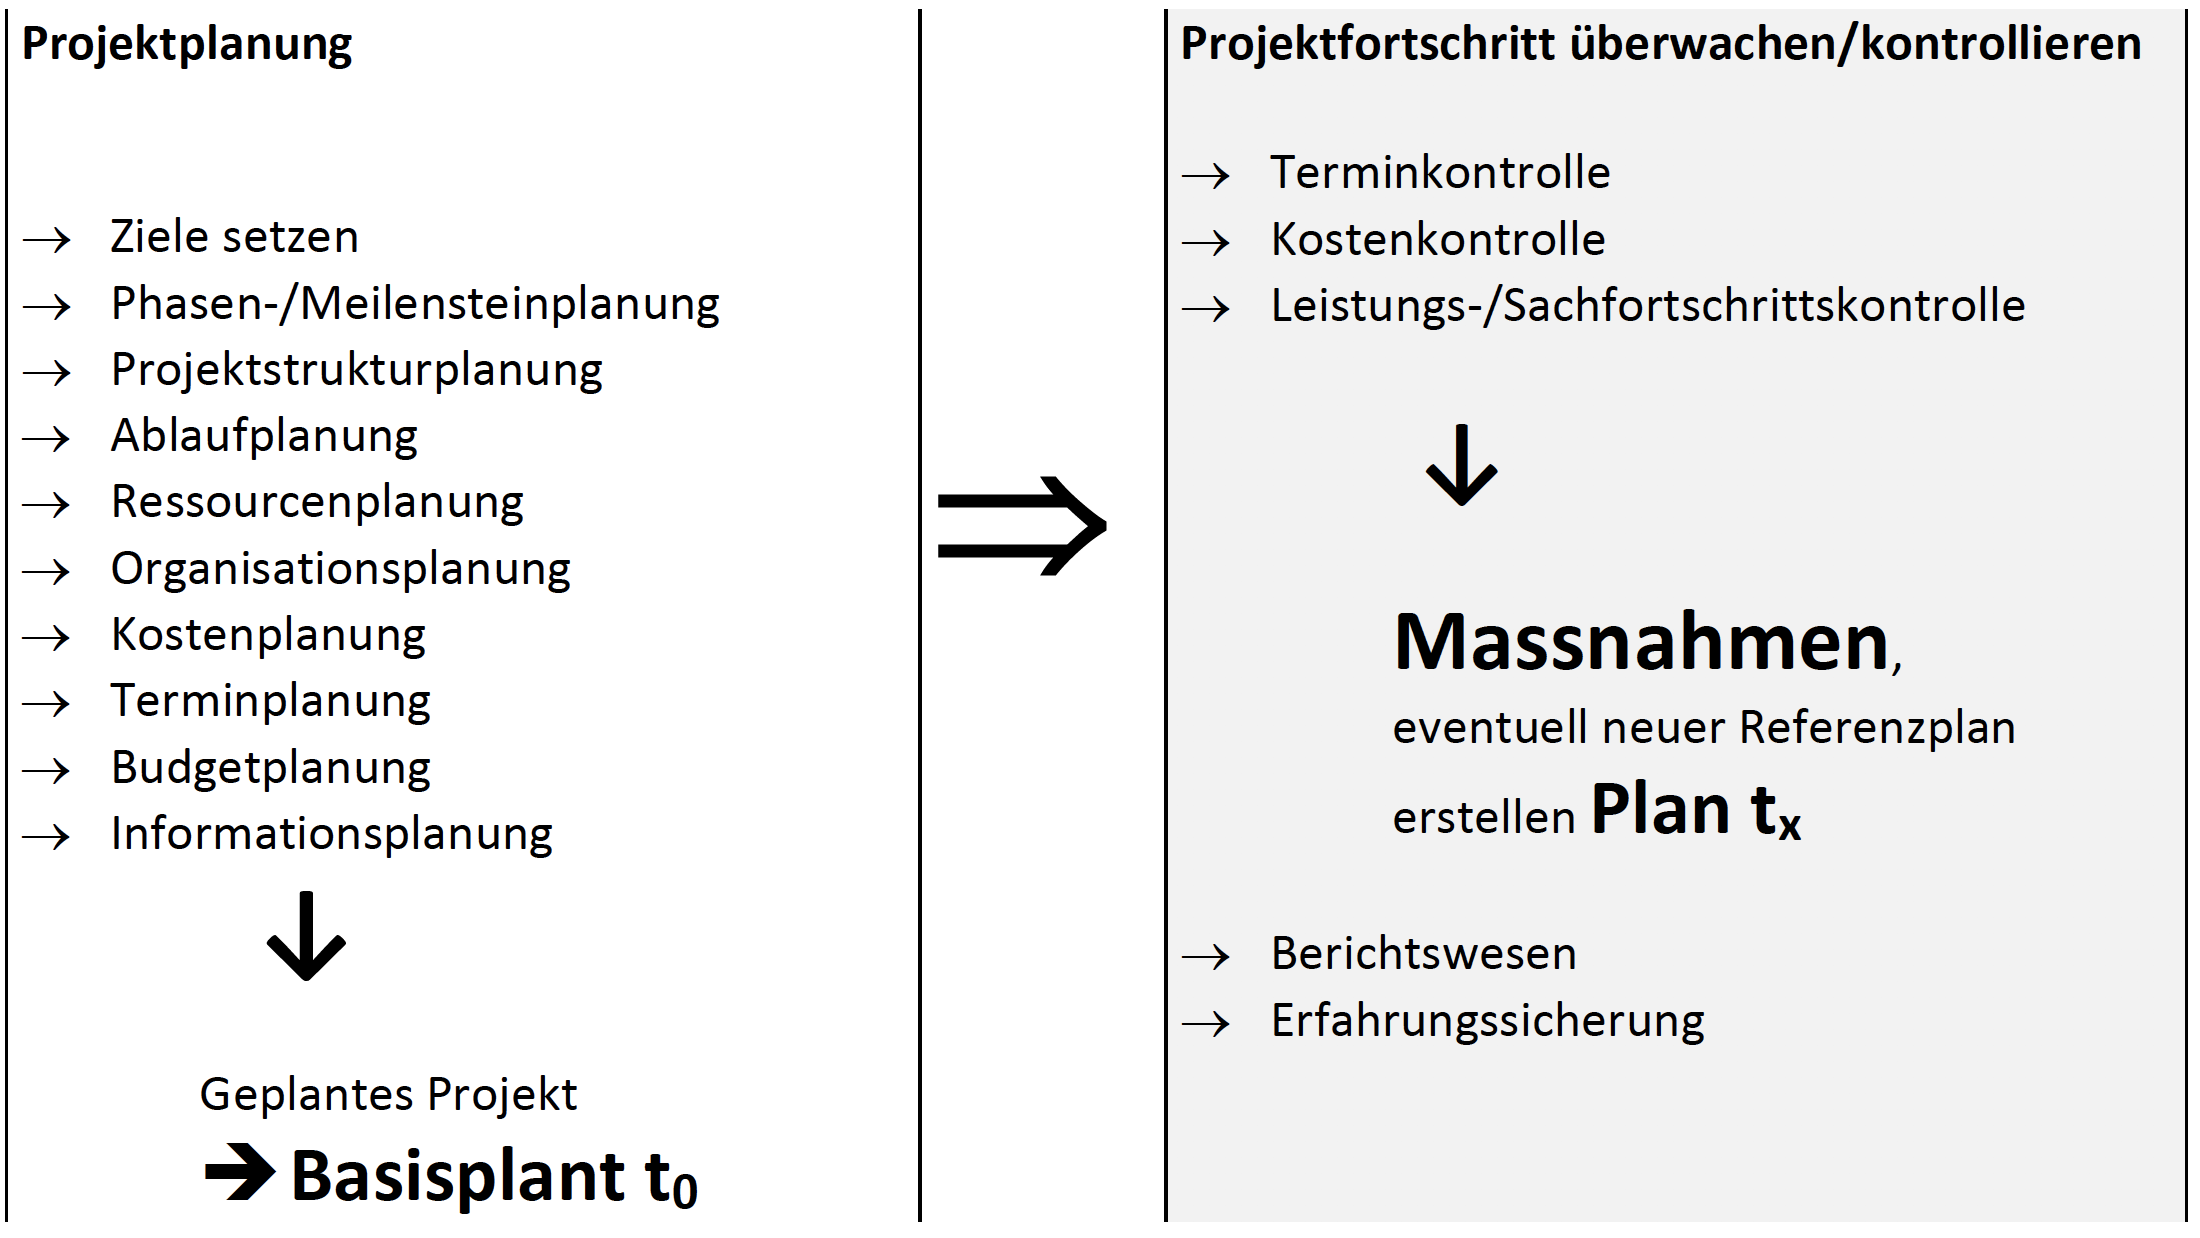
\includegraphics[height=6cm]{img/pm/basisplan.png}
		\caption{Zusammenhang Projektplanung / Projektfortschritt überwachen}
		\label{fig:pm_basisplan}
	\end{figure}

\newpage

		\subsection{Kontrollbereiche}
		
		\begin{itemize}
			\item \textbf{Definition "messen":}\\
			Kann als kontrollieren/überwachen interpretiert werden; 
			umfasst alle Aktivitäten, um projektbezogene Abweichungen zw. Plan- und Ist-Zustand aufzudecken
			\item Korrigierende Massnahmen sind Teil des Steuerns, nicht des Messens
			\item Unterscheiden:
				\begin{itemize}
					\item Planungskontrolle (Kontrolle bezieht sich auf Projektabwicklung)
					\item Realisierungskontrolle (Kontrolle auf das vom Projekt zu liefernde Produkt)
				\end{itemize}
		\end{itemize}
	
		\begin{figure}[!htb]
			\centering
			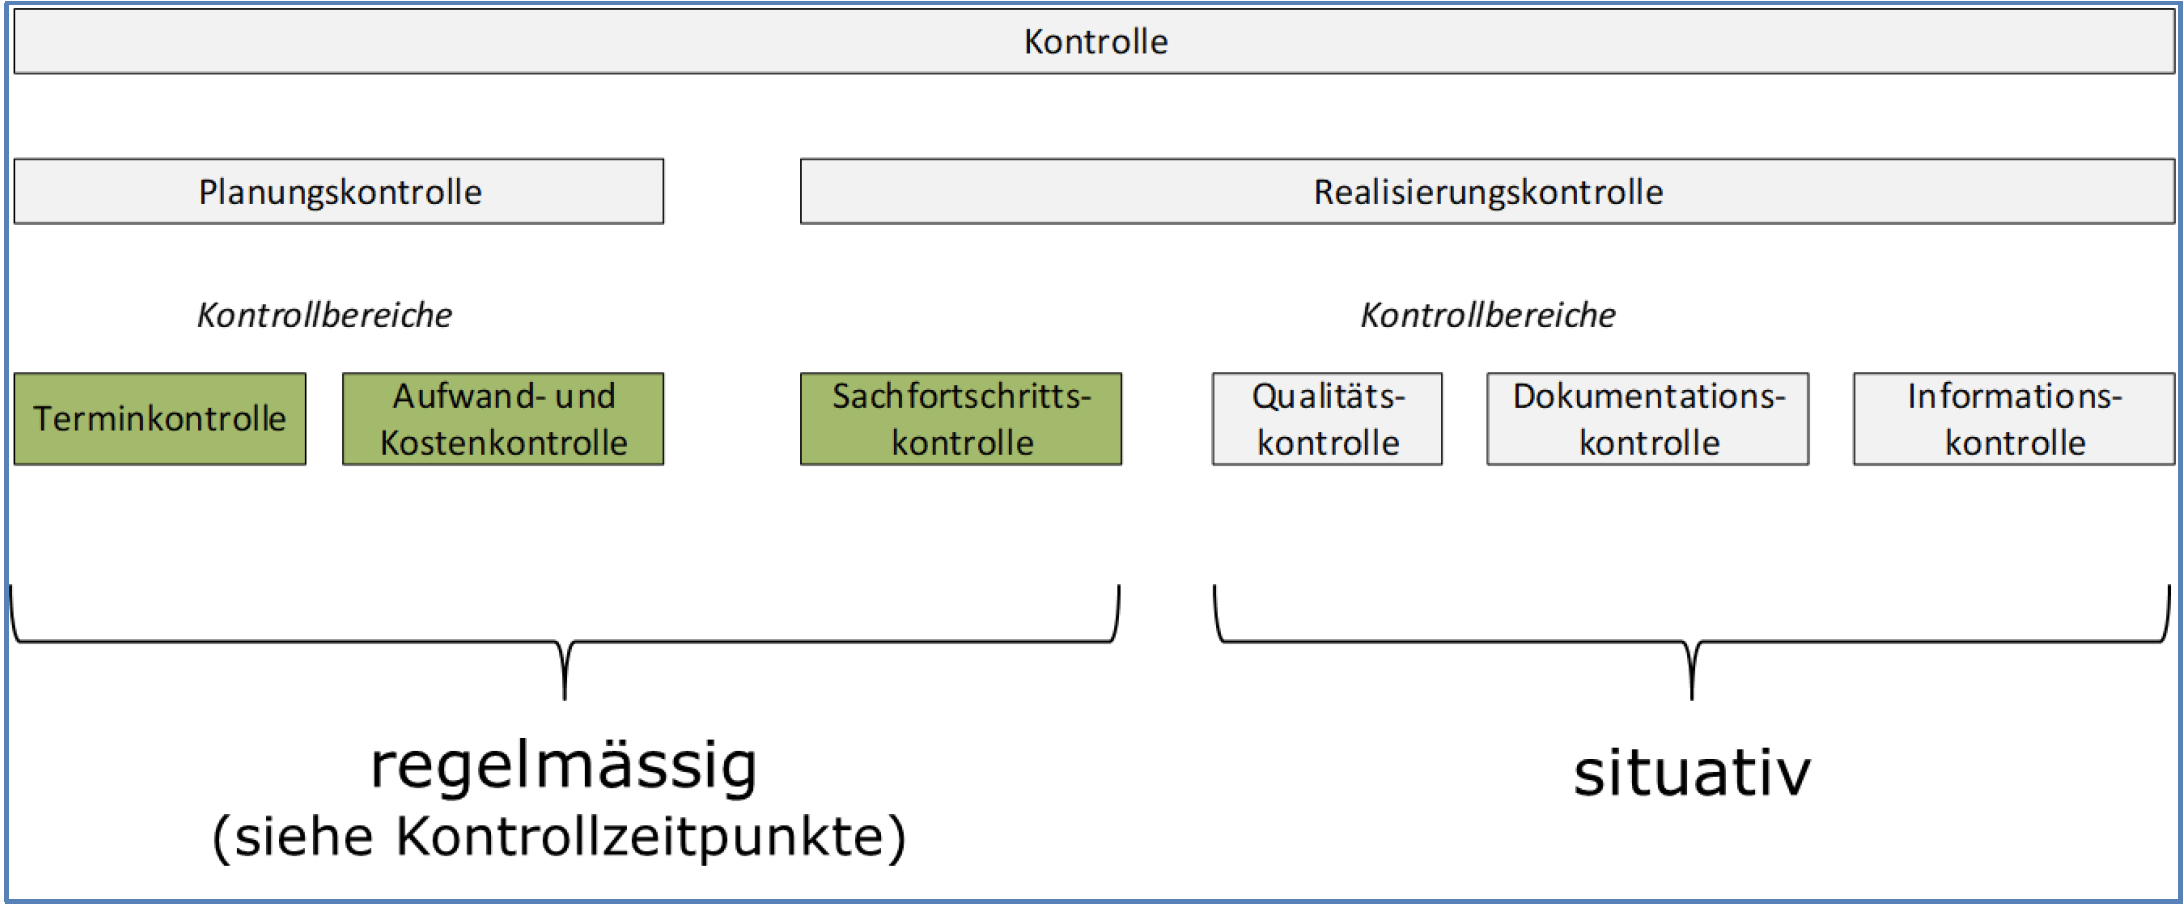
\includegraphics[height=5cm]{img/pm/kontrollbereiche.png}
			\caption{Kontrollbereiche in Projektabwicklung}
			\label{fig:pm_kontrollbereiche}
		\end{figure}
	
		\begin{itemize}
			\item \textbf{Terminkontrolle}
				\begin{description}
					\item[Ziel] Projektüberprüfung auf Einhaltung des geplanten Endtermins. Fokus auf kritische Pfade
					\item[Fragestellung] Sind in Planung vorgegebene Termine (Meilensteine) eingehalten worden?
					\item[Prognose] Wann wir das Projekt voraussichtlich beendet?
				\end{description}
			\item \textbf{Kostenkontrolle}
				\begin{description}
					\item[Ziel] Überprüfung des Projekts aus Einhaltung geplanter Kosten
					\item[Fragestellung] Sind bis zum Kontrollzeitpunkt kumulierte Kosten eingehalten worden?
					\item[Prognose] Zu welchen Kosten wird Projekt voraussichtlich abgeschlossen?
				\end{description}
			\item \textbf{Leistungs-/Sachfortschrittskontrolle}
				\begin{description}
					\item[Ziel] Produckt pberprüfen auf Erreichung des geplanten Lieferumfangs
					\item[Fragestellung] Wie weit ist Arbeit am Produkt fortgeschritten?
					\item[Prognose] Wird Projektgegenstand wie abgemacht geliefert?
				\end{description}
		\end{itemize}
	
		\paragraph{Kontrollzeitpunkte}
	
		\begin{itemize}
			\item Festlegen der Kontrollzeitpunkte nach:
				\begin{itemize}
					\item \textbf{nach einer Zeitdauer oder Arbeitsvolumen}\\
						nach vorgegebener Zeitdauer oder bei Erreichen eines Kontrollvolumens, egal ob bei Phasenende oder Resultat.
						Zeitdauer typischerweise zw. 1-3 Monaten, Volumen bei 100-200 geleisteten Personentagen.
					\item \textbf{bei Erreichung eines Resultates}\\
						Lieferobjekt nach Erstellung möglichst unmittelbar kontrollieren, um allfällige Fehler schnell erkennen zu können
					\item \textbf{bei Erreichung von Phasenende/Meilenstein}\\
						Phasenabschluss ist prädestiniert für einen Kontrollzeitpunkt
				\end{itemize}
		\end{itemize}
		
\newpage

	\subsection{Terminkontrolle}
		
	\begin{itemize}
		\item \textbf{Wieso Projekttermine kontrollieren?}\\
			Endzeitpunkt des Projekts sicherstellen, erreichte Projekttermine müssen gesichert werden
		\item Termine haben mit Dauer eines Projekts zu tun, nur kontrollierbar wenn sie eindeutig benannt sind
		\item Typische Termine:
			\begin{itemize}
				\item Meilensteintermine
				\item Start- und Endtermine von APs
				\item Audit- \& Reviewtermine
				\item Projektanfangs- und -endtermin
				\item Weitere wie Berichtstermine etc.
			\end{itemize}
		\item Dauer aus Aufwand und verfügbaren Ressourcen:\\
			\\
			$Dauer[Tage] = \frac{Aufwand[PT]}{Personen[P]}$
	\end{itemize}
		
		\subsubsection{Termintreue (\%)}
		
		Kennzahl, wie viele vergangene Termine eingehalten werden konnten oder eben nicht.
		Diese Kennzahl gibt Auskunft über Termintreue bzw. lässt aufschliessen, wie akkurat die Planung war (Aufwand \& Dauer)
		
		\begin{quote}
			Termintreue [\%] = $\frac{\#TermineEingehalten}{\#Termine} \times 100[\%]$
		\end{quote}
	
		\subsubsection{Zeitlicher Fortschrittsgrad (\%)}
		
		\begin{quote}
			Zeitl. Fortschrittsgrad$_{IST}$ [\%] = $\frac{Dauer[Wochen]}{prog.Gesamtdauer[Wochen]} \times 100\%$\\
			\\
			Freiheitsgrad PLAN: zeitFG$_{PLAN}$ = $\frac{Istdauer}{geplante Dauer}$\\
			\\
			Freiheitsgrad IST: zeitFG$_{IST}$ = $\frac{Istdauer}{voraussichtliche Dauer}$\\
			\\
			\textit{(Abweichung zw. zeitFG$_{PLAN}$ \& zeitFG$_{IST}$: grobes Indiz für Einhaltung des Endtermins)}
		\end{quote}
		
		\subsubsection{Termin-Trenddiagramm}
		
		\begin{minipage}{.45\textwidth}
			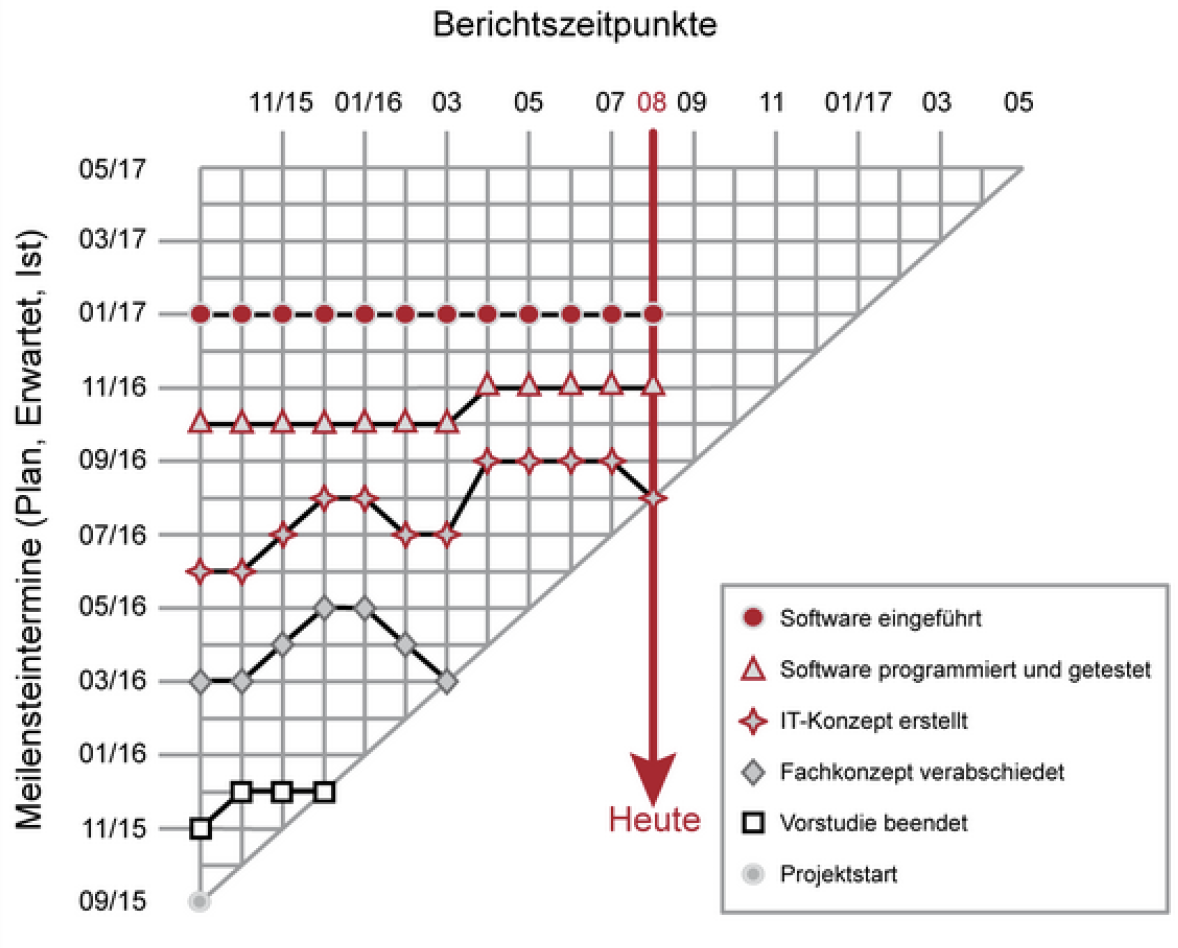
\includegraphics[height=5cm]{img/pm/termintrend.png}
		\end{minipage}
		\begin{minipage}{.45\textwidth}
			\textbf{Leselogik:}
			\begin{itemize}
				\item Kurve nach oben, wenn Termine immer wieder nach hinter verschoben.
				Strebt weg von ursprünglich geplantem Termin (weg von der Diagonale)
				\item Kurvenverlauf horizontal, wenn keine Terminabweichungen erkennbar sind
				\item Kurve nach unten, wenn Termine vorverschoben werden können (strebt der Diagonale entgegen)
			\end{itemize}
		\end{minipage}
		\vspace{1em}
		\begin{itemize}
			\item \textbf{Vorteile:} einfach, schnell zu erstellen, Terminabweichungen sofort erkennbar, geeignetes Kommunikationsmittel (innerhalb/ausserhalb Projekt), Abstimmungsdefizite erkennbar, fördert Terminbewusstsein
			\item \textbf{Nachteile:} subjektive Einschätzung, Trendkurve allein nicht ausreichen zur Ursachenanalyse, Diagramm muss kommentiert sein
		\end{itemize}
		
\newpage

	\subsection{Kostenkontrolle (Aufwandkontrolle)}
	
			\paragraph{Wieso Projektkosten kontrollieren?}
			
			Ziel der Kostenkontrolle ist, vereinbarten Kostenrahmen des Projekts sicherzustellen.
			Der gemäss Planung vorgesehene zeitliche Kostenanfall muss gesichert werden.
			Kosten können \textit{time} oder \textit{material} sein.
			
		\subsubsection{Ist- und Plankosten}
		
		\begin{itemize}
			\item In der Kostenkontrolle werden zwei Kosten einander gegenübergestellt \& verglichen:
				\begin{itemize}
					\item IST-Kosten (zum Kontrollzeitpunkt $t_x$ aufgelaufene effektive Kosten, kumuliert)
					\item Plankosten (zum Zeitpunkt nach Planung verbrauchte Kosten, kumuliert)
				\end{itemize}
			\item Es können 3 mögliche Zustände vorliegen (siehe Abbildung \ref{fig:pm_kostenkurve}):
				\begin{itemize}
					\item IST-Kosten liegen zum Zeitpunkt $t_x$ unter dem geplanten Verbrauch
					\item IST-Kosten entsprechen zum Zeitpunkt $t_x$ dem geplanten Verbrauch
					\item IST-Kosten liegen zum Zeitpunkt $t_x$ über geplantem Verbrauch
				\end{itemize}
			\item Es interessieren primär Personalkosten (reflektieren effektiv geleistete Aufwände)
		\end{itemize}
	
		\begin{figure}[!htb]
			\centering
			\begin{subfigure}{.45\textwidth}
				\centering
				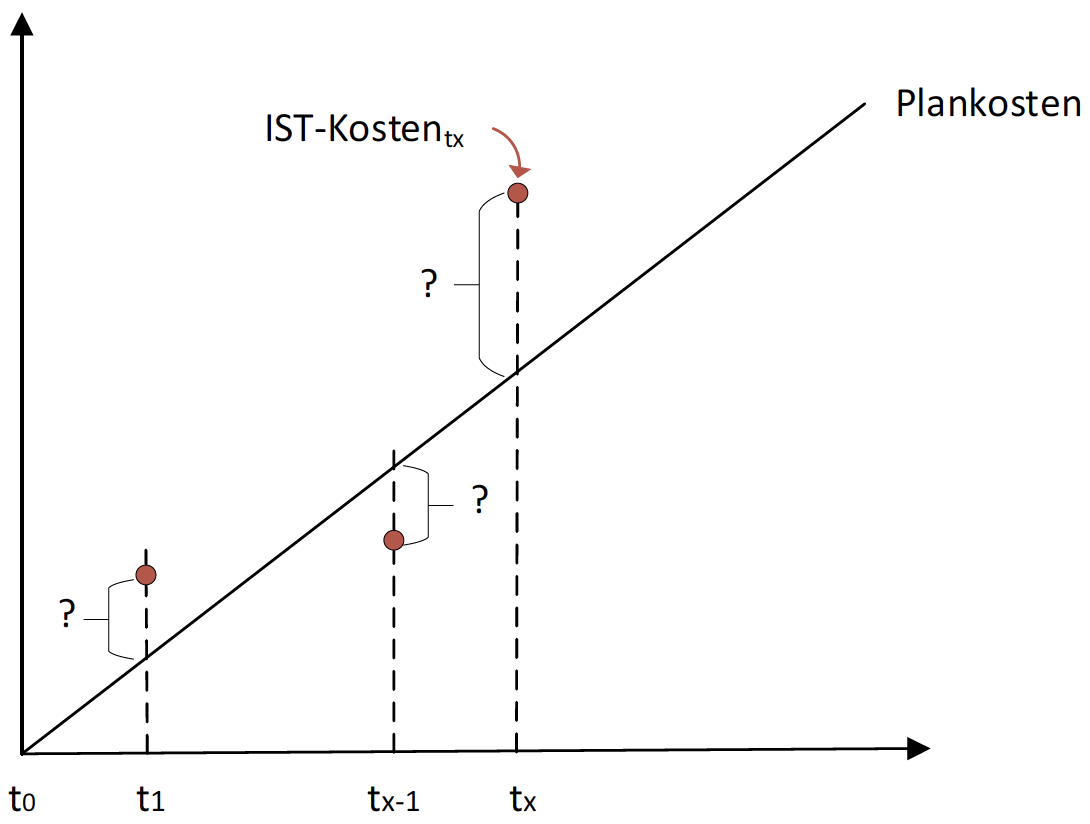
\includegraphics[height=4cm]{img/pm/kostenkurve.png}
				\caption{schematische Kostenkurve}
				\label{fig:pm_kostenkurve}
			\end{subfigure}
			\begin{subfigure}{.45\textwidth}
				\centering
				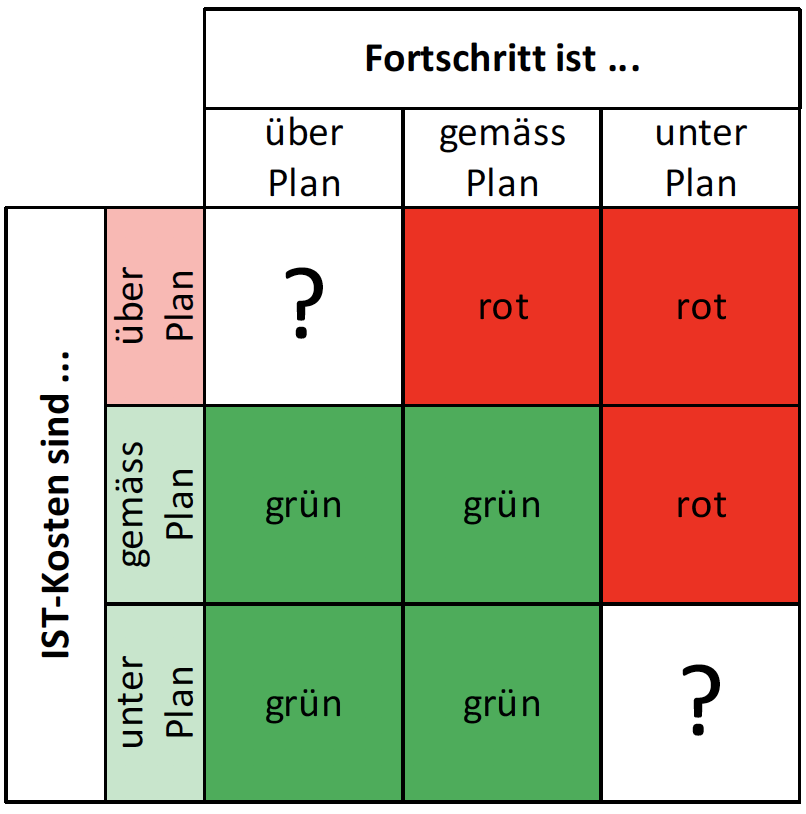
\includegraphics[height=4cm]{img/pm/kostenbewertung.png}
				\caption{Bewertungsbereich von Kosten}
				\label{fig:pm_kostenbewertung}
			\end{subfigure}
		\end{figure}
	
		\begin{itemize}
			\item Zum Zeitpunkt $t_x$ mehr Ressourcen verbraucht als geplant\\
			Zum Zeitpunkt $t_{x-1}$ jedoch weniger als geplant
			\item Zustand bei $t_x$ so interpretierbar, dass Projekt weiter fortgeschritten als geplan, da offenbar mehr Aufwände rapportiert als geplant
			\item Oder dass trotz Mehrkosten resultatmässig weniger erreicht wurde als bei $t_x$ geplant
			\item Kostenkontrolle muss deshalb unbedingt den \textbf{Sachfortschritt} des Projekts miteinbeziehen
		\end{itemize}
	
		\subsubsection{SOLL-Kosten (Earned Value)}
		
		Aufgelaufene IST-Kosten zum Kontrollzeitpunkt $t_x$ reflektieren geleisteten (Personen-)Aufwand im Projekt.
		Ist aber nicht gleichbedeutend mit Fortschritt bezogen auf das zu erstellende Endresultat (Produkt).
		Von Interesse ist, was mit rapportiertem Aufwand geleistet wurde!
		Kostenkontrolle muss immer auch den Leistungsstand in Betrachtung ziehen.\\
		\textbf{Arbeitswert, SOLL-Kosten:} Entspricht Kosten, die in einem AP bei einem bestimmten Fortschrittsgrad (FG) nach Plan hätten anfallen dürfen. 
		Earned Value kann maximal den Planwert (Planned Value PV) des APs erreichen.
			
			\paragraph{Beispiel}
			
			\begin{itemize}
				\item Arbeitspaket:
				\begin{description}
					\item[Plankosten] CHF 10'000
					\item[IST-Kosten] CHF 7'500
					\item[Fortschrittsgrad] 25\%
				\end{description}
				\item AP wird in der Hälfte seiner Dauer überprüft, zum Zeitpunkt t$t_x$ sind IST-Kosten CHF 7'500
				\item FG ist aber nur bei 25\% (nicht wie erwartet bei 50\%, bei Hälfte der Dauer)
				\item Es hätten nur $\frac{1}{4}$ der Plankosten (also CHF 2'500) anfallen dürfen
				\item \textbf{SOLL-Kosten} liegen somit bei CHF 2'500
			\end{itemize}
		
\newpage

	\subsection{Leistungskontrolle / Sachfortschrittskontrolle}
	
	\begin{itemize}
		\item \textbf{Wieso Leistungsfortschritt kontrollieren?}\\
			Soll den Lieferumfang des Projekts sicherstellen.
		\item Dazu müssen zum Zeitpunkt $t_x$ vorgesehene Leistungen, Resultate \& Fortschritt gesichert werden
	\end{itemize}

		\subsubsection{Methoden zur Bestimmung des Fortschrittsgrads}
		
		Zur Berechnung des Arbeitswertes (SOLL-Kosten) muss Fortschrittsgrad zum Kontrollzeitpunkt $t_x$ bestimmt sein.
		Dazu bieten sich folgende Möglichkeiten an:
		\vspace{1em}
		\begin{itemize}
			\item \textbf{Meilensteinmethode}\\ 
				Anzahl erreichte Meilensteine vs. Total aller Meilensteine
			\item \textbf{Relativer Fertigstellungsgrad / Befragung}\\
				relative Betrachtung der Fertigstellung;
				Ermittlung einer genauen \%-Grösse, sehr subjektiv
			\item \textbf{0/50/100\%-Methode}\\
				Betrachtung, welche noch nicht gestartetes AP mit 0\%, begonnenes AP mit 50\% und abgeschlossenes AP mit 100\% bewertet
			\item 0/100\%-Methode\\
				Betrachtung, welche erst bei Abschluss eines AP 100\% vergibt, alle laufenden / nicht begonnenen APs werden mit 0\% bewertet
			\item \textbf{Restaufwandschätzung}\\ 
				zukunftsorientierte Methode;
				Statt erbrachte Leistung zu bewerten wird Restaufwand geschätzt (wieviel Aufwand muss noch geleistet werden), Substraktion des Restaufwands von geplantem Aufwand ergibt eine Abschätzung des Fortschritts (unter Berücksichtigung eingesetzter Ressourcen)
		\end{itemize}
		
		\begin{figure}[!htb]
			\centering
			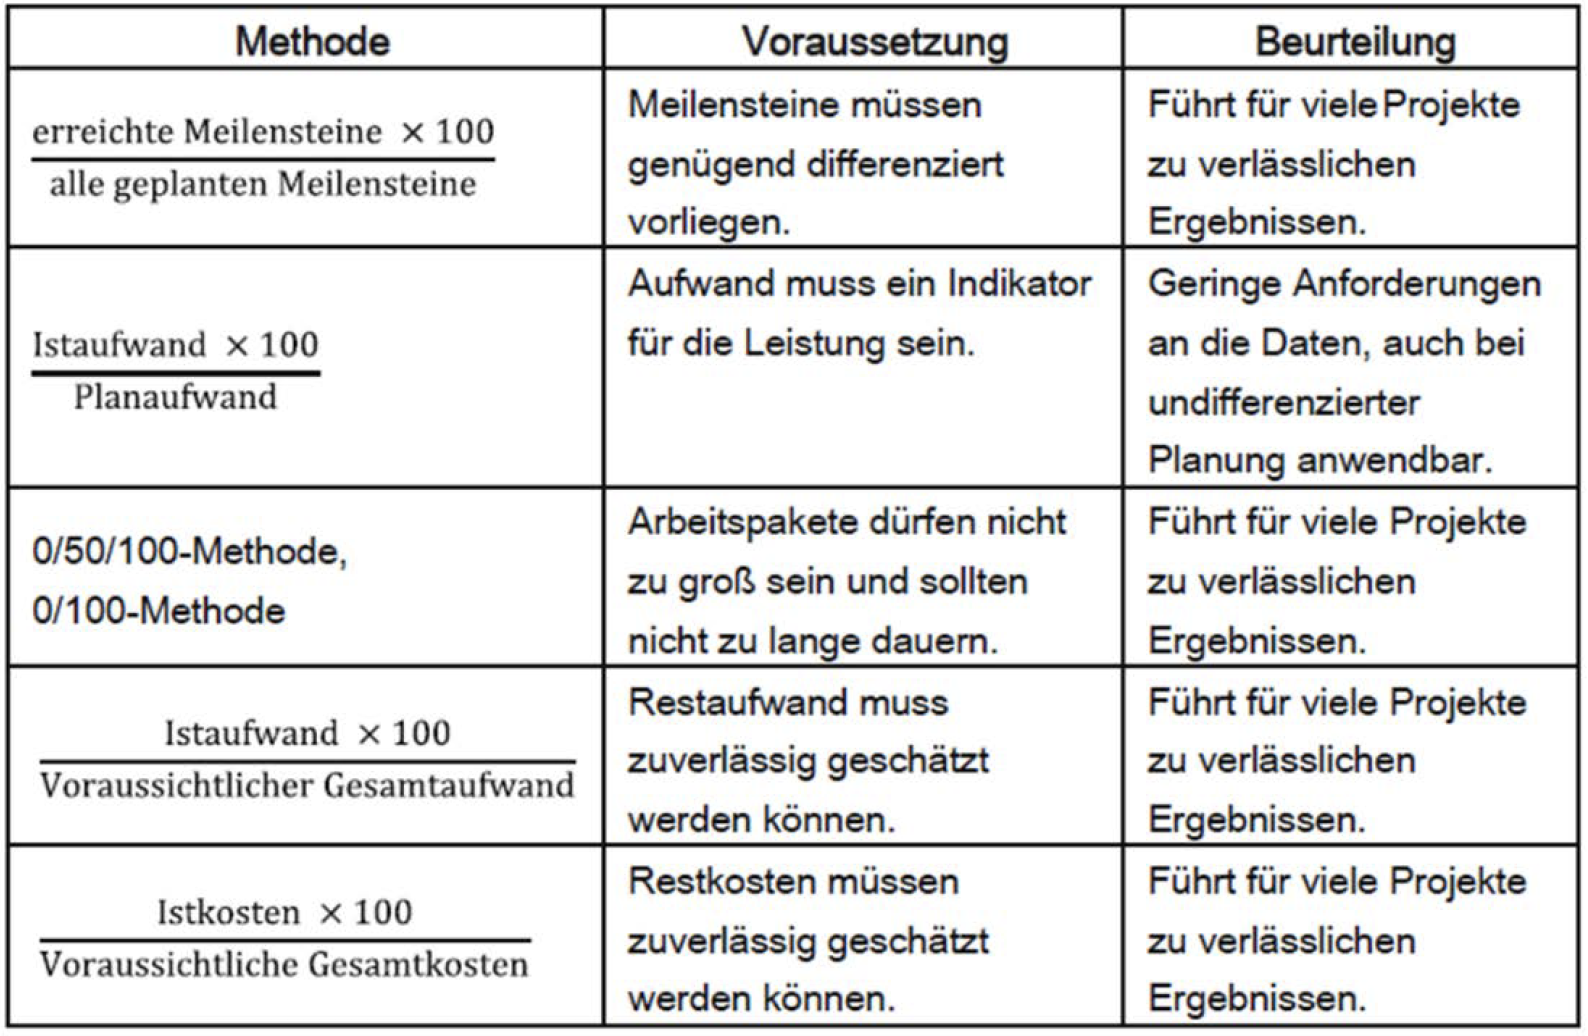
\includegraphics[height=8cm]{img/pm/fg_methoden.png}
			\caption{Möglichkeiten zur Bestimmung des Fortschrittsgrads}
			\label{fig:pm_fg_methoden}
		\end{figure}
	
\newpage
		
		\paragraph{Beispiel}
		
		Gegeben ist ein Arbeitsplan mit APs A bis F.
		Für jedes ist effektiver Leistungsfortschritt indiziert (100\% oder 25\%).
		Auch PLAN- und IST-Kosten sind für das Projekt bekannt:
		
		\begin{figure}[!htb]
			\centering
			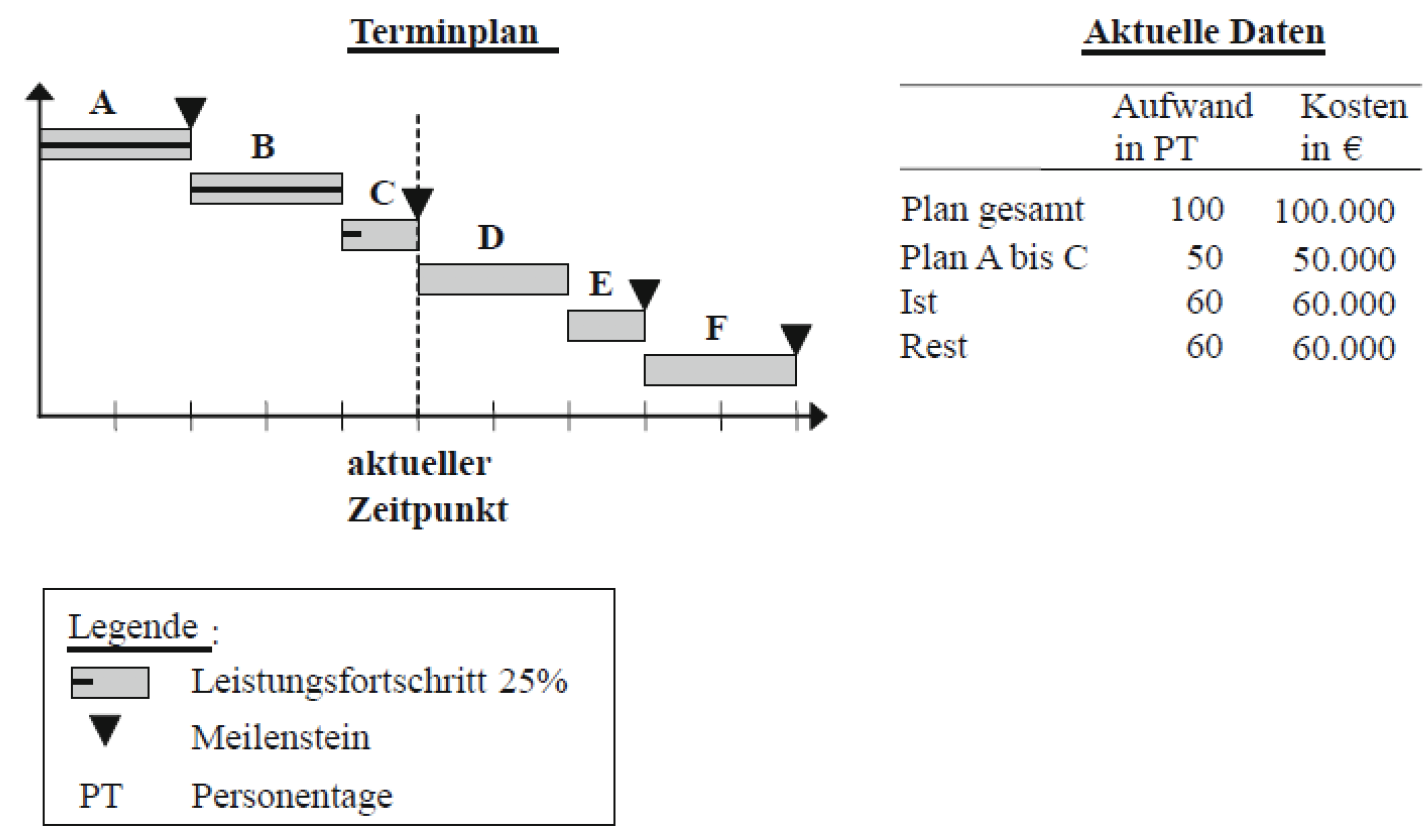
\includegraphics[height=6cm]{img/pm/leistung_01.png}
			\caption{Terminplan mit aktuellen Daten}
			\label{fig:pm_leistung_01}
		\end{figure}
		\noindent
		Die Arbeitswerte (erwirtschafteter Wert) für die APs lässt sich nach 0/50/100-Methode folglich berechnen:
		
		\begin{figure}[!htb]
			\centering
			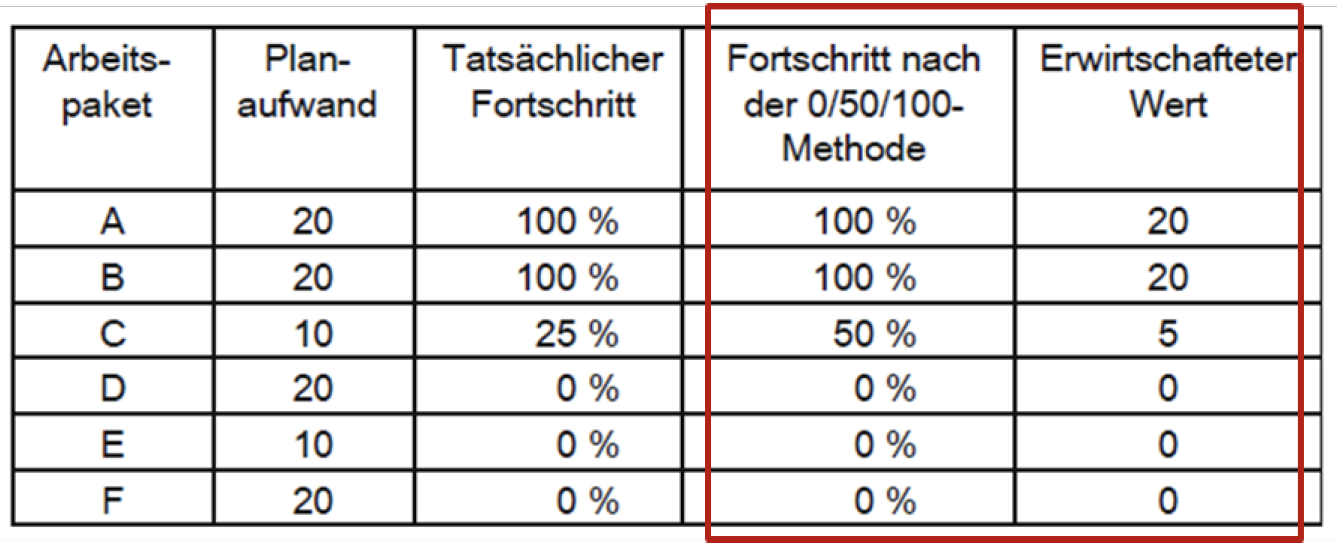
\includegraphics[height=4cm]{img/pm/leistung_02.png}
			\caption{Berechnung des Fortschritts \& erwirtschaftetem Wert}
			\label{fig:pm_leistung_02}
		\end{figure}
		
	\subsection{Integrierte Kontrollsicht - Leistung-/Kosten-Kontrolle}
	
	Kosten reflektieren geleisteten Personenaufwand, ist jedoch nicht gleichbedeutend mit Fortschritt bezogen auf das zu erstellende Endresultat (Produkt).
	Kostenkontrolle muss auch Leistungsstand (Fortschritt) mit einbeziehen.\\
	$\rightarrow$ Earned-Value-Methode
	
		\subsubsection{Earned Value (EV)}
		
		\begin{itemize}
			\item Neben PLAN- und IST-Kosten auch SOLL-Kosten (Earned Value) betrachten
			\item Synonym: \textit{Budgeted Cost of Work Performed - BCWP}
			\item \textbf{EV} entspricht denjenigen \textbf{Kosten, die für Erreichung des eruierten FG hätten anfallen dürfen}
			\item EV eines AP zum Kontrollzeitpunkt $t_x$ berechnen:\\
			\\
			EV$_{tx}$ = FG$_{tx} \times$ Plankosten$_{AP}$\\
			\textit{(EV eines AP kann nie höher sein als die Plankosten eines AP)}
		\end{itemize}
	
\newpage

		\subsubsection{Earned Value Methode (EVM)}
		
		\begin{figure}[!htb]
			\centering
			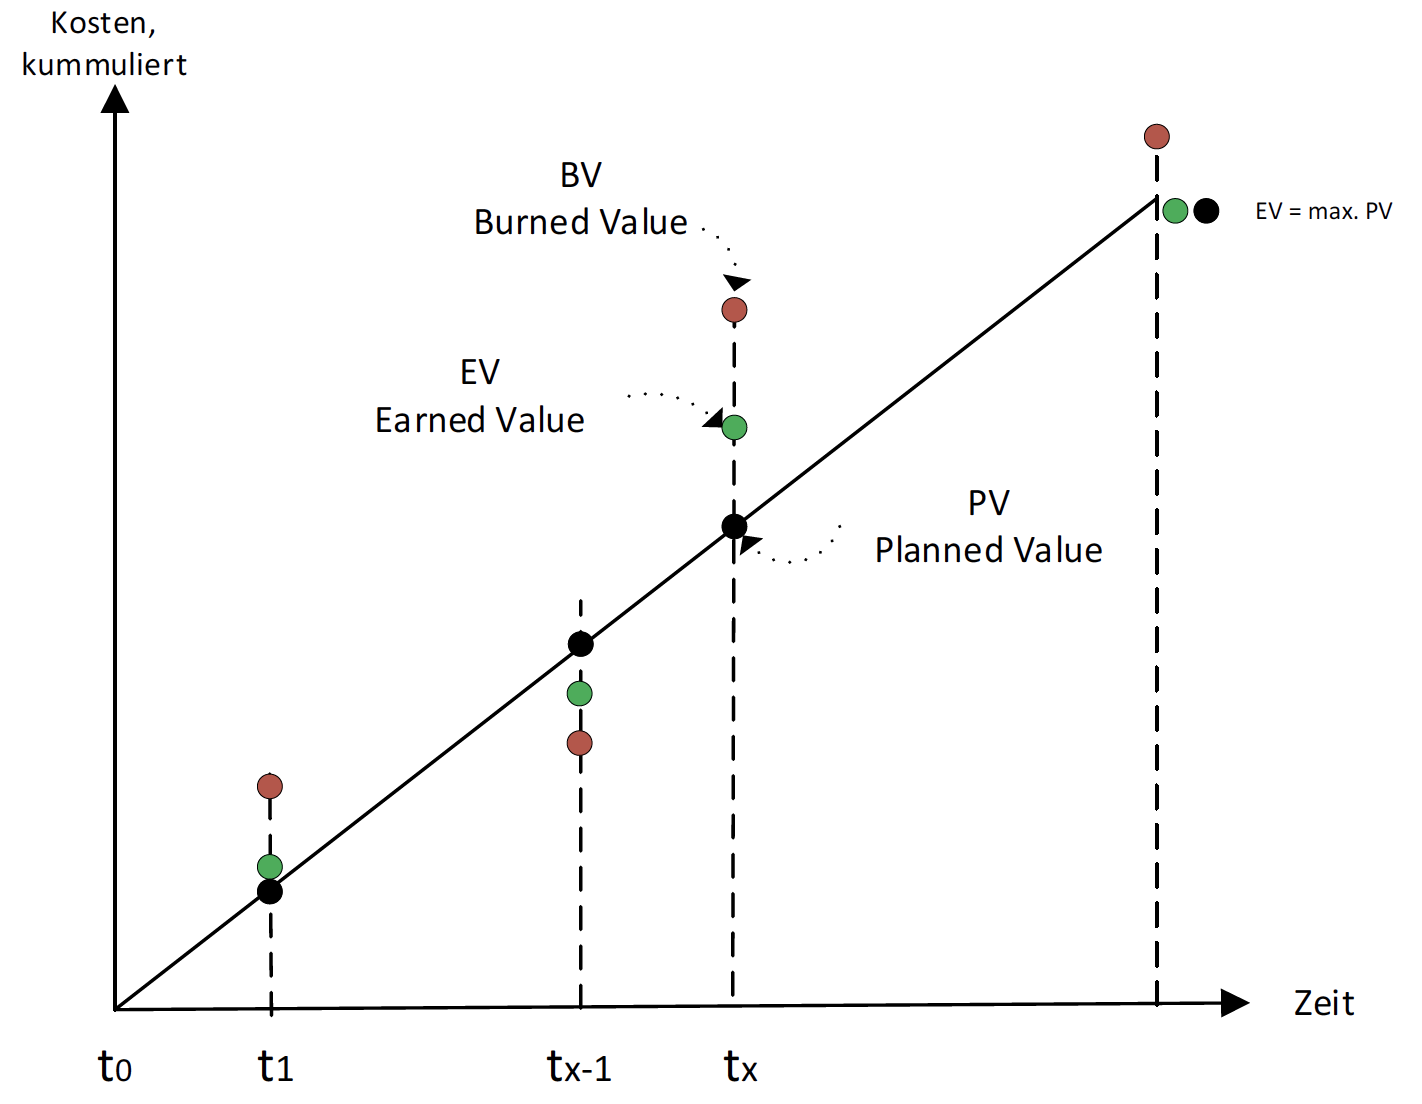
\includegraphics[height=5cm]{img/pm/evm_dia.png}
			\caption{PV, BV und EV auf der Zeitachse}
			\label{fig:pm_evm_dia}
		\end{figure}
		
		\textbf{Kennzahlen:}
		\begin{itemize}[itemsep=0.5em]
			\item \textbf{Burned Value (BV)}\\
			Kumulierte IST-Kosten (auch \textit{Actual Cost (AC)} oder \textit{Actual Cost of Work Performed (ACWP)})\\
			Herkunft: aus der Rapportierung
			
			\item \textbf{Planned Value (PV)}\\
			Kumulierte PLAN-Kosten (auch \textit{Budgeted Cost of Work Scheduled (BCWS)})\\
			Herkunft: aus der Planung
			
			\item \textbf{Earned Value (EV)}\\
			Wie erläutert (auch \textit{Budgeted Cost of Work Performed (BCWP)})\\
			Herkunft: berechnet aus eruiertem Fortschrittsgrad (\%) bei $t_x$ mal Plankosten des AP
			
			\item \textbf{Scheduled Performance Index (SPI)}\\
			Zeitliche Kenngrösse, sagt aus ob Projekt vor oder hinter dem Plan liegt\\
			Berechnung: $SPI = \frac{EV}{PV}$
				\begin{description}
					\item[SPI = 1] Projekt ist planmässig unterwegs
					\item[SPI > 1] Erbrachte Leistung grösser als geplant, Projekt schneller als geplant
					\item[SPI < 1] Erbrachte Leistung kleiner als geplant, Projekt langamer als geplant\\
				\end{description}
			\begin{itemize}
				\item Terminprognose mit SPI: $progDauer = \frac{Dauer.geplant}{SPI}$\\
			\end{itemize}
			
			\item \textbf{Cost Performance Index (CPI)}\\
			Kostenbezogene Kenngrösse, sagt aus ob Projekt über oder unter Plan läuft\\
			Berechnung: $CPI = \frac{EV}{BV}$
				\begin{description}
					\item[CPI = 1] Projekt kostenmässig gemäss Plan unterwegs
					\item[CPI > 1] Erbrachte Leistung grösser als tatsächliche Kosten, Projekt kostengünstiger als geplant
					\item[CPI < 1] Erbreachte Leistung kleiner als tatsächliche Kosten, Projekt teurer als geplant\\
				\end{description}
			\begin{itemize}
				\item Kostenprognose mit CPI: $progKosten = \frac{Kosten.geplant}{CPI}$\\
			\end{itemize}
			
		\end{itemize}
		
\newpage

		\subsubsection{Beispiel einer Anwendung der EVM}
		
		\begin{figure}[!htb]
			\centering
			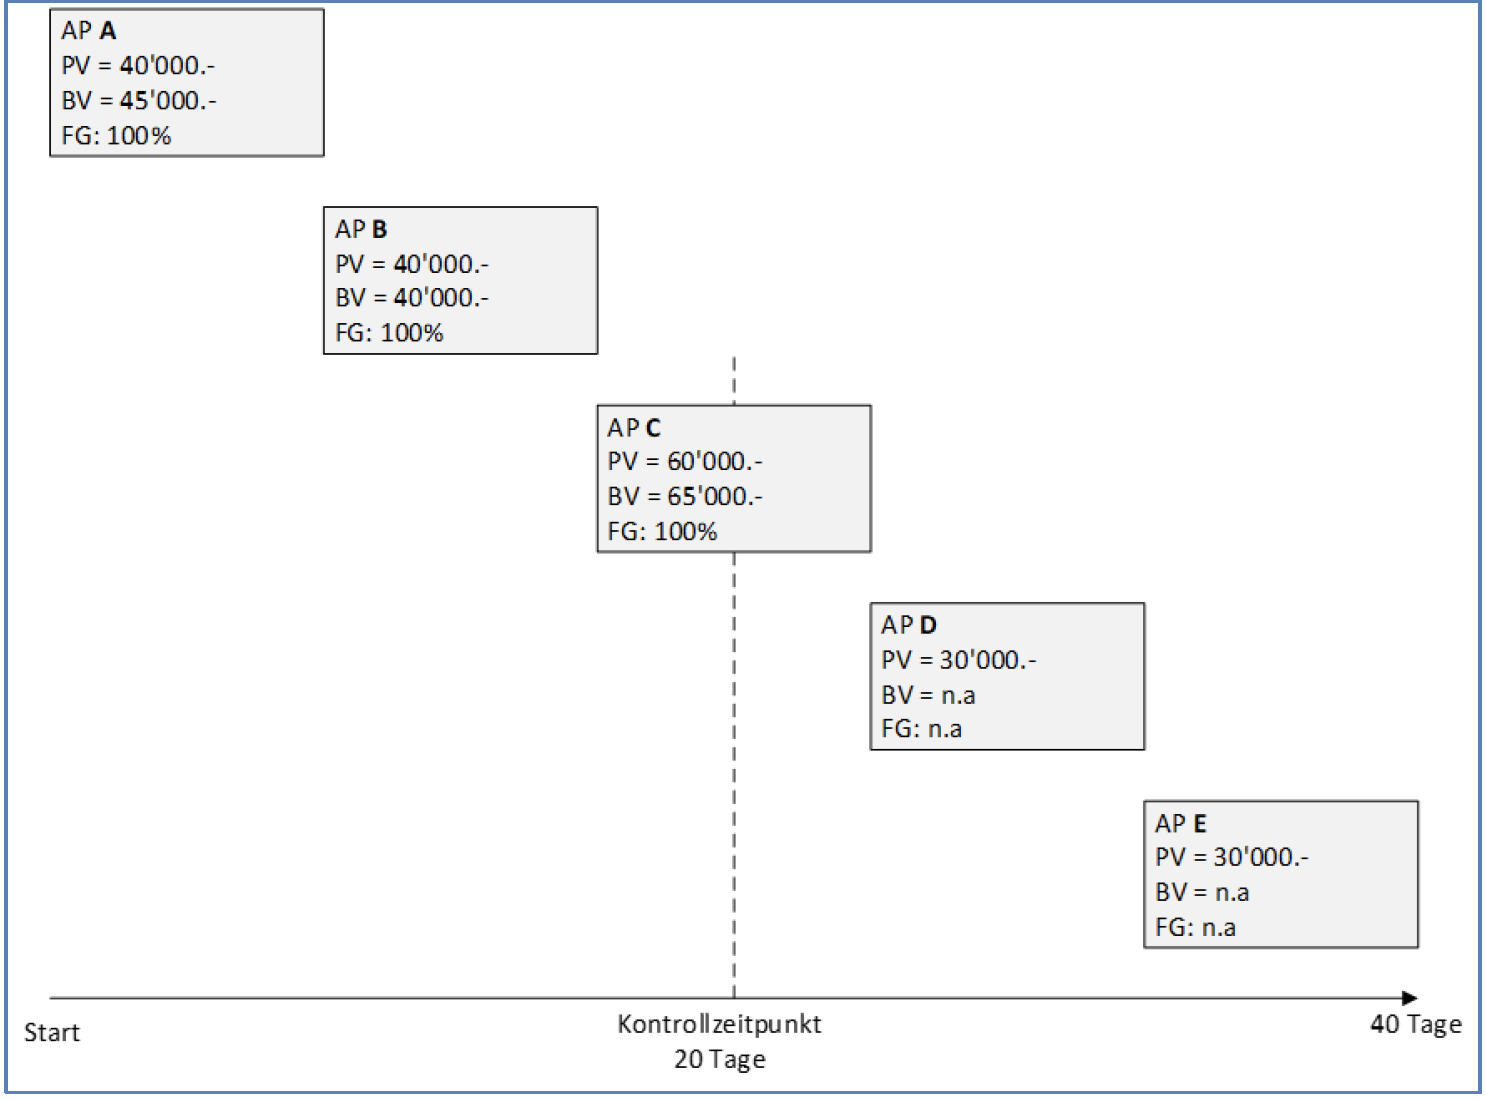
\includegraphics[height=7cm]{img/pm/evm_example.png}
			\caption{Übersicht von AP mit jeweiligen Werten}
			\label{fig:pm_evm_example}
		\end{figure}
	
		\begin{itemize}[itemsep=.5em]
			\item \textbf{PV} bei $t_x$: 40'000 + 40'000 + $\frac{60'000}{2}$ = 110'000 CHF
			\item \textbf{BV} bei $t_x$: 45'000 + 40'000 + 65'000 = 150'000 CHF
			\item \textbf{EV} bei $t_x$: 100\% $\cdot$ 40'000 + 100\% $\cdot$ 40'000 + 100\% $\cdot$ 60'000 = 140'000 CHF\\
				\textit{(EV berechnet sich auf Plankosten des gesamten AP)}
			\item \textbf{SPI}: $\frac{EV}{PV} = \frac{140'000}{110'000} = 1.3$\\
			prog. Endtermin: $\frac{Dauer.geplant}{SPI} = \frac{40}{1.3} =$ 31 Tage
			\item \textbf{CPI}: $\frac{EV}{BV} = \frac{140'000}{150'000} = 0.9$\\
			prog. Kosten: $\frac{Kosten.geplant}{CPI} = \frac{200'000}{0.9} = $215'000 CHF
		\end{itemize}
	
		\subsubsection{Erfahrungssicherung}
		
		\begin{itemize}
			\item Aufgetretene Probleme werden nach \textit{vermeidbar}, \textit{kaum vermeidbar} und \textit{nicht vermeidbar} aufgeteilt
			\item Fragen, die zu beantworten sind:
				\begin{itemize}
					\item Erfahrungen in Zusammenarbeit mit Lieferanten, Kunden, Fachabteilungen etc.?
					\item Qualität der Teamarbeit?
					\item Zweckmässigkeit des gewählten Vorgehen im Projekt?
					\item Bewährten sich die eingesetzten Instrumente?
					\item Angemessene Arbeitspakete (Aufwand, Dauer)?
					\item Kompetenzen \& Verantwortung richtig zugeteilt?
				\end{itemize}
		\end{itemize}
			
		\subsubsection{Reporting / Berichtswesen}
		
		Berichtswesen und Projektdokumentation obliegen der Fortschrittskontrolle.
		Ein akkurates Berichtswesen muss folgende 3 Kriterien erfüllen:
			\begin{itemize}
				\item Aktualität
				\item Empfängerbezogenheit
				\item Entscheidungsorientierung
			\end{itemize}
	
\newpage

	\subsection{Projekt steuern}
	
		\subsubsection{"Adding People to a late project makes it even later"}
		
		Was, wenn Projekt in Schieflage gerät?
		Massnahmen gefragt, welche sind jedoch wirksam?\\
		\textbf{Wieso?} Möglich ist, dass Kommunikations- bzw. Abstimmungsaufwand entlang Teamgrösse wächst.
		Je mehr Mitglieder einem Team zugehören, umso tiefer ist individuelle Produktivität der Einzelnen.\\
		$\rightarrow$ Kapitel zu \textit{Optimale Teamgrösse}!
		
		\subsubsection{Dynamik der Projektarbeit}
		
		Projekt unterliegt dynamischen Einflüssen und Feedback Loops.
		
		\begin{figure}[!htb]
			\centering
			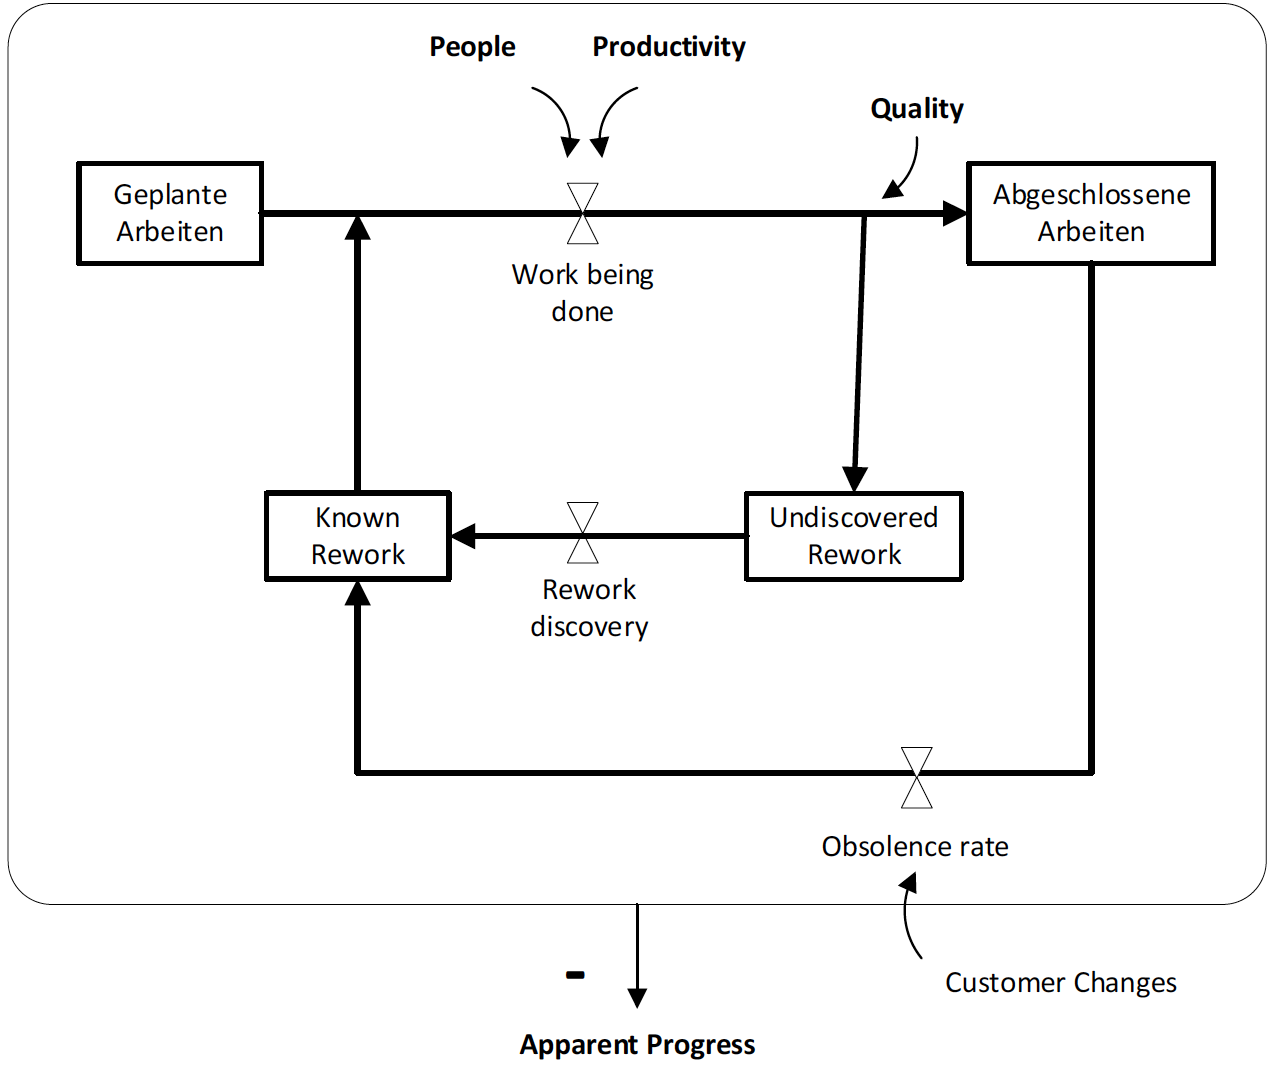
\includegraphics[height=7cm]{img/pm/dynamik_01.png}
			\caption{Projektablauf mit dynamischen Einflüssen}
			\label{fig:pm_dynamik_01}
		\end{figure}
		\noindent
		Korrekt geplante Projekte (ohne Reserven) können nach dieser Logik immer ins Hintertreffen kommen.
		Customer Changes (obsolence rate) reduzieren Fortschritt (apparent progress) massgebend.
		Change Management ist ein Muss!\\
		Korrigieren durch Massnahmen wie bspw. \textbf{Hiring} (weitere Personen ins Projekt), \textbf{Overtime} (Überzeit anordnen), \textbf{Schedule Acceleration} (Arbeitstakt beschleunigen) etc.
		
		\begin{figure}[!htb]
			\centering
			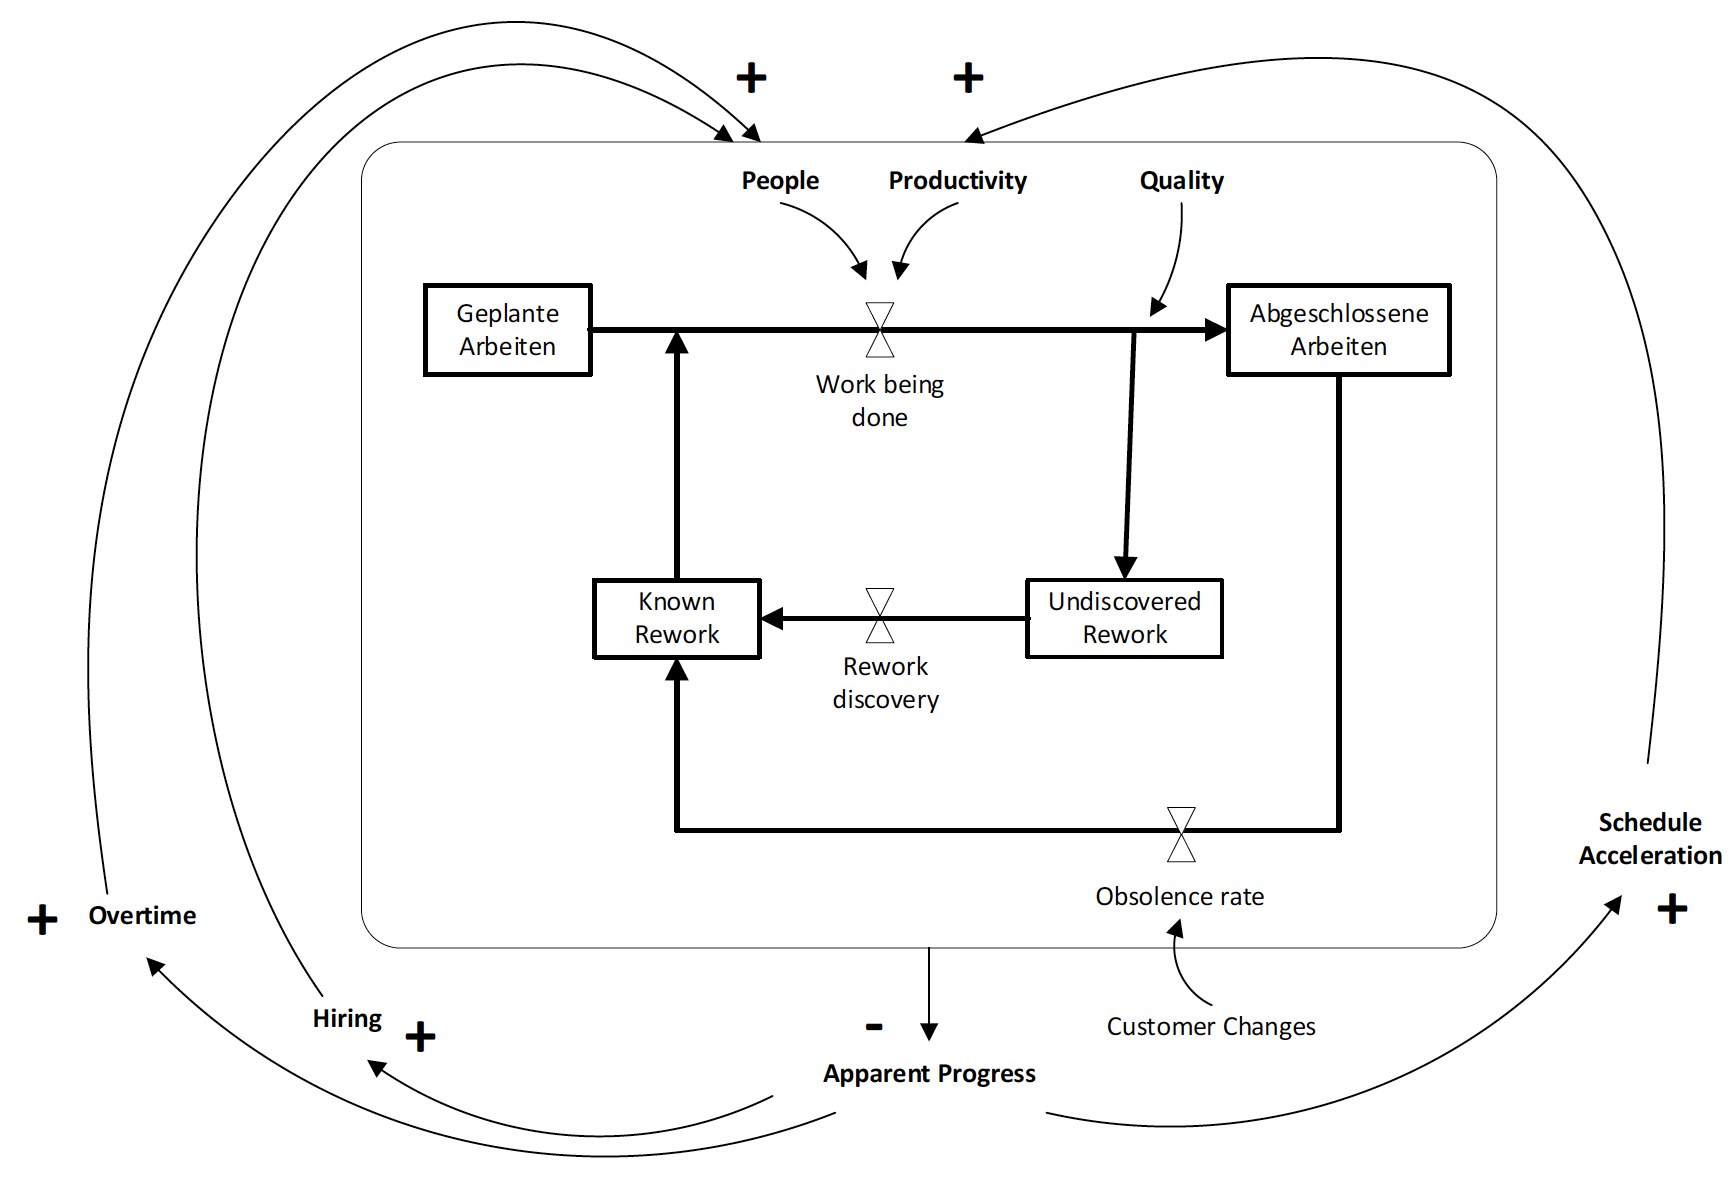
\includegraphics[height=7cm]{img/pm/dynamik_02.png}
			\caption{Projektablauf mit korrigierenden Massnahmen}
			\label{fig:pm_dynamik_02}
		\end{figure}
	
\newpage
		\noindent
	 	Ausgleichende Massnahmen haben jedoch Wechselwirkungen (lösen Reaktionen aus)
	 	\begin{itemize}
	 		\item \textit{Overtime}: mehr Überzeit, desto grösser wird Müdigkeit jedes Projektmitarbeitenden, Burn-Out-Rate steigt, was direkten Einfluss auf Produktivität/Qualität hat, sie sinkt
	 		\item \textit{Hiring}: nominelle Stärkung der Belegschaft, aber durchschnittlicher Ausbildungsstand tiefer, führt zu Qualitätseinbussen
	 		\item \textit{Schedule Acceleration}: Einfluss auf Qualität \& Produktivität, da Koordinationsaufwand grösser wird, Engpässe entstehen, Motivation sinkt
	 	\end{itemize}
 		Es entstehen \textit{self-reinforcing Loops}, welche verstärkend wirken
 		
 		\begin{figure}[!htb]
 			\centering
 			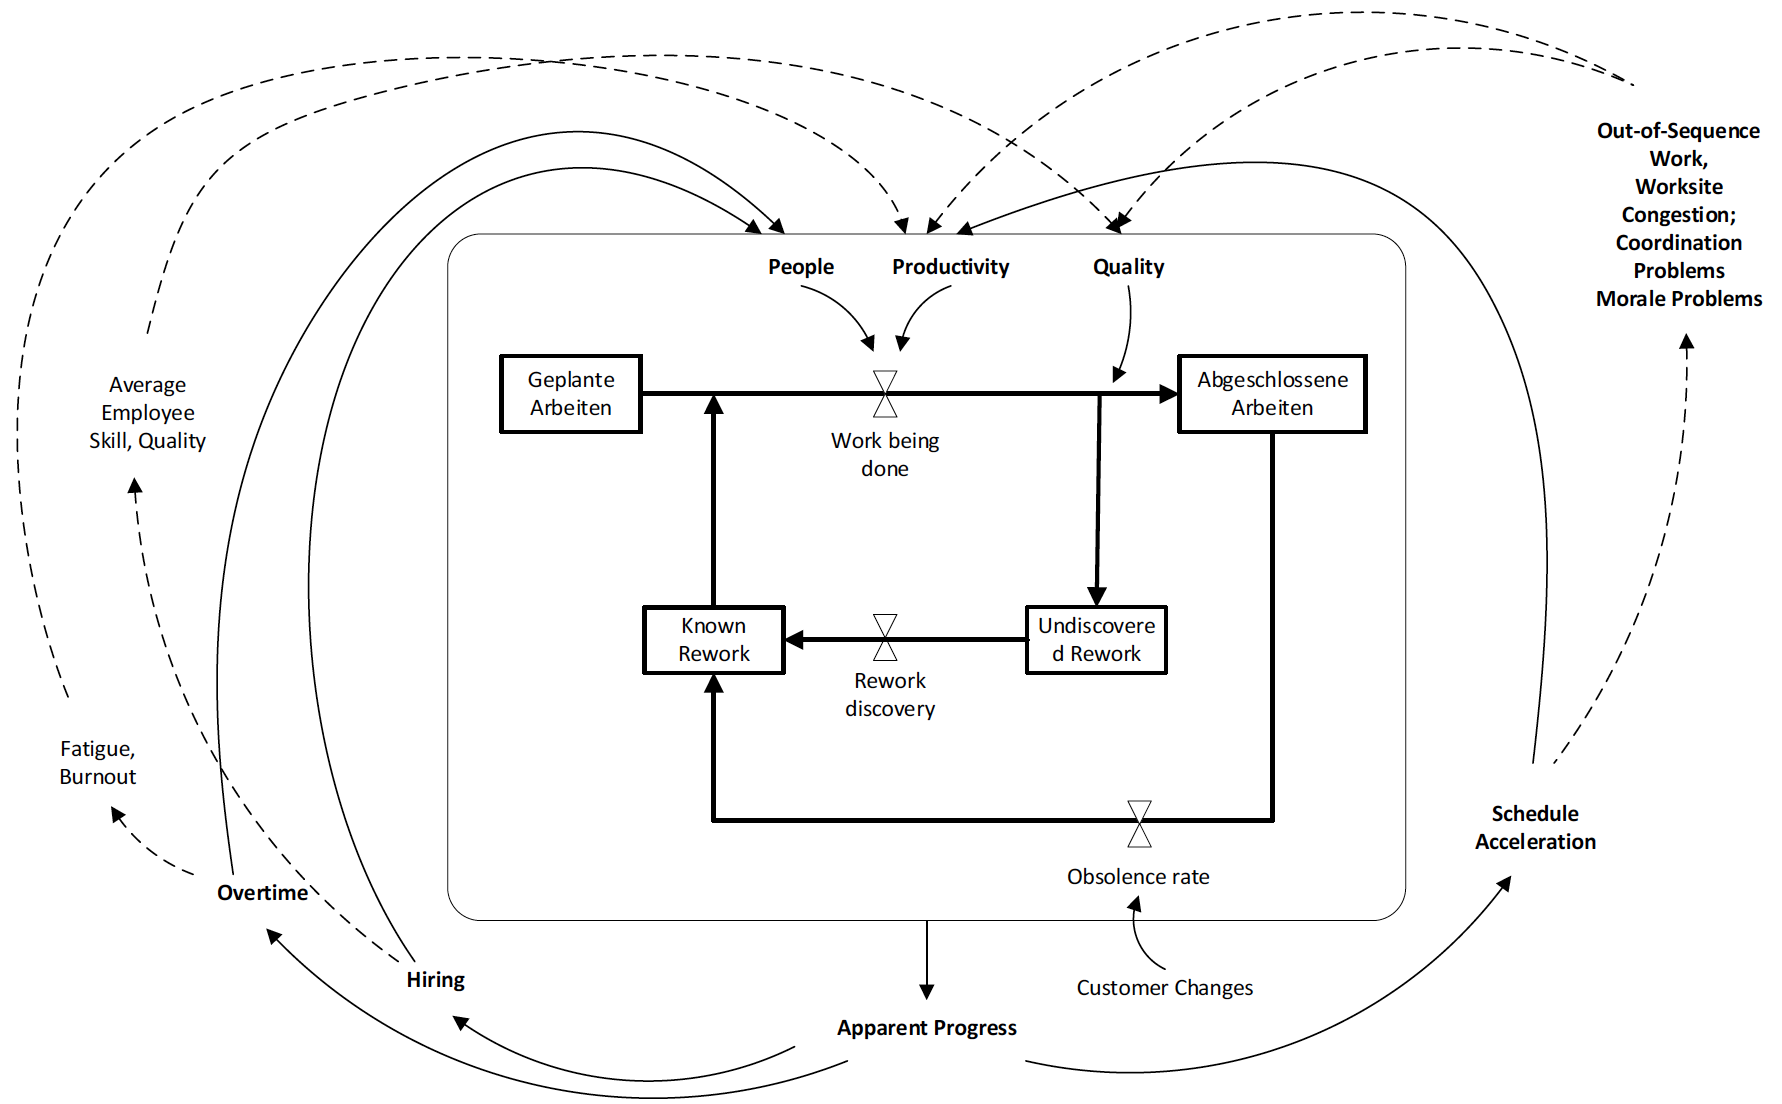
\includegraphics[height=9cm]{img/pm/dynamik_03.png}
 			\caption{Einfluss der Wechselwirkungen auf Projektablauf}
 			\label{fig:pm_dynamik_03}
 		\end{figure}
		\noindent
		Projektleiter muss getroffene Massnahmen sehr kritisch hinterfagen und effektive Wirksamkeit beurteilen.
		Gilt besonders für Personalmassnahmen \textit{("Adding People to a late project makes it even later")}
	
\newpage
				
	\section{Requirement Engineering - Einführung / Setting}
	
		\subsection{Ziel}
		
		\begin{itemize}
			\item Ziel: angestrebter Zustand / erwünschte Wirkung, zukünftige Ergebnisse welche durch bestimmte Massnahmen / Lösungen erreicht werden sollen
			\item Ziele sollen vor Ermittlung der Anforderungen bekannt sein
			\item Ziele beschreiben übergeordnete Erwartungen an Erfolg eines Projekts
			\item Jede einzelne Anforderung muss sich auf ein Ziel zurückführen lassen
			\item Eine Zieldokumentation enthält (aus \textit{Pohl/Rupp S. 67 ff.})
				\begin{itemize}
					\item Ziel-Nummer
					\item Zielname
					\item Zielwert
					\item Messgrösse
					\item Zeitraum
				\end{itemize}
		\end{itemize}
	
		\begin{figure}[!htb]
			\centering
			\begin{subfigure}{.45\textwidth}
				\centering
				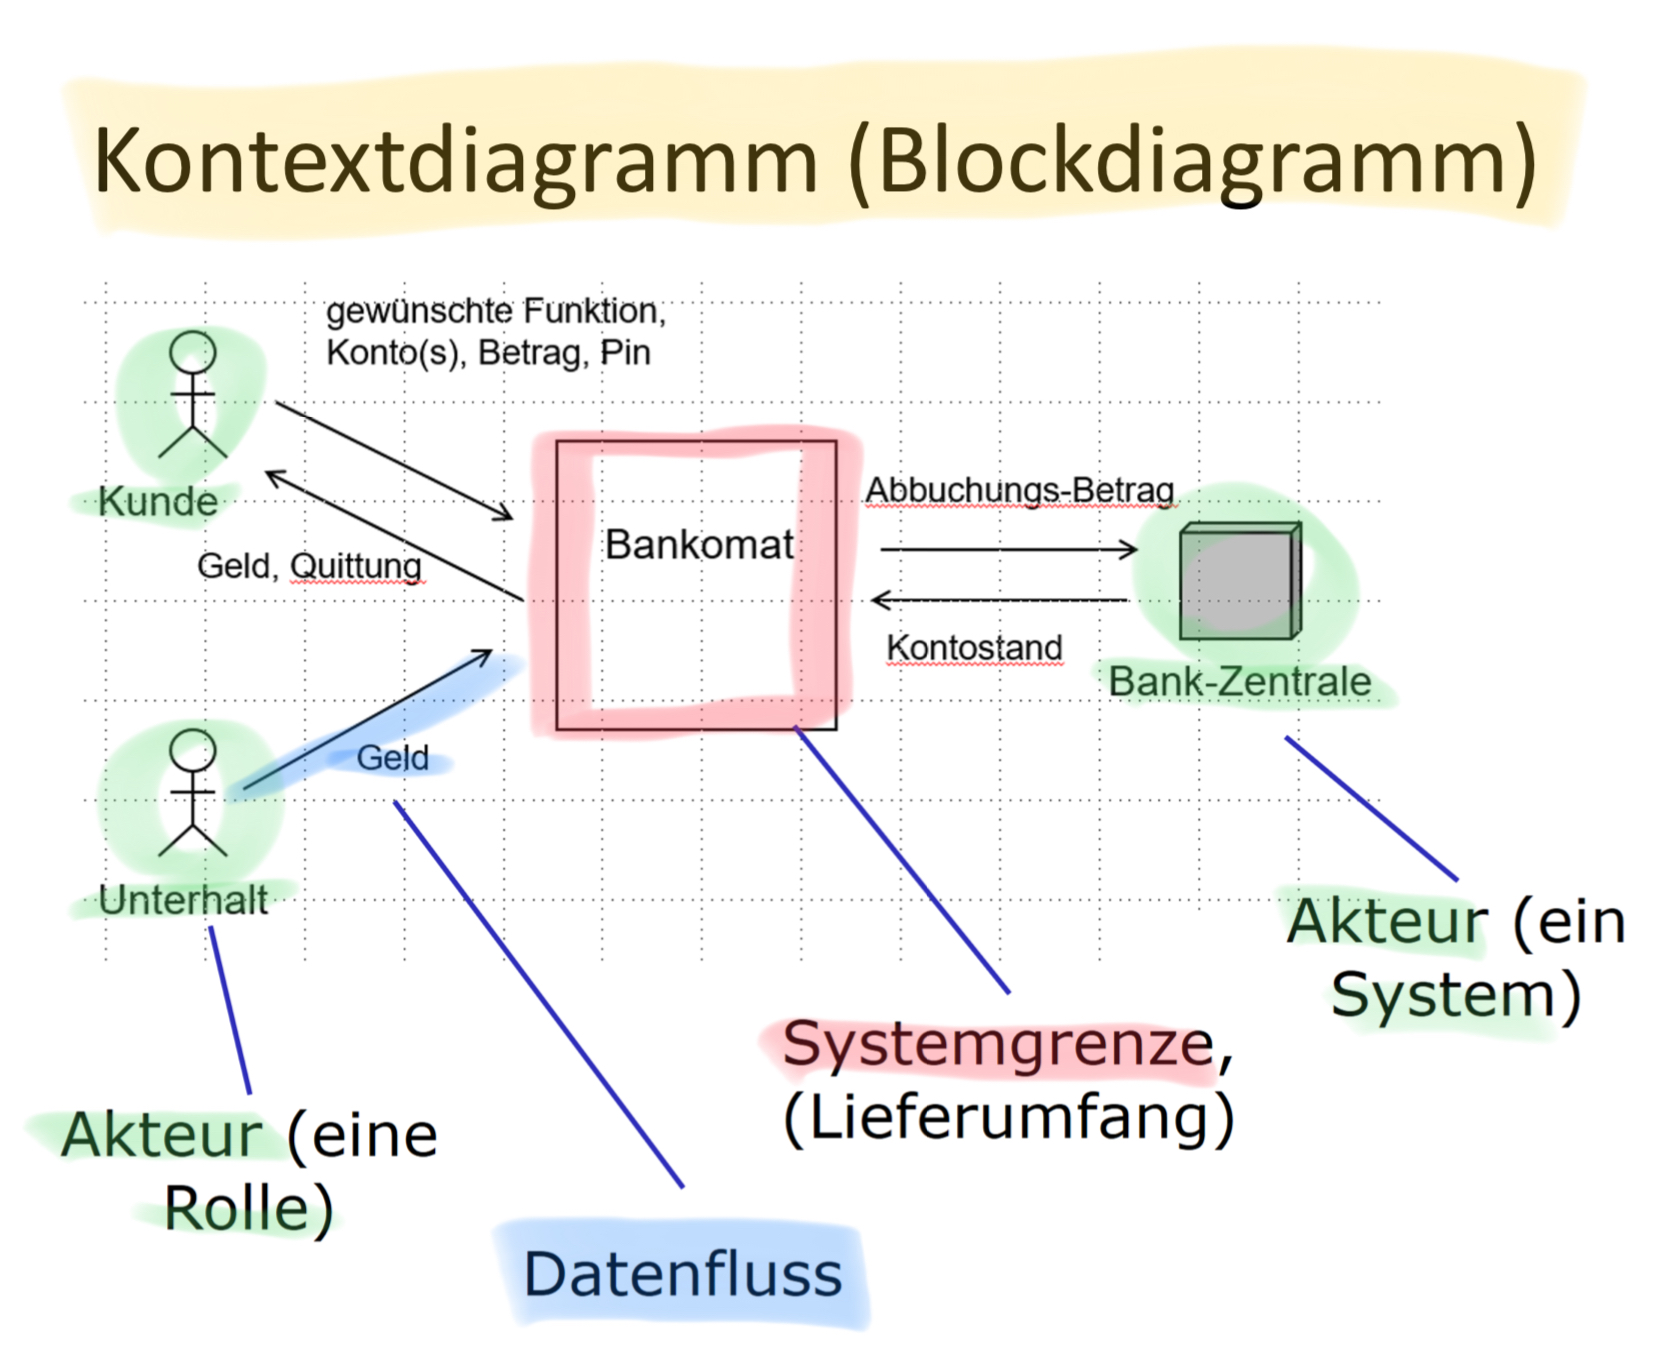
\includegraphics[height=5.5cm]{img/re/01/kontext_block.jpeg}
				\caption{Blockdiagramm (Kontext)}
				\label{fig:re_kontext_block}
			\end{subfigure}
			\begin{subfigure}{.45\textwidth}
				\centering
				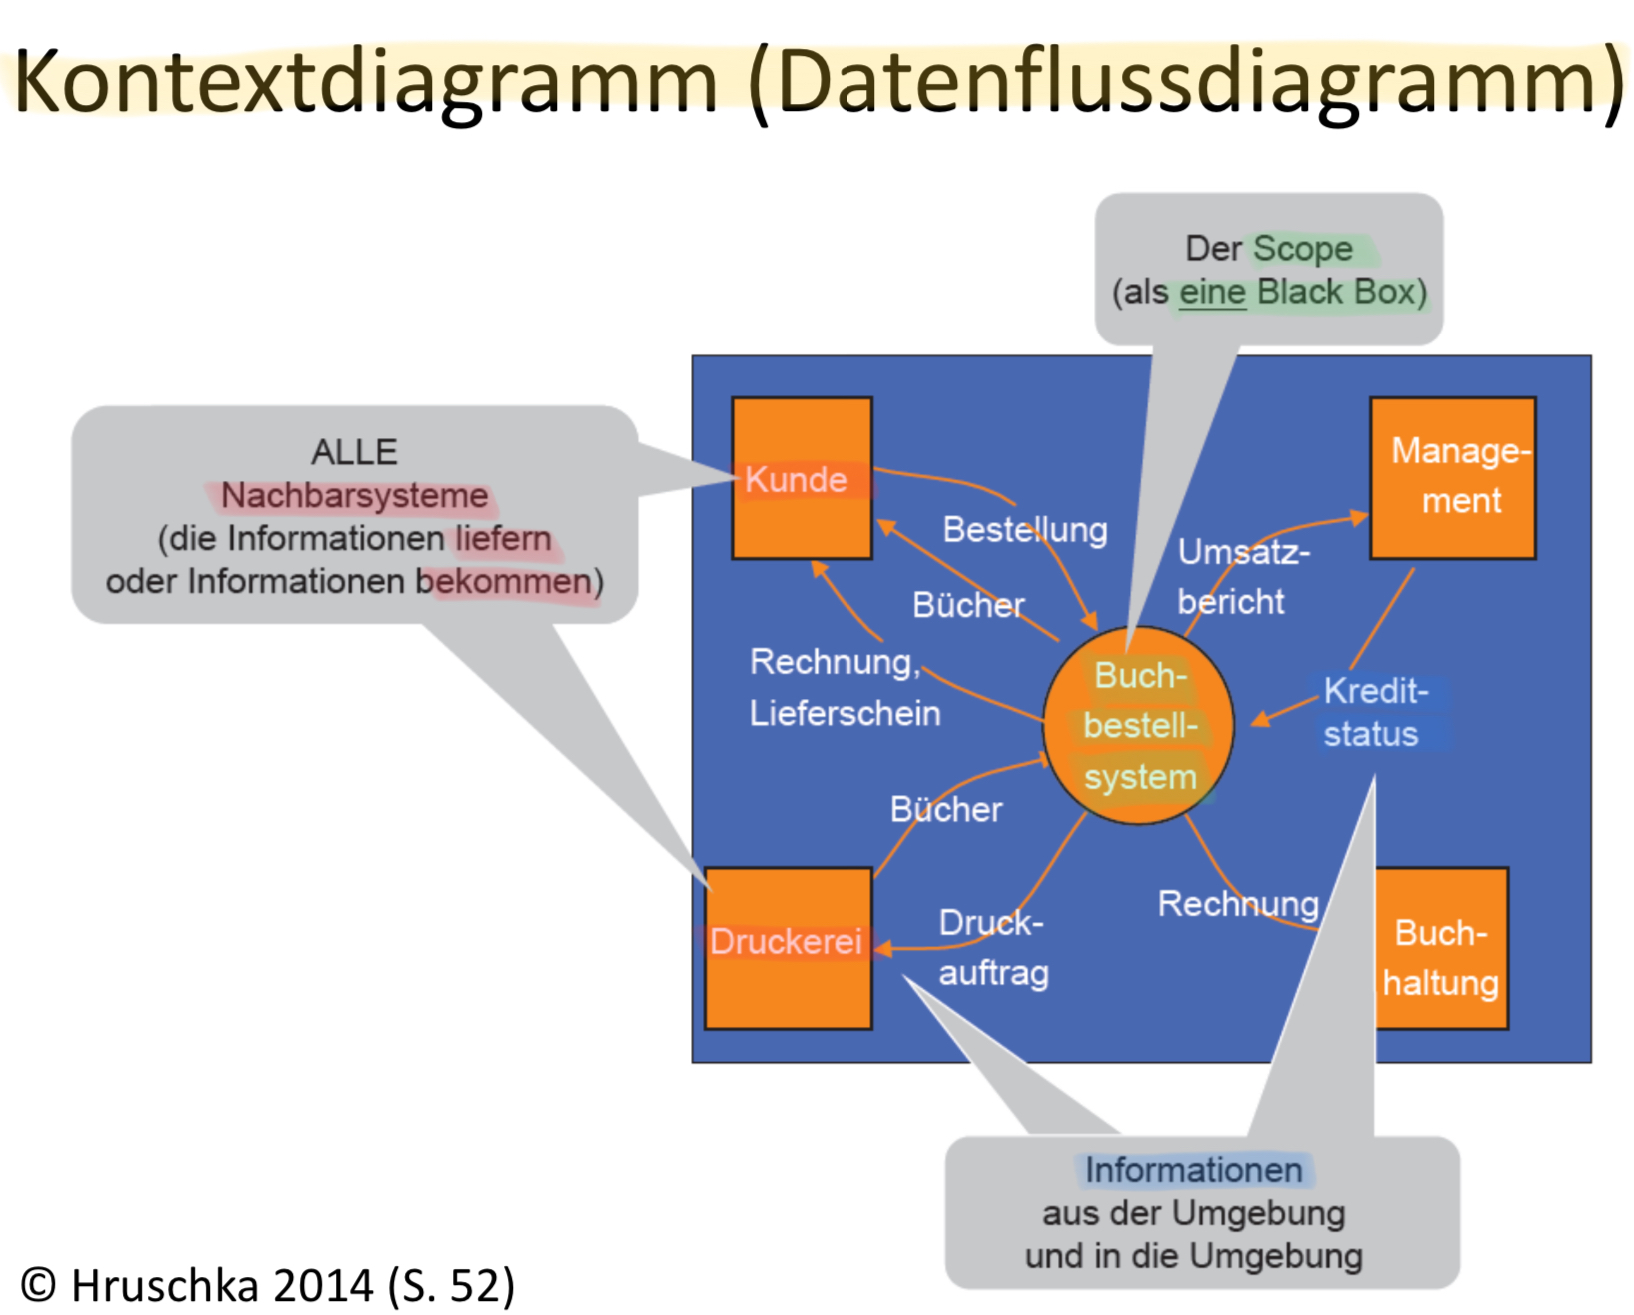
\includegraphics[height=5.5cm]{img/re/01/kontext_datenfluss.jpeg}
				\caption{Datenflussdiagramm (Kontext)}
				\label{fig:re_kontext_datenfluss}
			\end{subfigure}
			\caption{Kontextdiagramme}
			\label{fig:re_kontext_dias}
		\end{figure}
	
			\paragraph{Typische Fehler in einem Kontextdiagramm}
			
			\begin{itemize}
				\item Zusammenhänge ausserhalb, die das System gar nicht betreffen
				\item Unspezifizierte Ein- und Ausgaben im System
				\item Nicht identifizierte Nachbarsysteme
			\end{itemize}
		
		\subsection{Stakeholder}
		
		\begin{itemize}
			\item Werden in einer Stakeholdertabelle festgehalten
			\item Benötigt werden dabei pro Stakeholder mindestens:
				\begin{itemize}
					\item Seine Rolle im System
					\item Name
					\item Wissen
					\item Interessen
				\end{itemize}
		\end{itemize}
		\vspace{1em}
		\noindent
		Es gilt ebenfalls zu klären:
		Was ist die\textbf{Aufgabe} des Stakeholders, wofür ist der Stakeholder \textbf{verantwortlich}, welche \textbf{Weisungsbefugnis} hat der Stahekolder, welche \textbf{Ziele} sollen vom Stakeholder erreicht werden, welche \textbf{Freigaben} kann der Stakeholder zu geben, auf welche Informationen hat der Stakeholder \textbf{Zugriff}, über welche \textbf{Kommunikationswege} werden Informationen ausgetauscht, wann erhält der Stakeholder \textbf{Feedback} zu seinen gelieferten Informationen, welche verantwortlichen \textbf{Personen} werden in welchen \textbf{Situationen} vom Stakeholder informiert, mit wem \textbf{koordiniert} der Stakeholder bestimmte Anforderungen, welche \textbf{Zugriffsrechte} erhält der Stakeholder für das Anforderungsrepository, für welche Fachgebiete ist der Stakeholder offizieller \textbf{Ansprechpartner}?
		
\newpage

		\subsection{RE - Komponenten}
			
		Requirement Engineering setzt sich aus R-Development (Entwicklung) und R-Management (Verwaltung) zusammen.
		Anforderungen können dabei sein: Geschäftprozesse, Geschäftsfälle, Standards, technische Rahmenbedingungen, Funktionalitäten, qualitative Bestimmungen, Geschäftsregeln, Prototypen, Screens etc.\\
		$\rightarrow$ was zur Festlegung der zu entwickelnden Dienstleistung gebraucht wird
		
		\begin{itemize}
			\item Development setzt sich zusammen aus
				\begin{description}
					\item[Elicitation] (Erheben, Ermitteln) welche Erhebungstechniken eignen sich für welche speziellen Informationsbedürfnisse?
					Vorgehen, wenn man etwas in Erfahrung bringen will/soll?
					\item[Analysis] (Analyse, Auswertung) wie Resultate der Erhebung auswerten? (Strukturieren, Zusammenhänge herstellen, Lücken aufdecken etc.)
					\item[Specification] (Spezifikation, Dokumentation) Welche Artefakte, Dokumente, Modelle, Ergebnisse etc. sollen angelegt werden, um das System adäquat zu beschreiben?
					Verständlich und sinnvoll für die Stakeholder?
					\item[Validation] (Validierung) Wie eignet man sich mit entscheidungsrelevanten Stakeholdern auf eine zu realisierende Version? (Prüfen \& Priorisieren der Anforderungen etc.)
				\end{description}
			\item \textbf{Management (Verwaltung)}: Wie / wo werden alle notwendigen Dokumente der Anforderungsentwicklung verwaltet, um einen Überblick zu behalten?
		\end{itemize}
		
	\section{Requirement Engineering - Anforderungen ermitteln}
	
		\subsection{Klassifizieren von Stakeholder-Inputs}
		
		Bedürfnisse (Anforderungsinformationen) müssen verschiedenen Kategorieren zugeordnet werden:
		
		\begin{itemize}
			\item \textbf{Geschäftsanforderungen}\\
			Alles, was finanziellen/geschäftlichen Vorteil auf dem Markt beschreibt, das Kunden oder Unternehmen mit dem Produkt erzielen möchten.
			Kann bspw. mit einem Wert assoziiert werden \textit{(Der Marktanteil wird um X\% erhöht)}
			\item \textbf{Anwendungsfälle und -szenarien}\\
			Allgemeine Aussagen zu Benutzerzielen/Geschäftsausgaben, die die Benutzer ausführen müssen.
			Kann mittels eines Anwendungsszenarios dargestellt/ausgedrückt werden, bspw. \textit{Ich möchte ein Adressetikett für ein versendetes Paket ausdrucken können}
			\item \textbf{Geschäftsregeln}\\
			Wenn nur bestimmte Benutzerklassen unter bestimmten Bedingungen einer Aktivität nachgehen können, bspw. \textit{Chemiker soll nur Chemikale von Gefahrenstufe 1 bestellen können, wenn er für diese Stufe geschult wurde}
			\item \textbf{Funktionelle Anforderungen}\\
			Beschreiben erkennbares Verhalten des Systems unter bestimmten Bedingungen sowie Tätigkeiten, die ein Benutzer mithilfe des Systems verrichten kann, bspw. \textit{Steigt der Druck über 40 bar, muss das entsprechende Warnlich aufleuchten}
			\item \textbf{Qualitätsmerkmale}\\
			Geben Aufschluss darüber, wie gut das System bestimmte Aufgaben ausführt.
			\item \textbf{Anforderungen an die externe Schnittstelle}\\
			Beschreiben die Schnittstelle zwischen einem System und dem Rest der Welt.
			\item \textbf{Einschränkungen}\\
			Einschränkungen in Design \& Implementierung begrenzen verfügbare Optionen des Entwickler.
			\item \textbf{Datendefinitionen}\\
			Beschreiben Vorgabewerte, Datentyp oder Formate, die vom Stakeholder gewünscht/verlangt werden.
			\item \textbf{Lösungsideen}\\
			Konkrete Verfahren oder Anforderungen, welche eine Interaktion mit dem System beschreiben, welches erforderlich ist, um bestimmte Tätigkeiten zu verrichten.
		\end{itemize}
	
\newpage
	
		\subsection{Ermitteln}
		
			\begin{itemize}
				\item Was wissen wir? (bekanntes Wissen)
				\item Was wissen wir noch nicht? (unbekanntes Wissen)
				\item Wie bringen wir "Nichtwissen" in Erfahrung? Welche Anforderungsquellen/Erhebungstechniken?
				\item Wie dokumentieren wir unser Wissen, was soll/muss dokumentiert werden?
				\item Wie überprüfen/validieren wir unser Wissen?
			\end{itemize}
	
		\subsection{7 Product Dimensions}
		
		\begin{figure}[!htb]
			\centering
			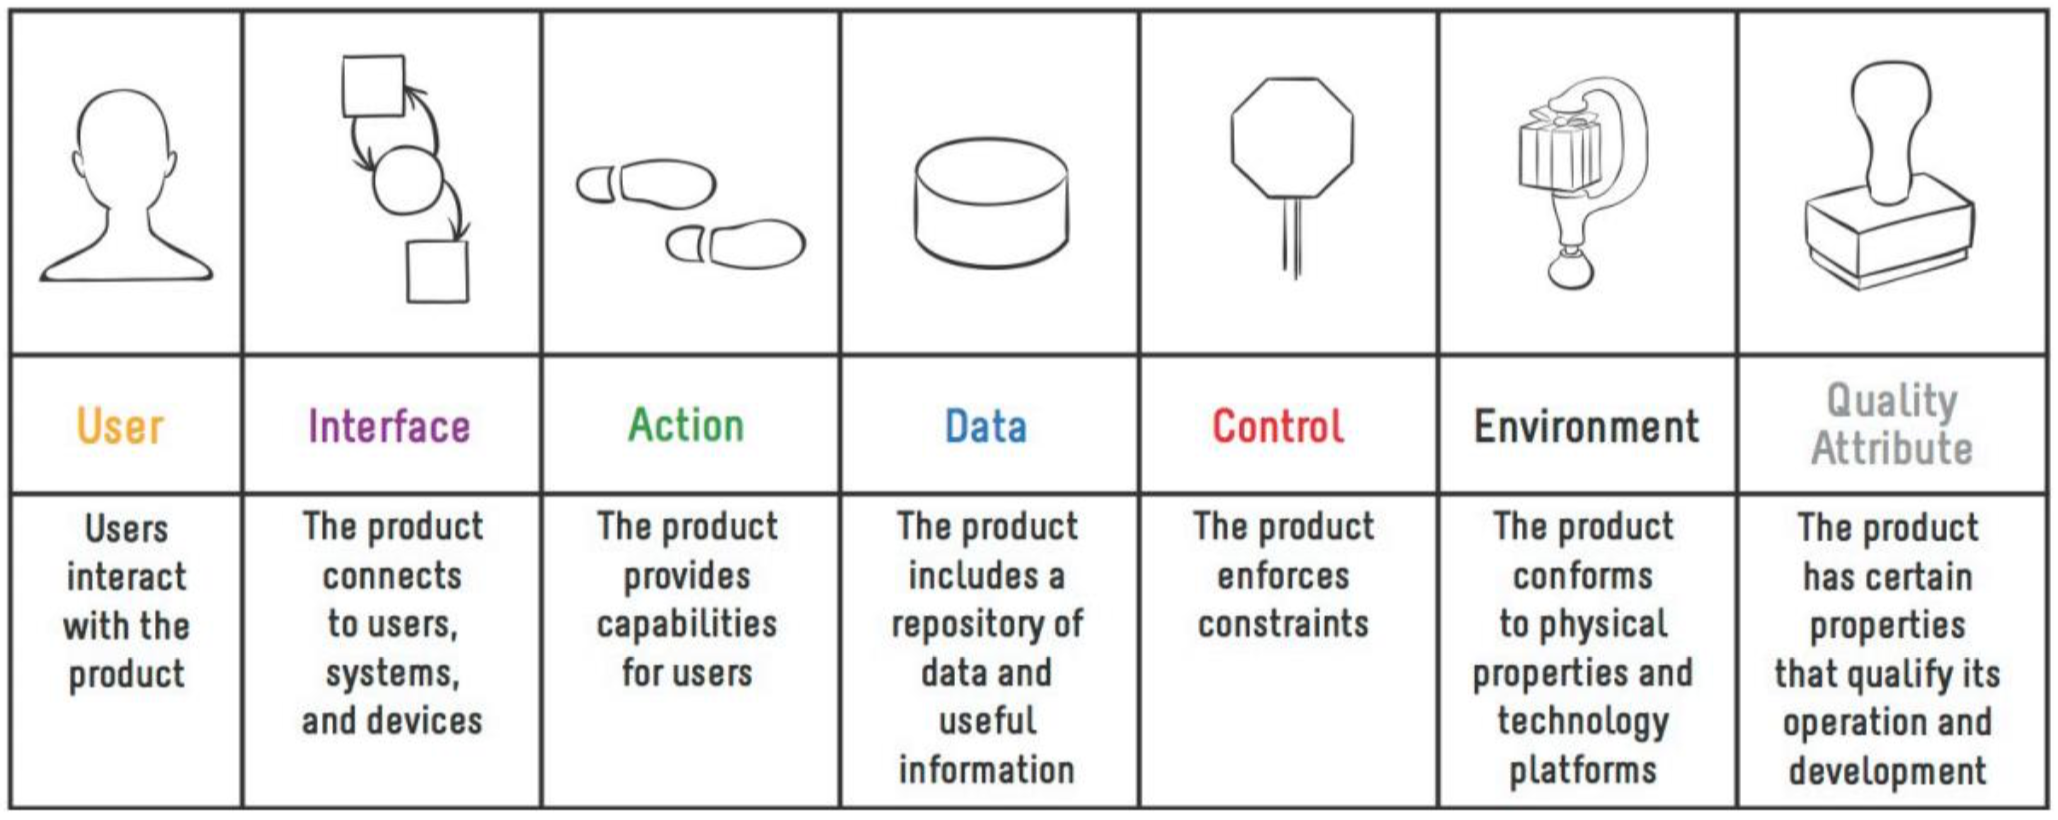
\includegraphics[height=4cm]{img/re/02/product_dimensions.png}
			\caption{Die 7 Produktdimensionen}
			\label{fig:re_product_dimensions}
		\end{figure}
	
		\begin{description}
			\item[User] Wer initiiert eine Aktion und was sind die Ziele? Wer erhält Output des Produkts?
			\item[Interface] Welche Schnittstellen senden Daten/Nachrichten zu oder aus dem Produkt?
			\item[Action] Welche Aktivitäten erfüllen die Bedürfnisse des Nutzers?
			\item[Data] Welche Daten benötigen die Nutzer vom Produkt?
			\item[Control] Welches sind die Policies, Regulationen und Geschäftsregeln, \\
				die das Produkt erzwingen muss?
			\item[Environment] Wo wird das Produkt genutzt? Welche Software/Hardware wird genutzt, \\
				um das Produkt zu entwickeln/bedienen?
			\item[Quality Attribute] Welches sind die Service-Stufen für Availability, Installability, Usability etc.?
		\end{description}
	
		\subsection{W-Fragen für bspw. Interviews}
		
		\begin{figure}[!htb]
			\centering
			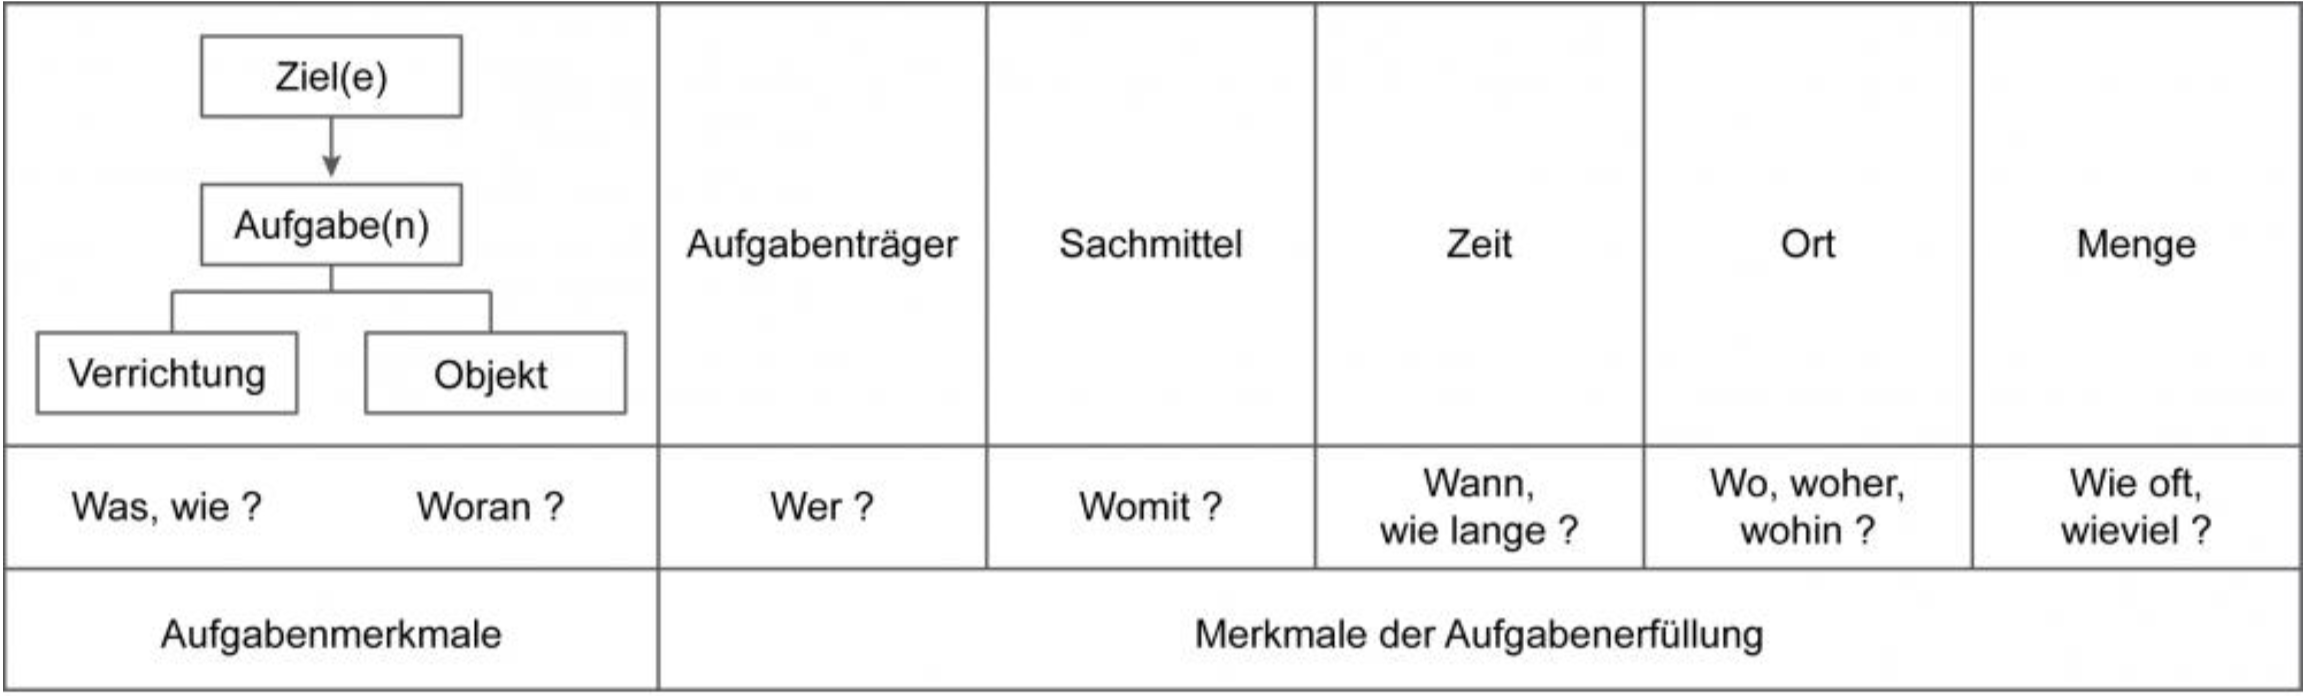
\includegraphics[height=3.5cm]{img/re/02/w_fragen.png}
			\caption{Einteilung der W-Fragen}
			\label{fig:re_w_fragen}
		\end{figure}
	
			\paragraph{K.R.O.K.U.S. Regel zur Formulierung von Fragen}
			
			\begin{description}
				\item[K] Kurze Fragen stellen
				\item[R] Redundante fragen vermeiden
				\item[O] Offene Fragen stellen
				\item[K] Konkrete Fragen stellen
				\item[U] Unterfragen (\& Kettenfragen) vermeiden
				\item[S] Suggestive Fragen vermeiden
			\end{description}
	
\newpage

	\section{Requirement Engineering - Anforderungen dokumentieren}
	
	
	
	
	
	
	
	
	
\end{document}
